% Copyright 2009 by Tomasz Mazur
%
% This file may be distributed and/or modified in all ways.


\documentclass[xcolor=pdftex,t,11pt]{beamer}

%%%%%%%%%%%%%%%%%%%%%%%%%%%%%%%%%%
%       SET OPTIONS BELOW        %
%%%%%%%%%%%%%%%%%%%%%%%%%%%%%%%%%%

\usepackage{xspace}
\usepackage{subfig}
\usepackage{adjustbox}
\usepackage{pifont,color,soul}
\usepackage[most]{tcolorbox}
\usepackage{listings}
\usepackage{blindtext}
\usepackage{fancyvrb}
 \usepackage{adjustbox}
\usepackage{xcolor,colortbl}
\usepackage{algorithm,algorithmic}
\usepackage{caption}
\newcommand{\xmark}{\ding{55}}
\definecolor{azure}{rgb}{0.0, 0.5, 1.0}

\lstnewenvironment{queryl}[1][] 
   {\lstset{linewidth=8cm, #1}}
   {}

\usetheme[
% Toggle showing page counter
pagecounter=true,
%
% String to be used between the current page and the
% total page count, e.g. of, /, from, etc.
pageofpages=of,
%
% Defines the shape of bullet points. Available options: circle, square
bullet=circle,
%
% Show a line below the frame title. 
titleline=true,
%
% Set the style of the title page (true for fancy, false for standard)
alternativetitlepage=true,
%
% Institution logo for fancy title page.
% Comment out to remove the logo from the title page.
% IMPORTANT: THERE IS A BUG IN SOME VERSIONS OF PDFLATEX AND FONTS
% ON THE LOGOS ARE NOT RENDERED PROPERLY. IN SUCH A CASE ADD `2` 
% TO THE NAME OF THE LOGO, E.G. comlab2 INSTEAD OF comlab
%titlepagelogo=images/titlepage/ou,
%
% Department footer logo for fancy title page
% Comment out to remove the logo from the footer of the title page/
% IMPORTANT: THERE IS A BUG IN SOME VERSIONS OF PDFLATEX AND FONTS
% ON THE LOGOS ARE NOT RENDERED PROPERLY. IN SUCH A CASE ADD `2` 
% TO THE NAME OF THE LOGO, E.G. comlab2 INSTEAD OF comlab
%titlepagefooterlogo=images/titlepage/comlab,
%
% Institution/department logo for ordinary slides
% Comment this line out to remove the logo from all the pages.
% Available logos are: ou, comlab, comlabinline, comlabou
% IMPORTANT: THERE IS A BUG IN SOME VERSIONS OF PDFLATEX AND FONTS
% ON THE LOGOS ARE NOT RENDERED PROPERLY. IN SUCH A CASE ADD `2` 
% TO THE NAME OF THE LOGO, E.G. comlab2 INSTEAD OF comlab
%ordinarypageslogo=TU-Signet,
%
%
% Add watermark in the bottom right corner
%watermark=<filename>,
%
% Set the height of the watermark.
%watermarkheight=100pt,
%
% The watermark image is 4 times bigger than watermarkheight.
%watermarkheightmult=4,
]{Torino}

% Select color theme. Available options are:
% mininmal, greenandblue, blue, red
\usecolortheme{blue}

%Select different font themes.Available options are:
% default, serif, structurebold, structureitalicserif, structuresmallcapsserif
\usefonttheme{structurebold}


\pgfdeclareimage[height=6ex]{ou-logo}{ou}

\logo{\pgfuseimage{ou-logo}}

\usepackage{pgf}

\pgfdeclareimage[height=6ex]{ou-logo}{ou}

\logo{\pgfuseimage{ou-logo}}

\usepackage{listings}

%% \lstset{language=C,
%%   basicstyle=\normalsize,
%%   linewidth=8cm
%%  }

\usepackage{ifthen}

\usepackage{pgf}
\usepackage{tikz}
\usetikzlibrary{arrows, automata, shapes.multipart, chains, positioning, fit, graphs, spy, shapes, backgrounds, patterns}

\usepackage{color}
\definecolor{light-gray}{gray}{0.80}
\definecolor{green}{rgb}{0.30588, 0.60392, 0.023529}     % #4e9a06


\newenvironment<>{codeblock}[1][]{%
  \setbeamercolor{block title example}{fg=white,bg=blue!75!black}%
  \begin{block}#2[#1]}{\end{block}}

  \newenvironment<>{examplesecond}[1]{%
  \setbeamercolor{block title}{fg=white,bg=blue!75!black}%
  \begin{block}#2{#1}}{\end{block}}

  

%%%%%%%%%%%%%%%%%%%%%%%%%%%%%%%%%%
%       PRESENTATION INFO        %
%%%%%%%%%%%%%%%%%%%%%%%%%%%%%%%%%%

  \title{\fontsize{11}{12}\selectfont Automated Formal Synthesis of Digital Controllers
    \newline
    for State-Space Physical Plants}
\subtitle{CAV 2017}
\institute{\normalsize Diffblue Ltd., \\University ~of ~Oxford, \\Federal University of Amazonas}
\date{}
\author{\normalsize Alessandro Abate, Iury Bessa, Dario Cattaruzza,\\
  Lucas Cordeiro, {\bf Cristina David}, Pascal Kesseli,\\
  Daniel Kroening and Elizabeth Polgreen}

\begin{document}


%%%%%%%%%%%%%%%%%%%%%%%%%%%%%%%%%%
%       SLIDE DEFINITIONS        %
%%%%%%%%%%%%%%%%%%%%%%%%%%%%%%%%%%

\begin{frame}[plain]
  \titlepage
  \vspace{-3.5cm}
    
\includegraphics[width=.15\textwidth]{figures/aec-badge-cav.pdf}
\end{frame}


\begin{frame}{Motivation}

\centering
 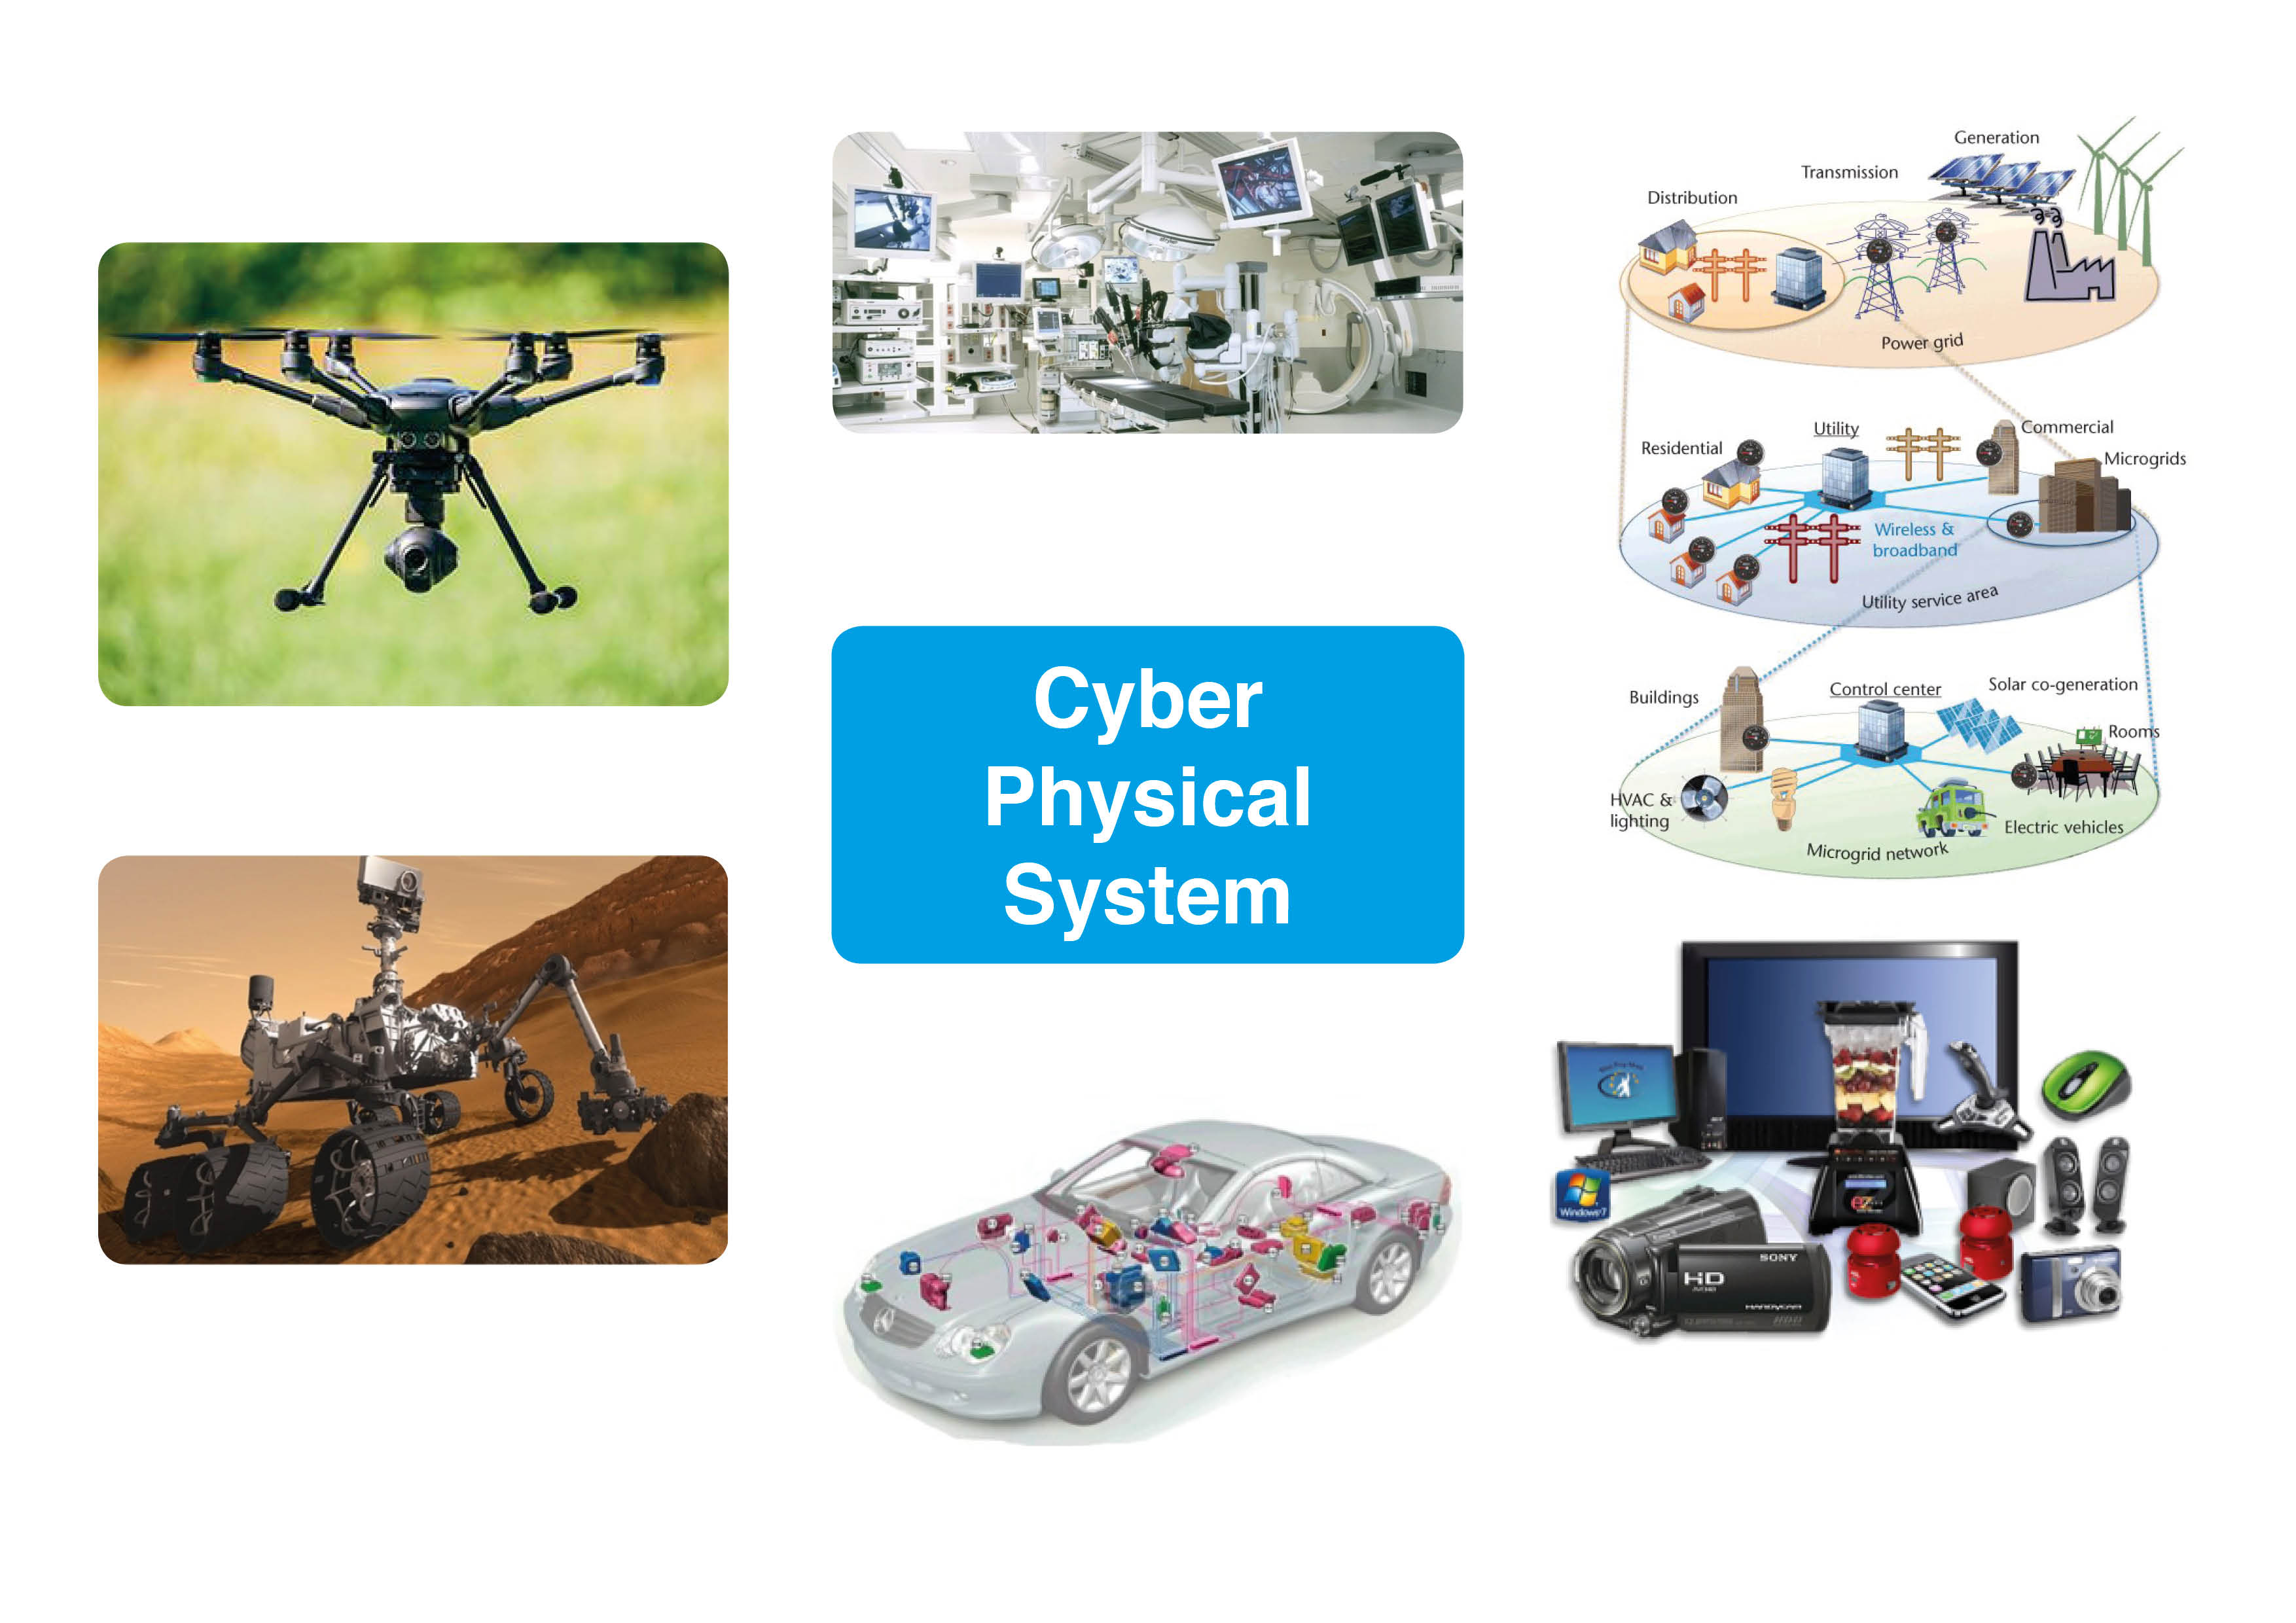
\includegraphics[width=.75\textwidth]{figures/CPS.jpg} 

 
\uncover<2>{
 \vspace{-.5cm}
  \small
{\bf Automatically synthesise feedback digital controllers that ensure
{\color {red} stability} and {\color {red} safety}}}

\end{frame}


\begin{frame}{State-feedback architecture}
\vspace{-1cm}
\begin{center}
  \begin{overprint}
    \onslide<1,2>
    \centerline{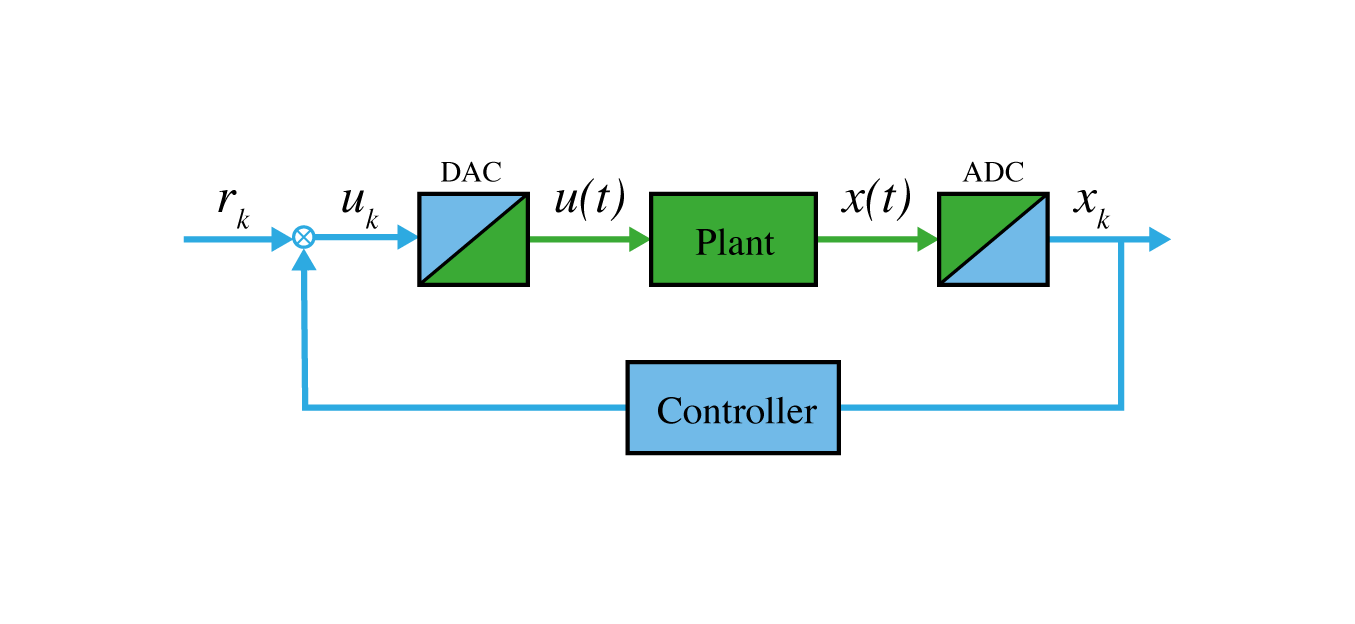
\includegraphics[width=.9\textwidth]{figures/spirals/diagram-15.png}}
    \onslide<3->
    \centerline{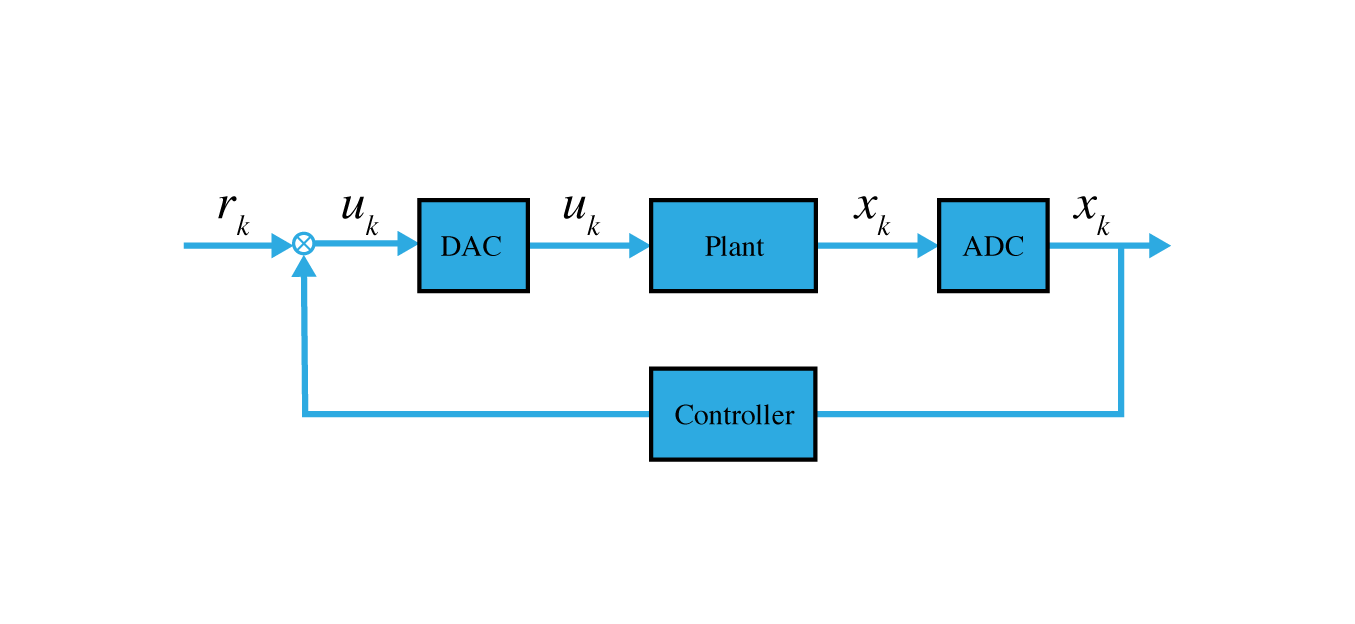
\includegraphics[width=.9\textwidth]{figures/spirals/diagram-16.png}}
  \end{overprint}
  \end{center}
  \vspace{-1cm}
  \only<1,2>{{\bf Continuous-discrete system}}
  \only<3->{{\bf Digital domain}}  
  \begin{itemize}
  \item \only<1,2>{\colorbox{green!70}{Plant:
    \textsc{$\dot{x}(t) = Ax(t)+ Bu(t), \quad t \in \mathbb R_0^+,~x(0)=initial~state$}}}
    \only<3->{\colorbox{azure!70}{Plant:
    \textsc{$x_{k+1} = A x_k+ B u_k, \quad k \in \mathbb \mathbb N,~x_0=initial~state$}}}
  \item \colorbox{azure!70}{State-feedback controller:   \only<1>{$u_k = r_{k} - C x_k$}\only<2->{$u_k = - C x_k$}}
  \item \uncover<4->{Finite precision}  
\end{itemize}
\end{frame}

\begin{frame}{Numerical errors}
\vspace{-1cm}
  \begin{center}
    \only<1>{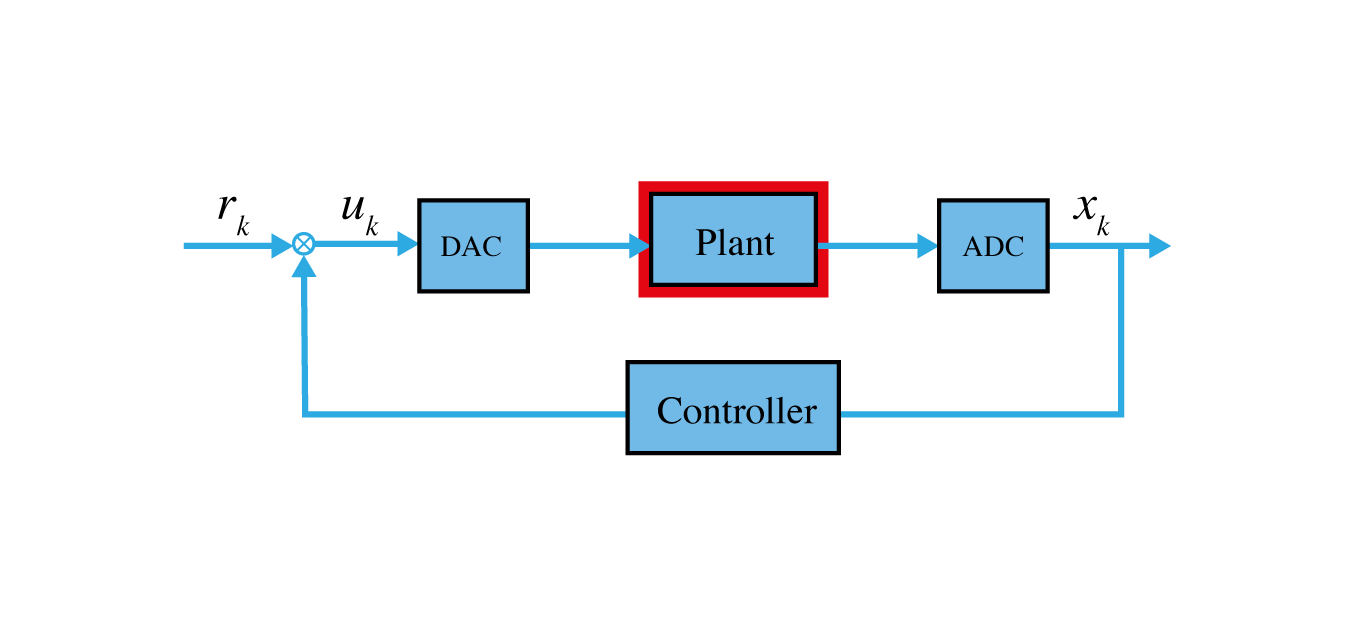
\includegraphics[width=.9\textwidth]{figures/spirals/diagram-18.png}}
    \only<2>{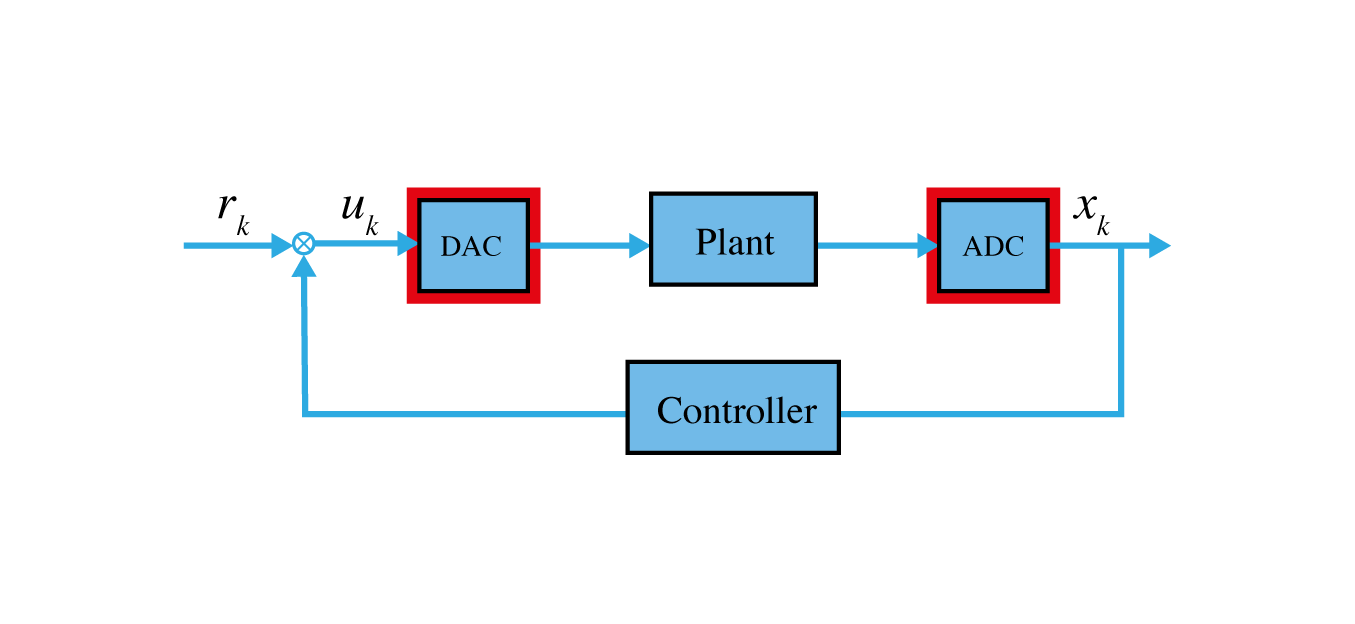
\includegraphics[width=.9\textwidth]{figures/spirals/diagram-19.png}}
    \only<3->{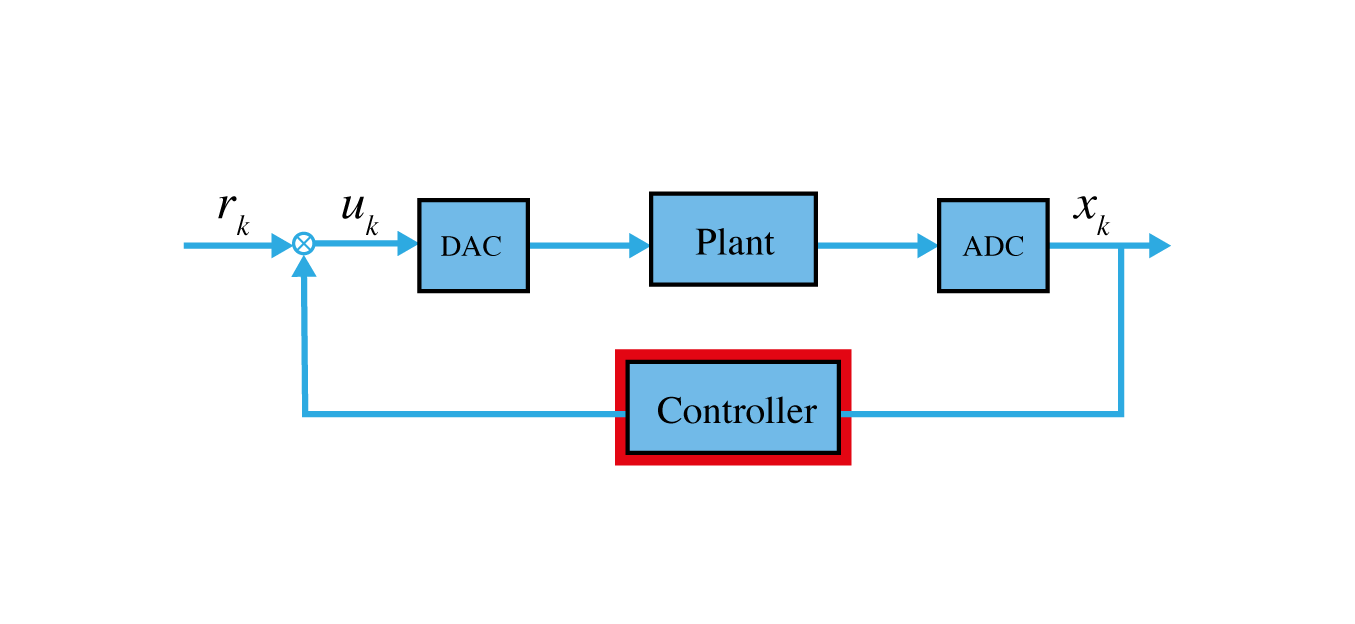
\includegraphics[width=.9\textwidth]{figures/spirals/diagram-20.png}}
  \end{center}
  \vspace{-1cm}
  \begin{itemize}
  \item \uncover<1->{{\bf Truncation and rounding on the plant (interval arithmetic)}}
  \item  \uncover<2->{{\bf Truncation on the converters (additive noise)}}
  \item \uncover<3->{{\bf Rounding on the controller (additive noise)}}
  \end{itemize}  
 
\end{frame}  

\begin{frame}{Our approach}
  \vspace{-.5cm}
  \centerline{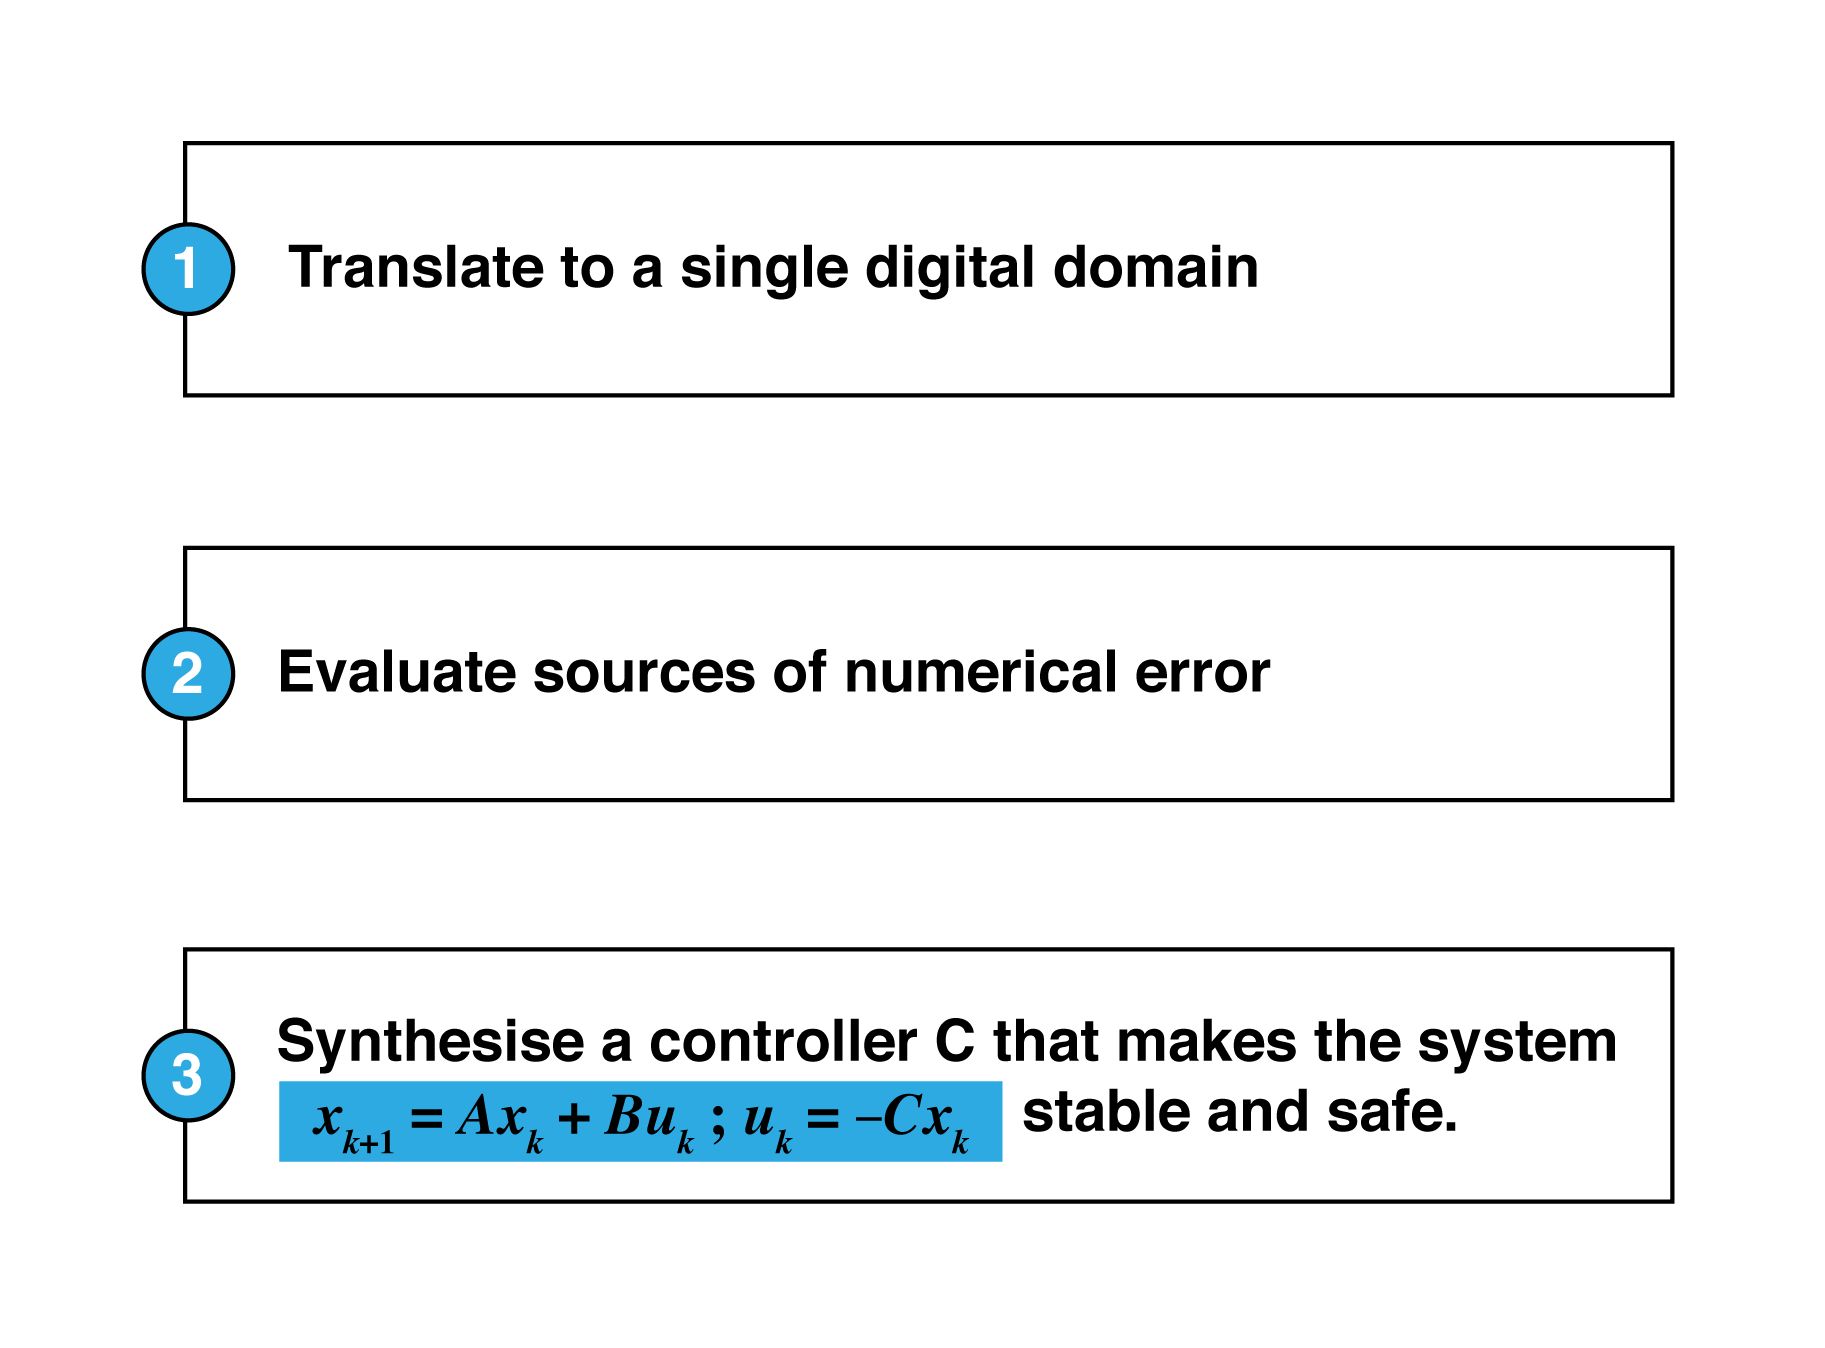
\includegraphics[width=.9\textwidth]{figures/spirals/diagram-28.png}}
\end{frame}
  

\begin{frame}{Stability \only<5>{and safety}}

  \small

  {\bf A system \colorbox{azure!70}{
    \textsc{$x_{k+1} = A x_k+ B u_k, u_k = - C x_k$}} is
  asymptotically stable if its executions converge to an equilibrium point,
  when starting from any states in a neighborhood of
the point.}

\begin{center}
\begin{overprint}
  \onslide<2>
  \centerline{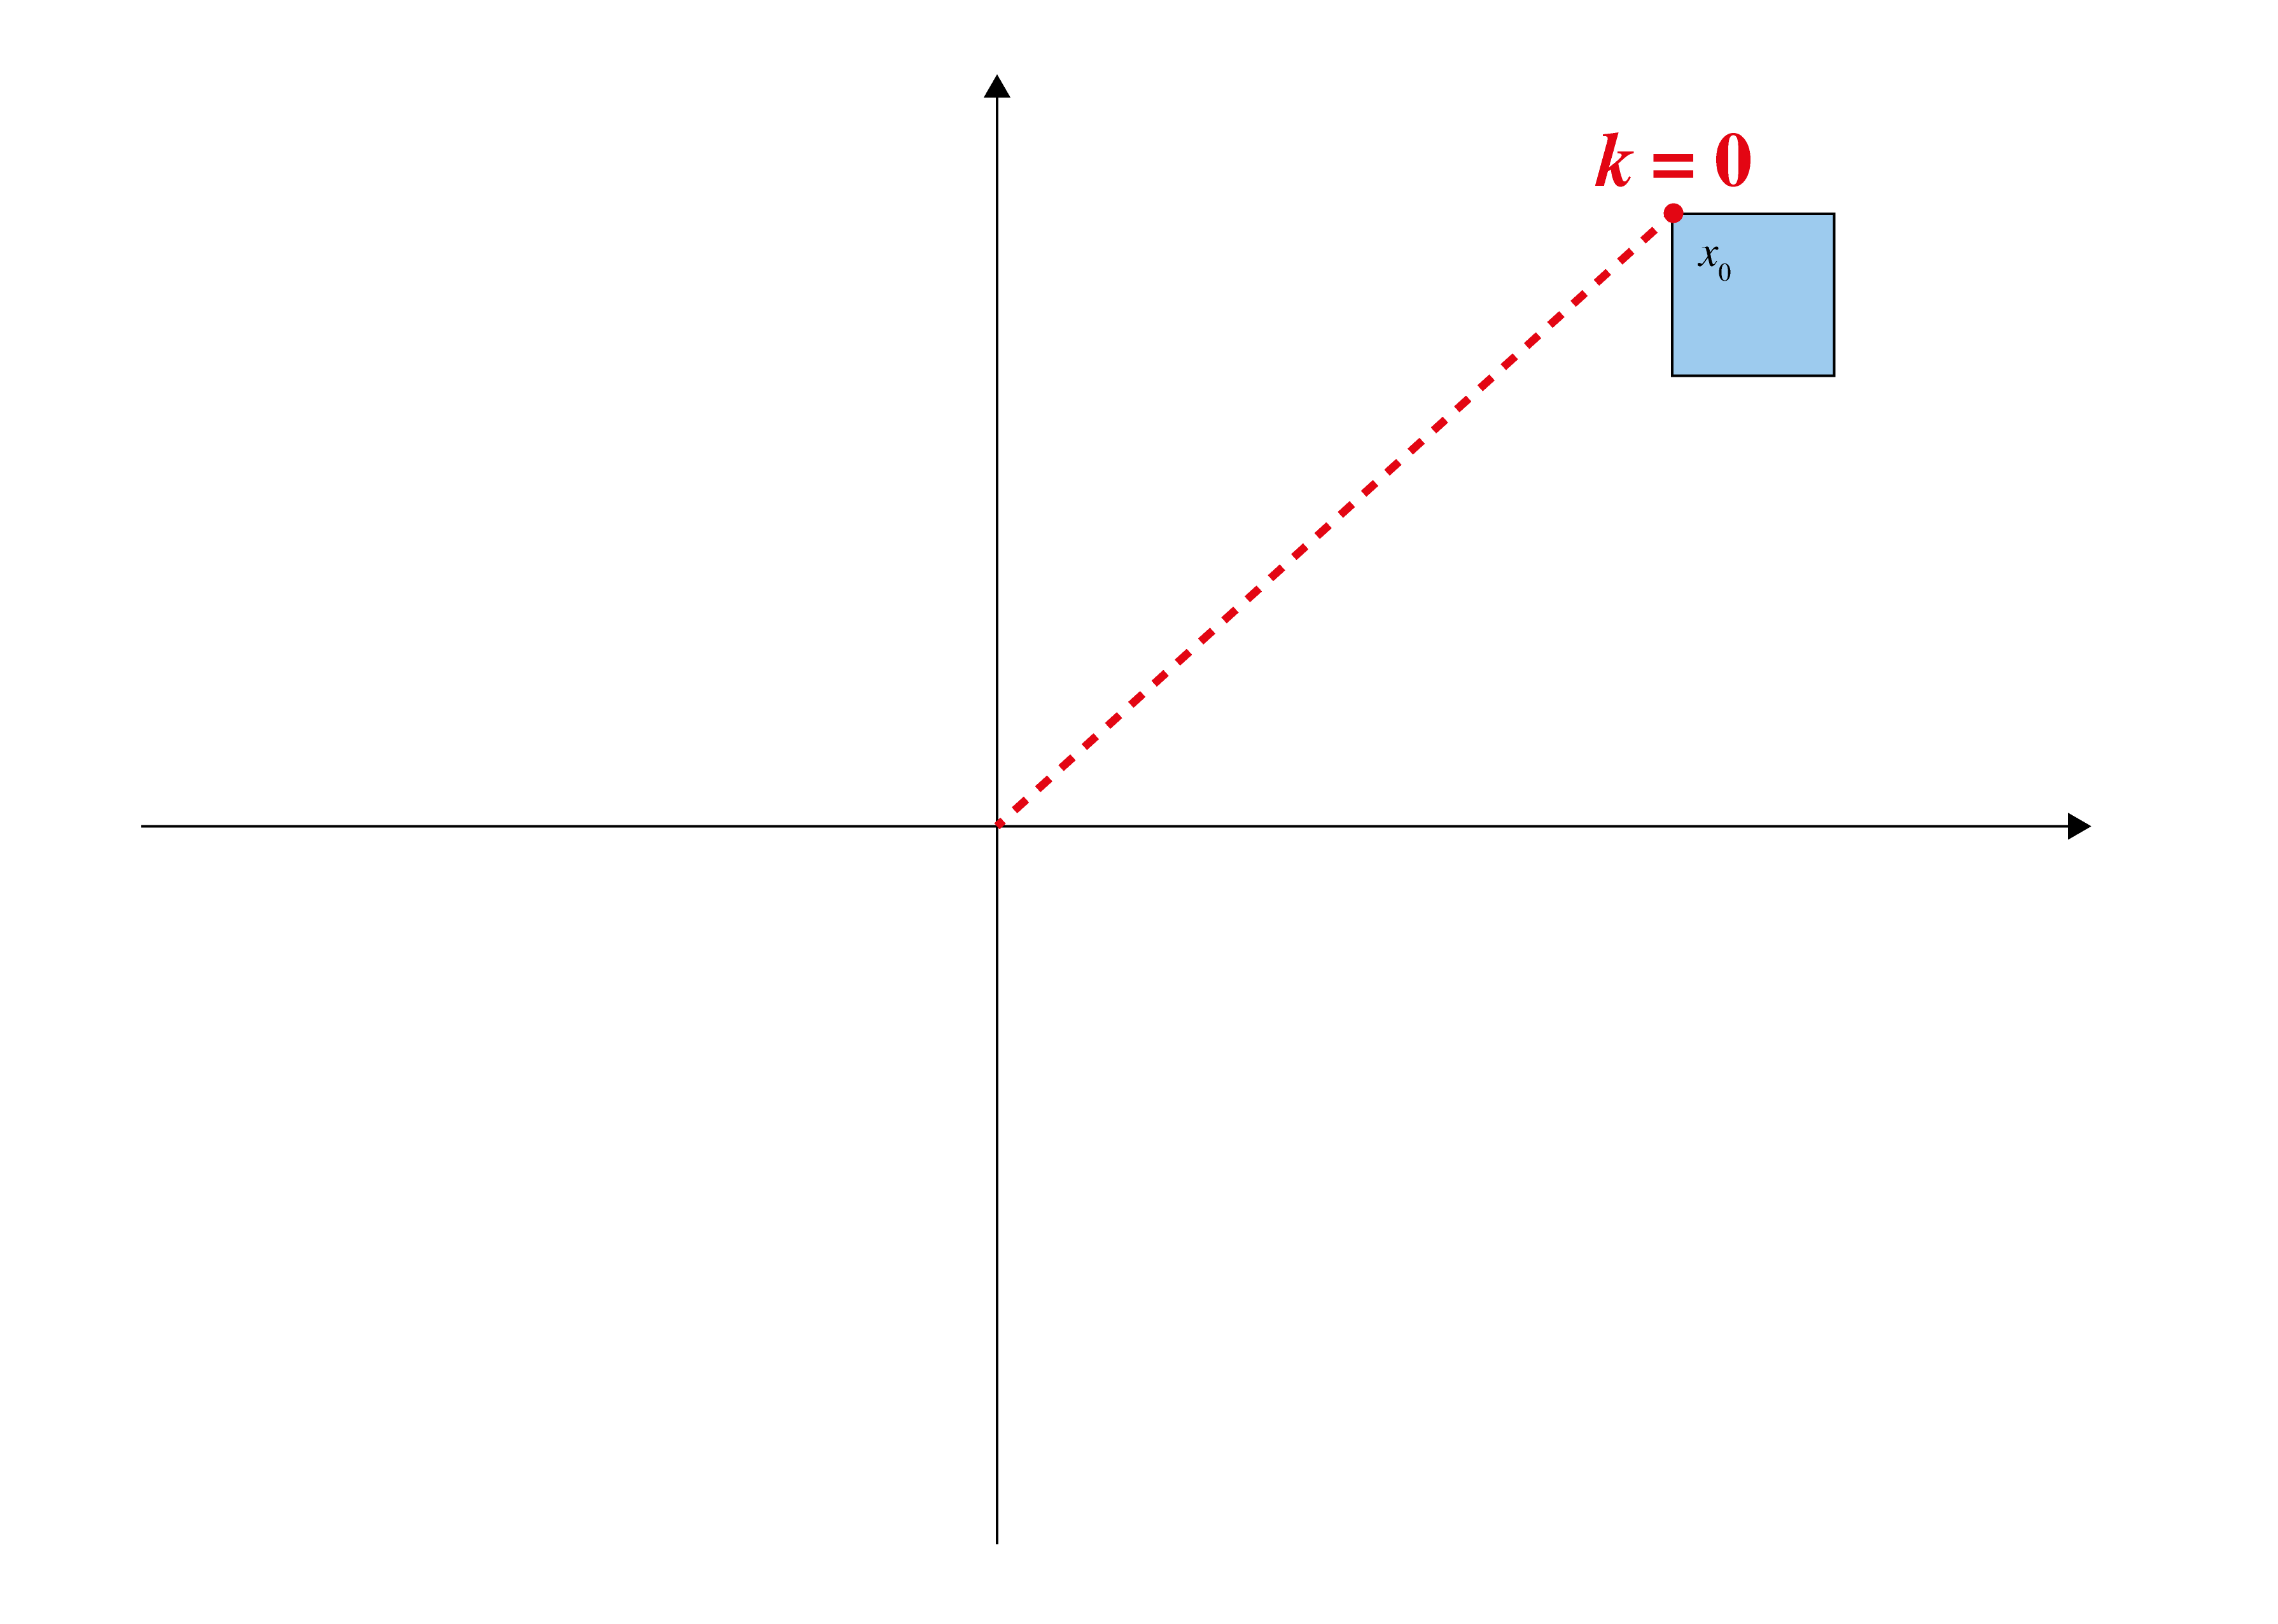
\includegraphics[width=.65\textwidth]{figures/spirals/Spirals-21.png}}
  \onslide<3>
  \centerline{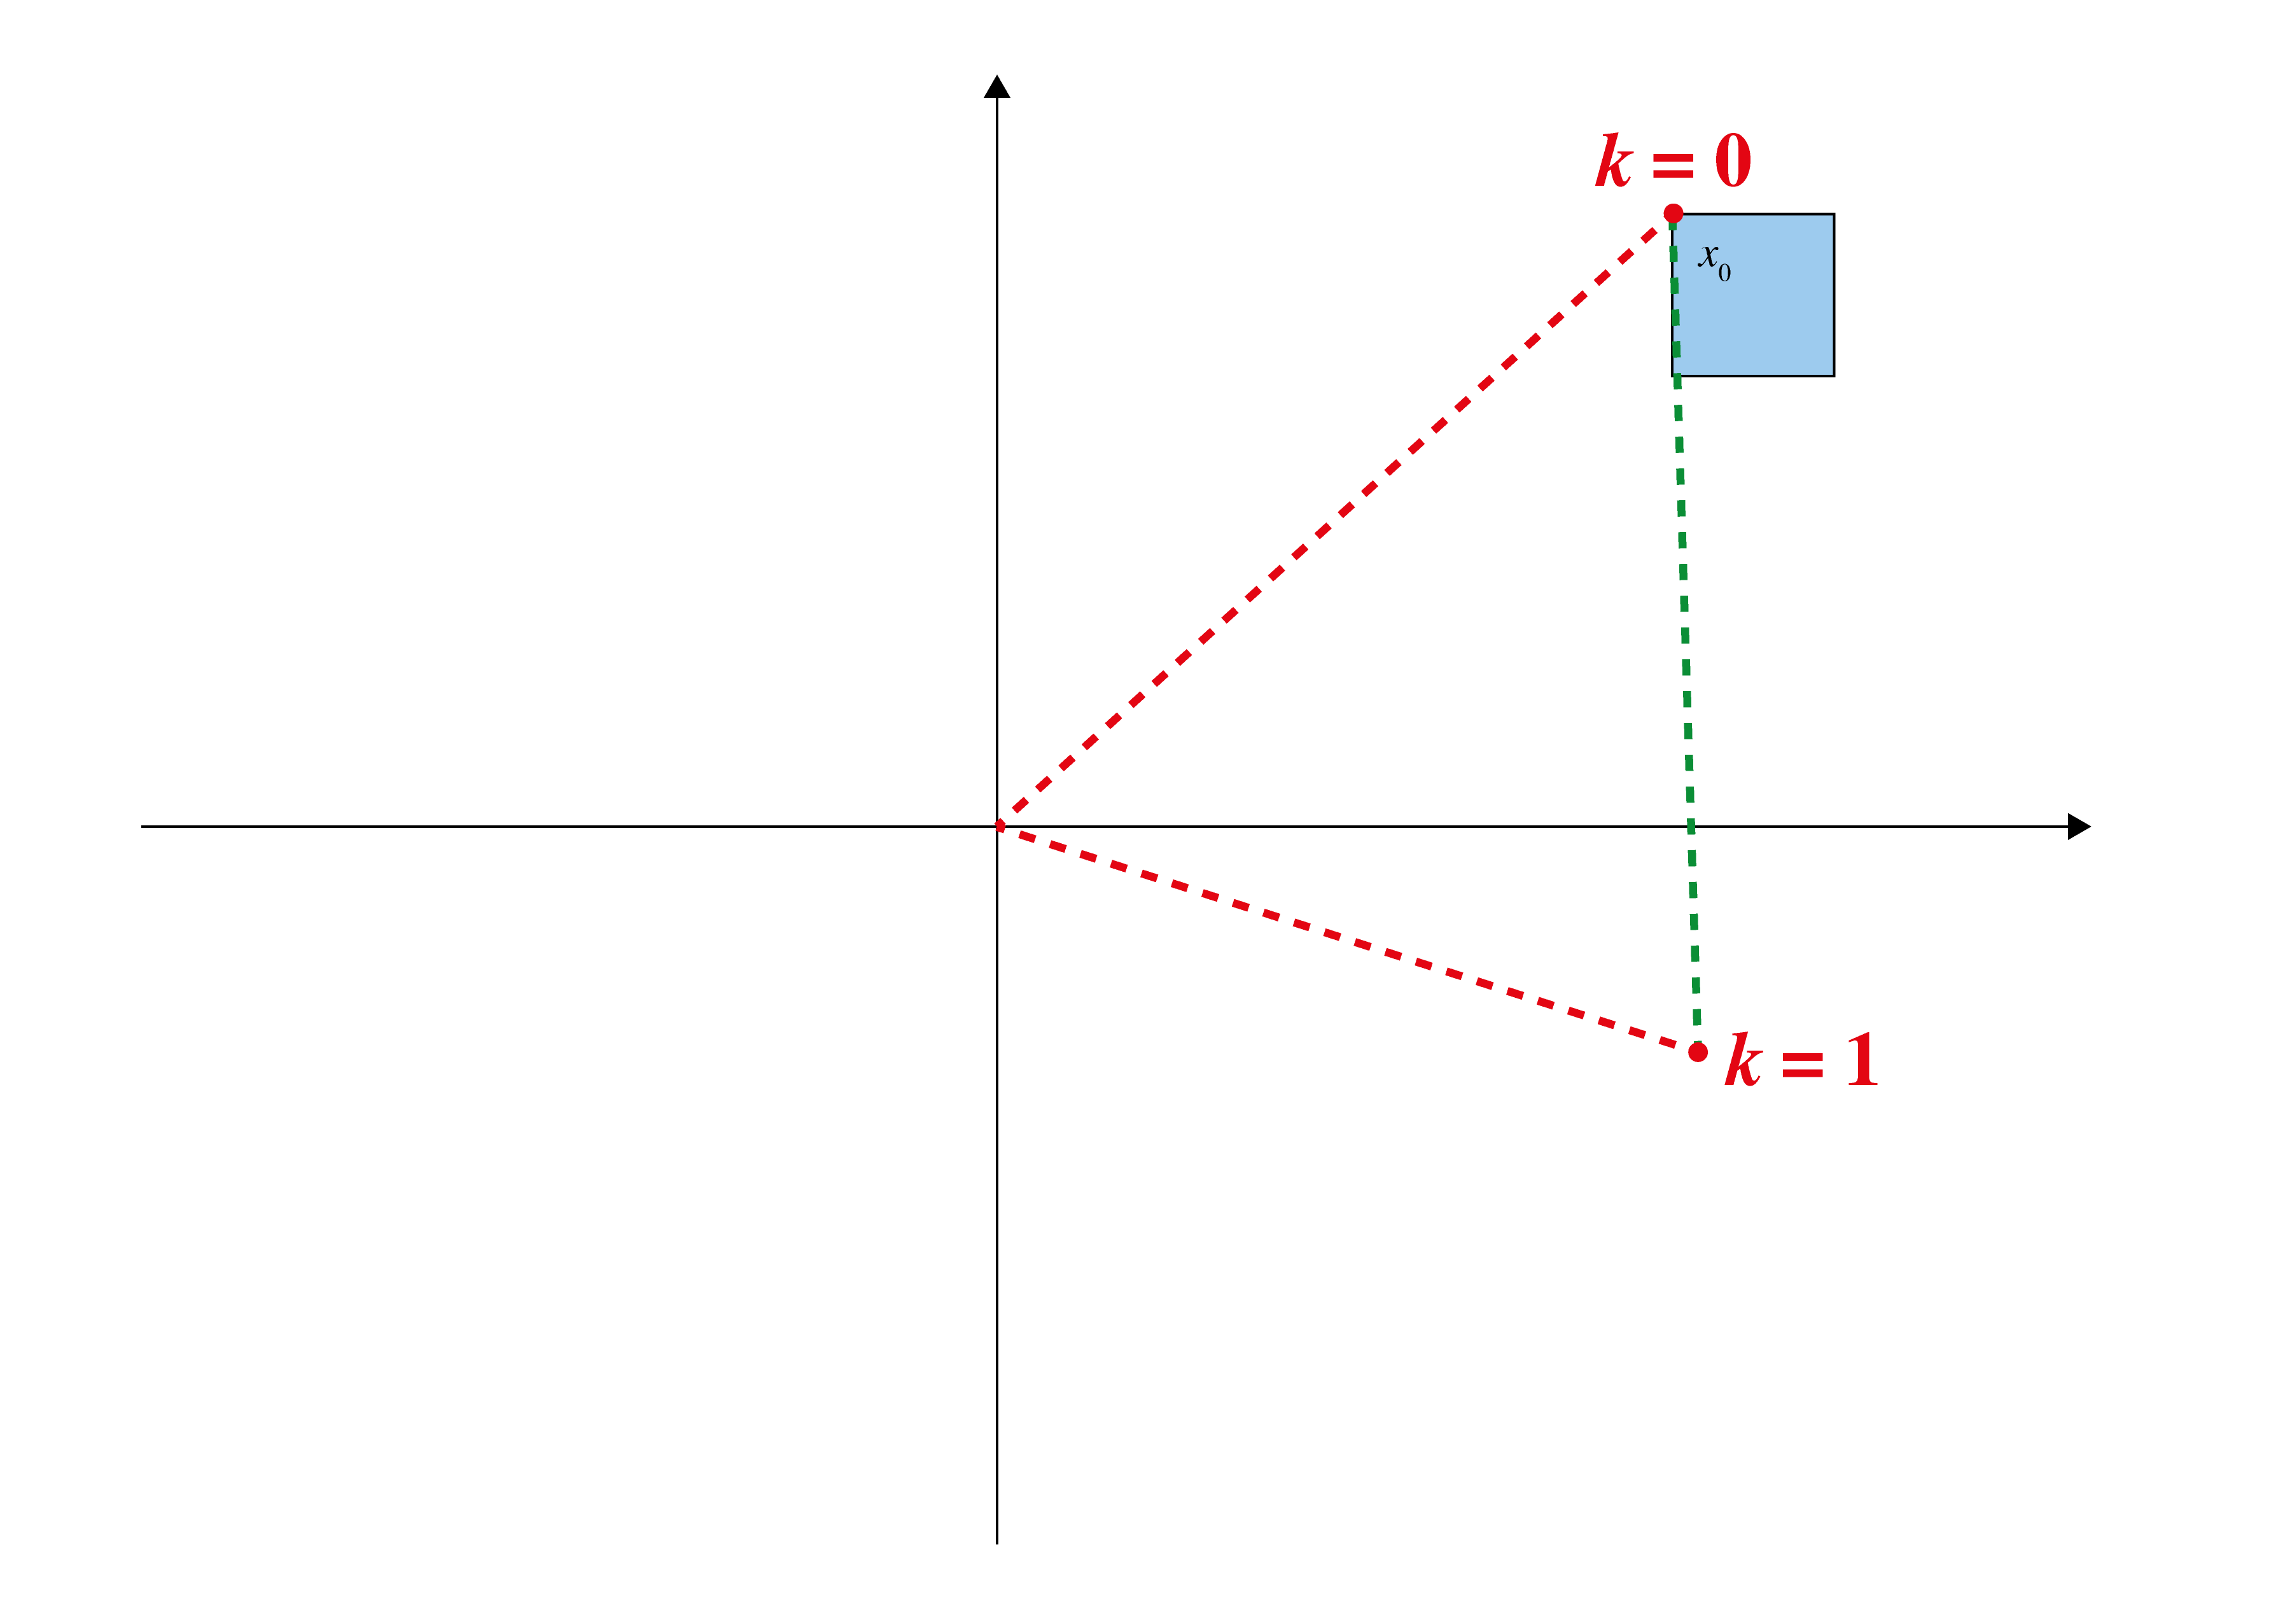
\includegraphics[width=.65\textwidth]{figures/spirals/Spirals-22.png}}
  \onslide<4>
  \centerline{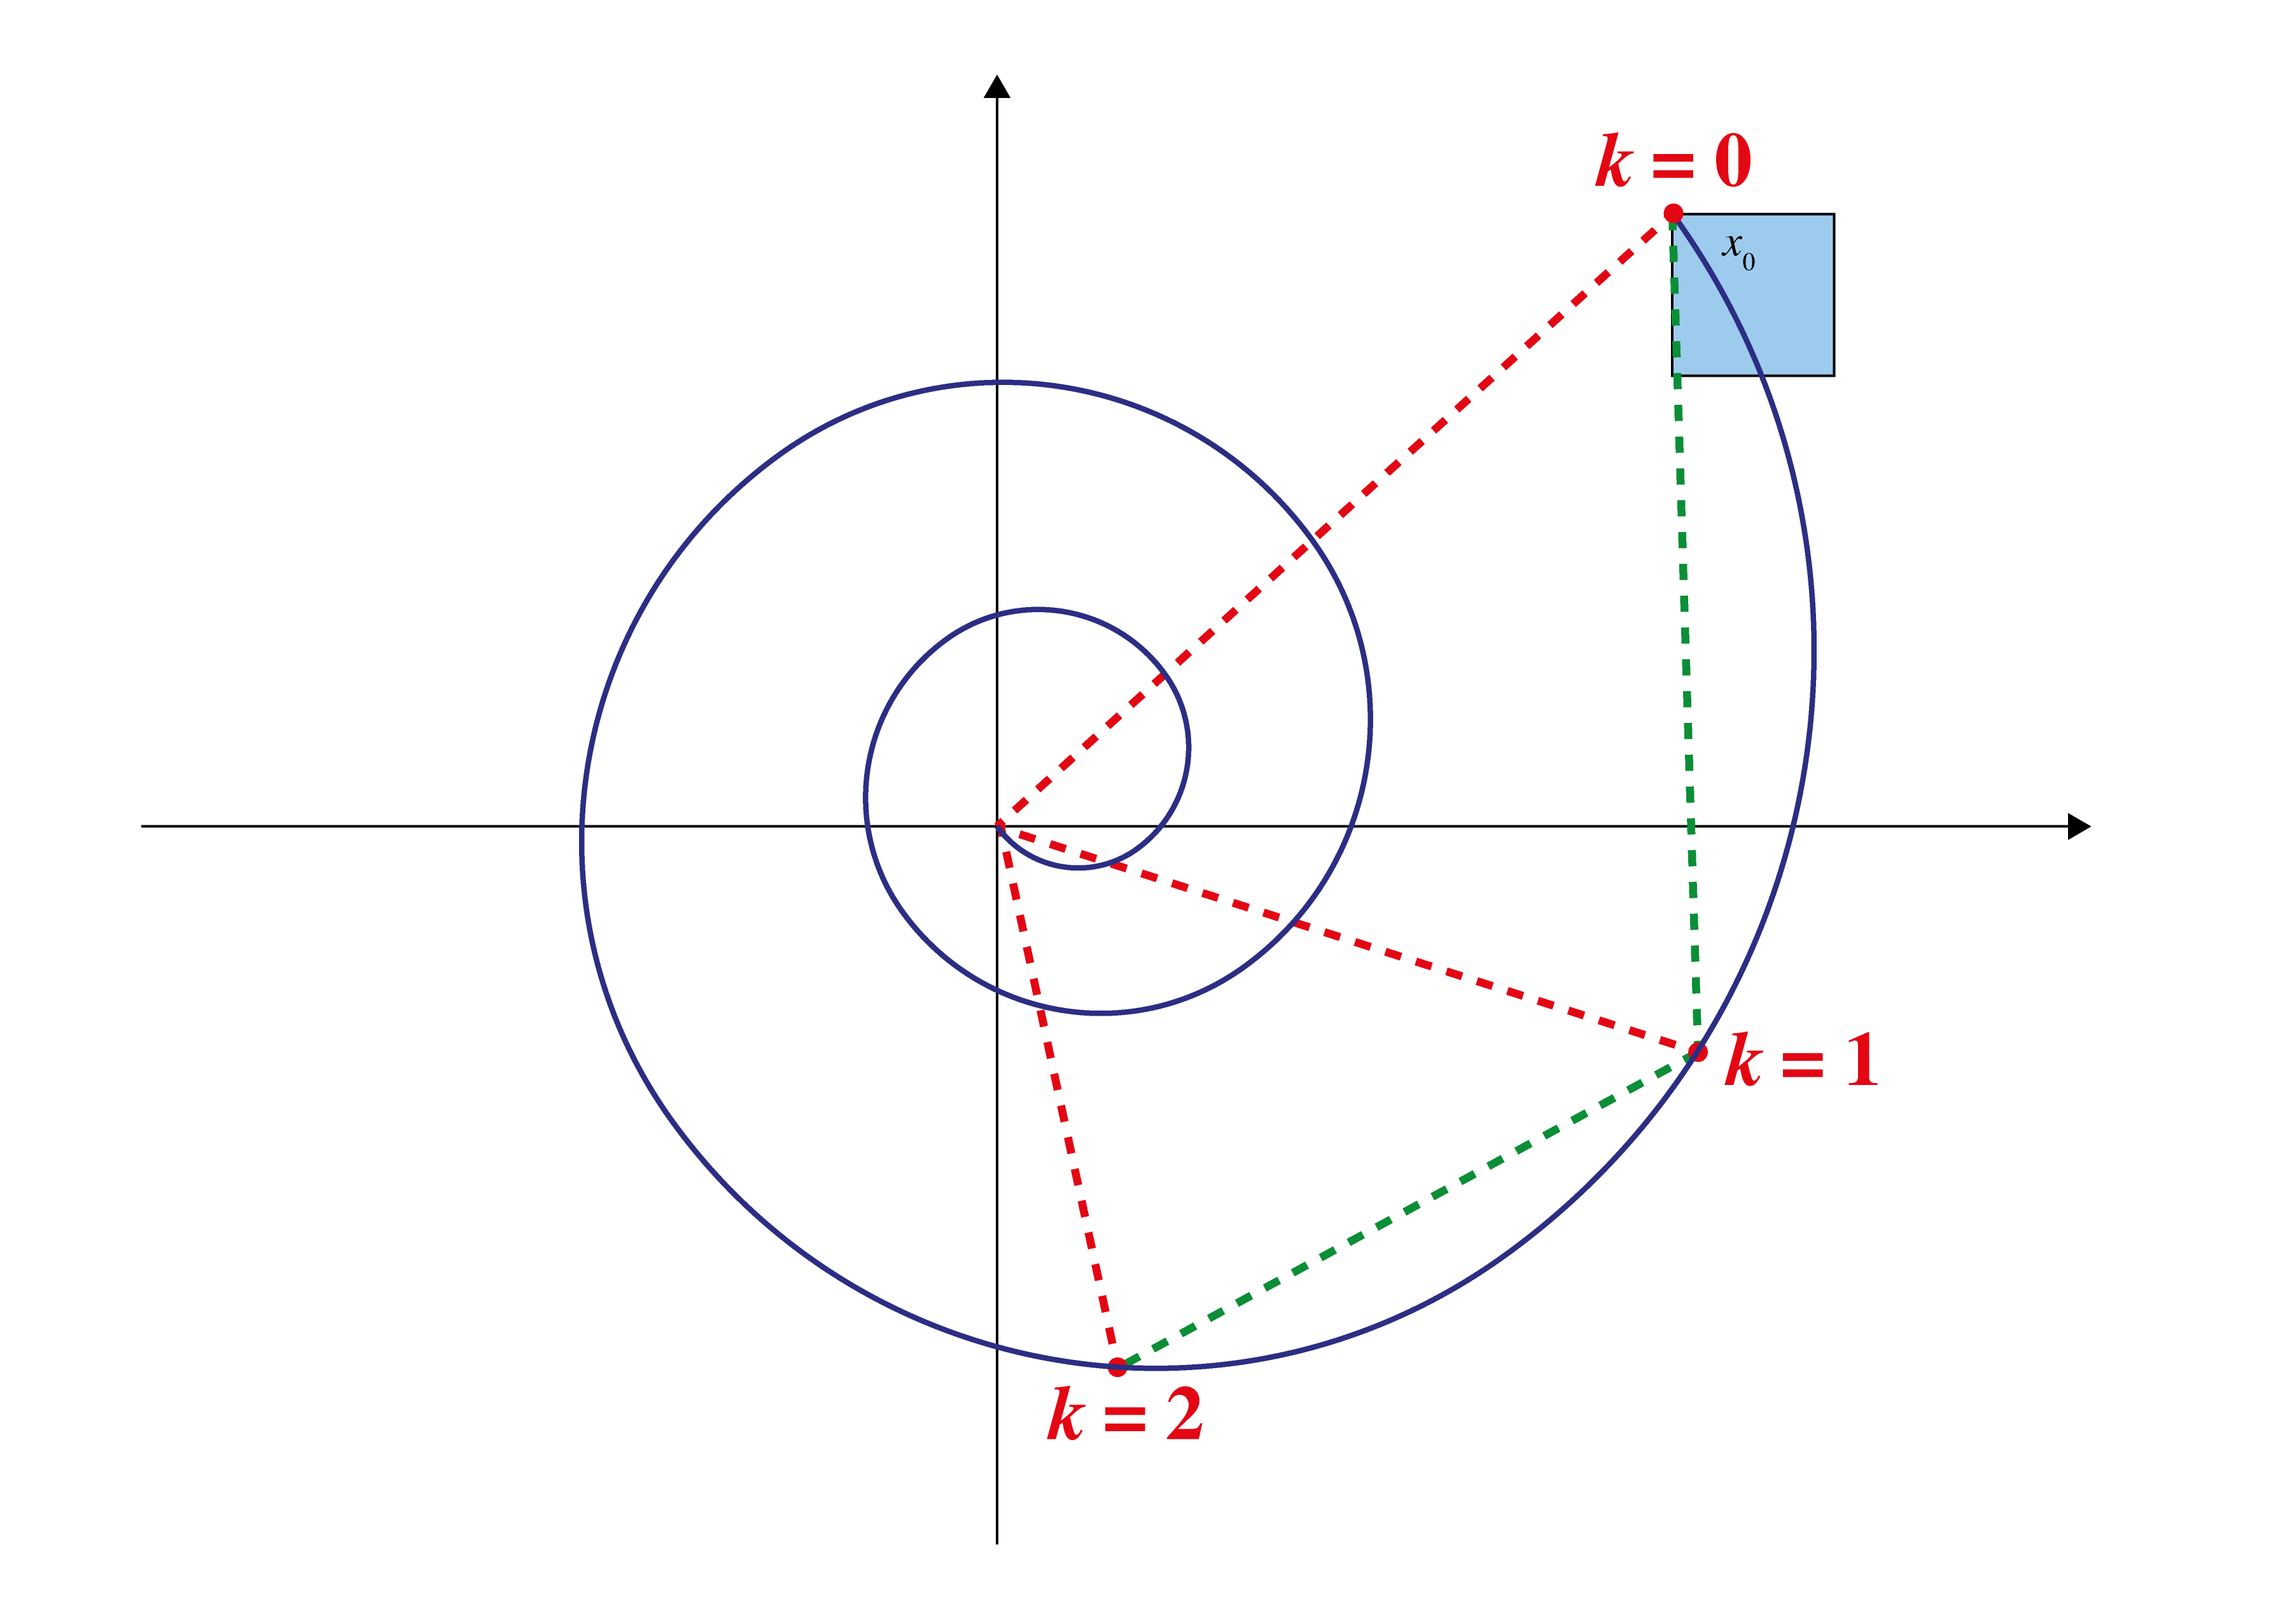
\includegraphics[width=.65\textwidth]{figures/spirals/Spirals-23.png}}
  \onslide<5>
  \centerline{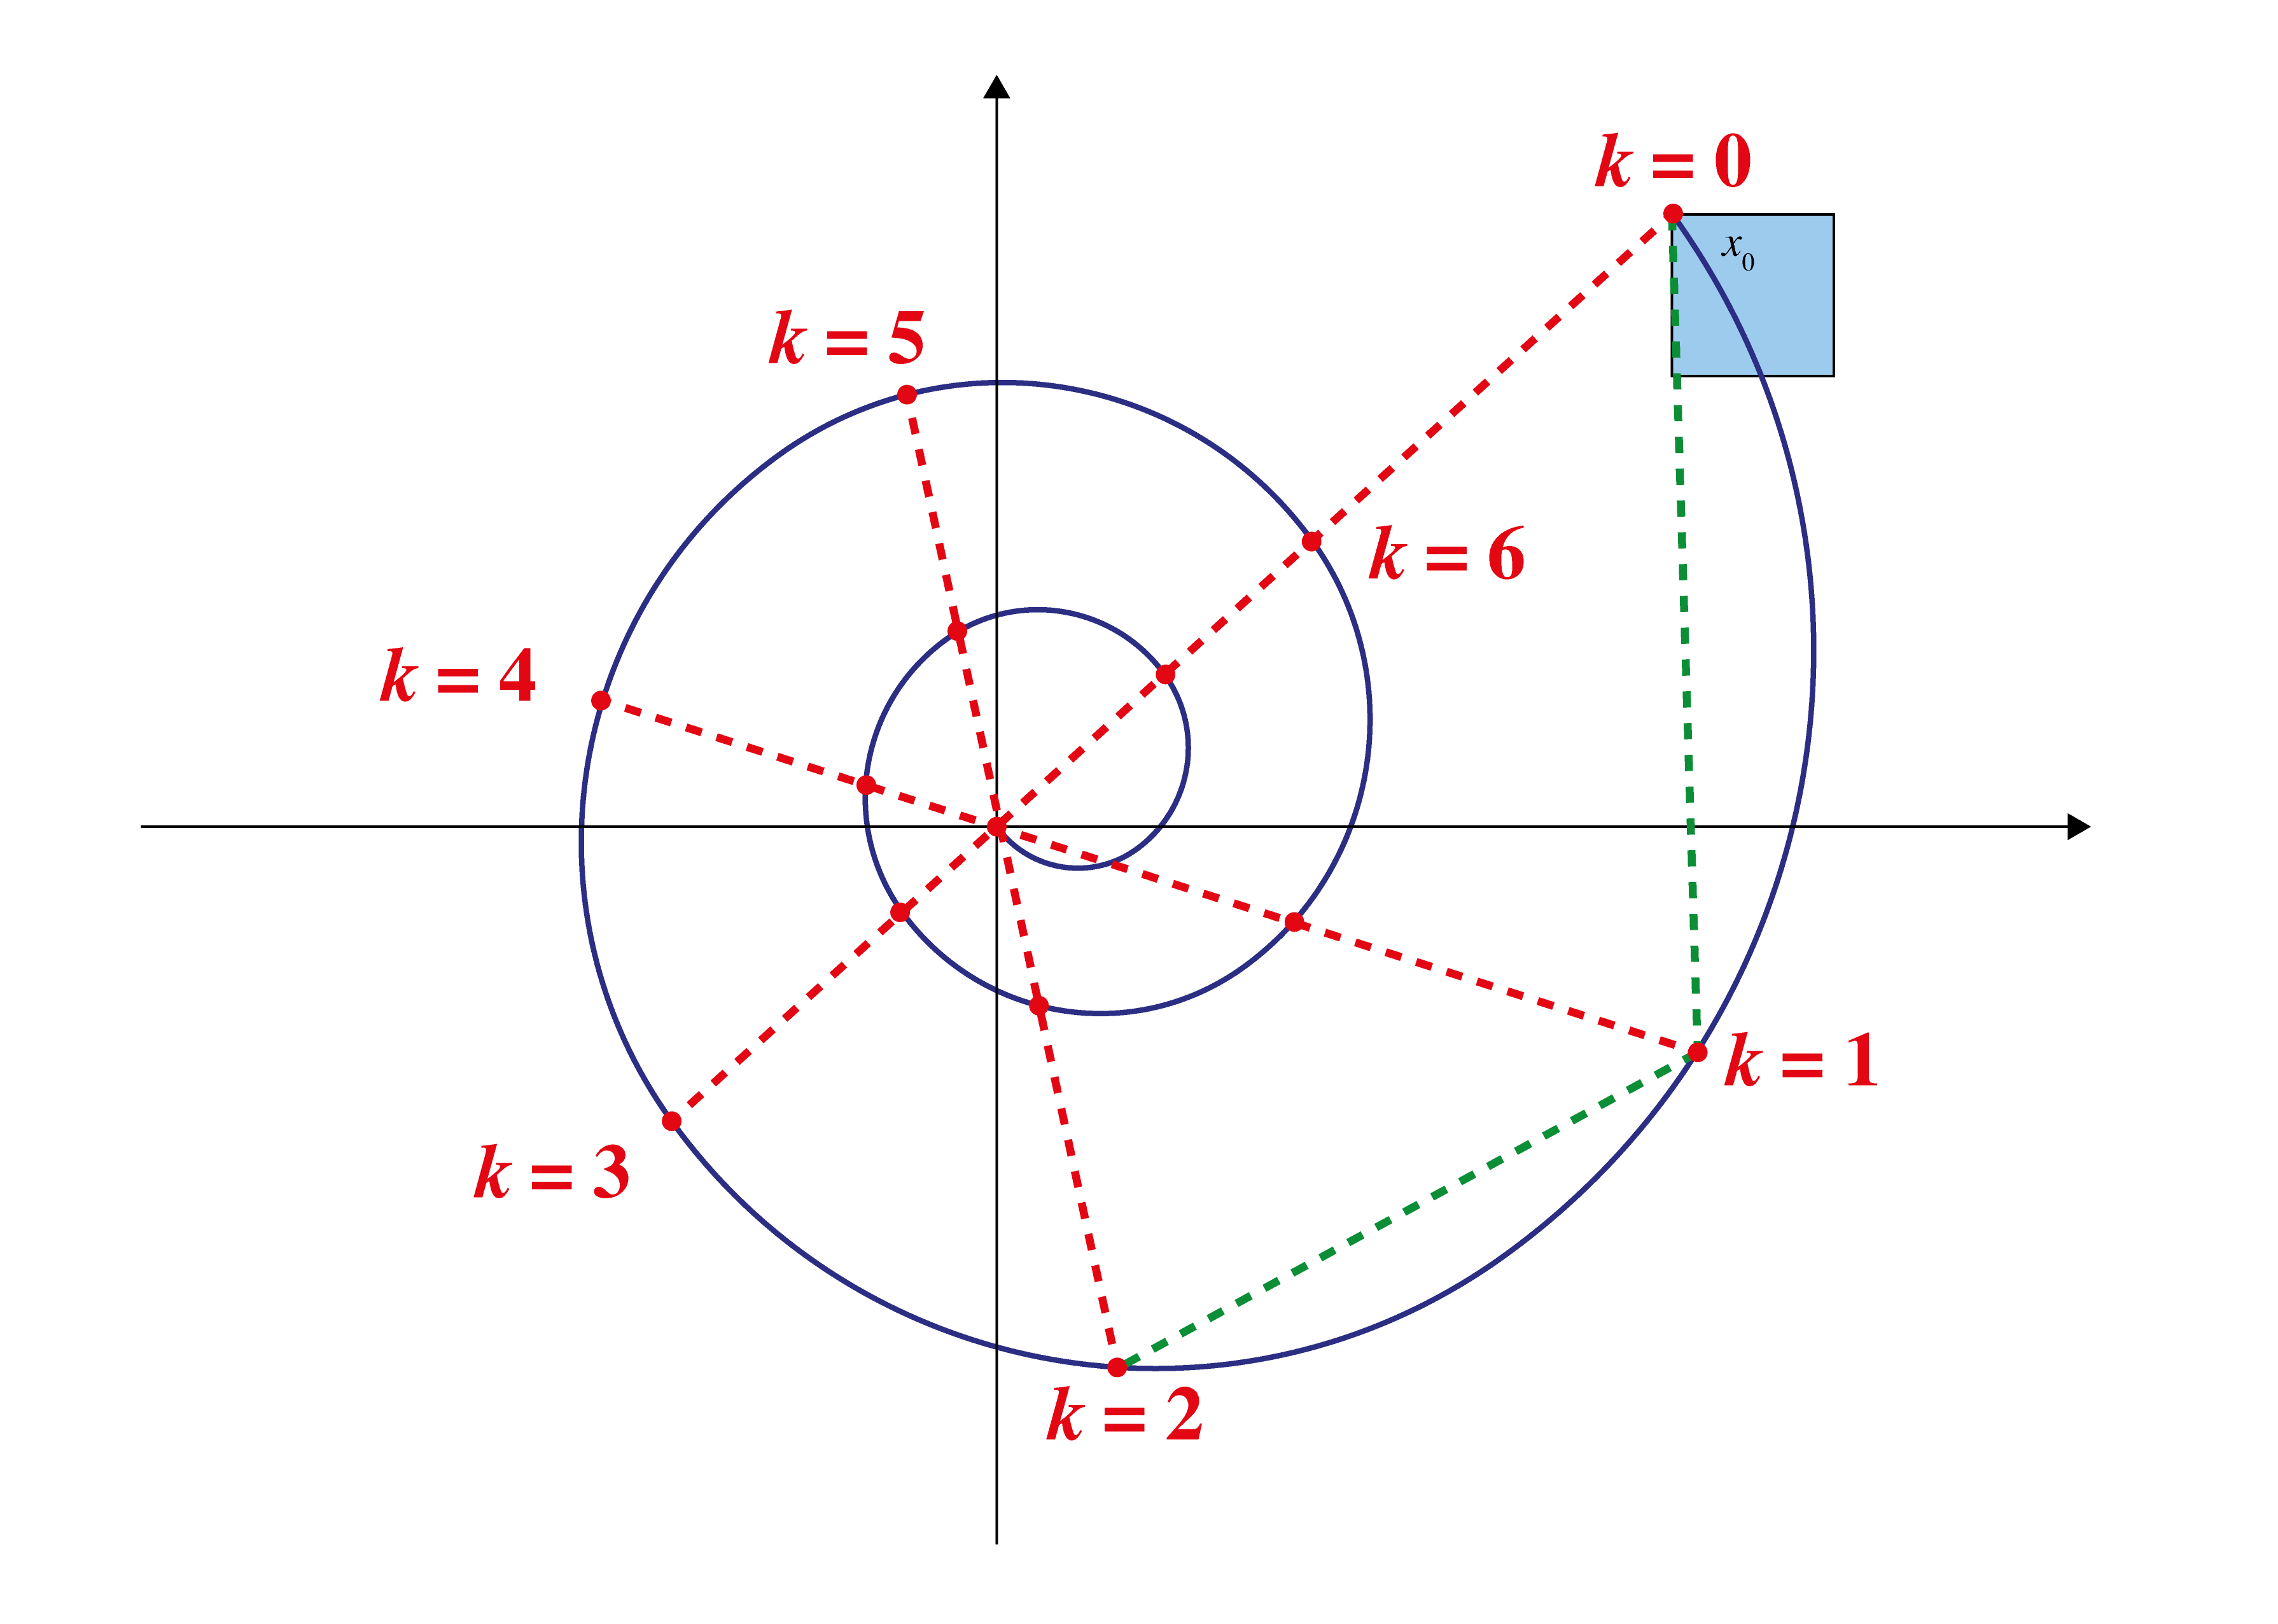
\includegraphics[width=.65\textwidth]{figures/spirals/Spirals-24.png}}
  \onslide<6>
  \centerline{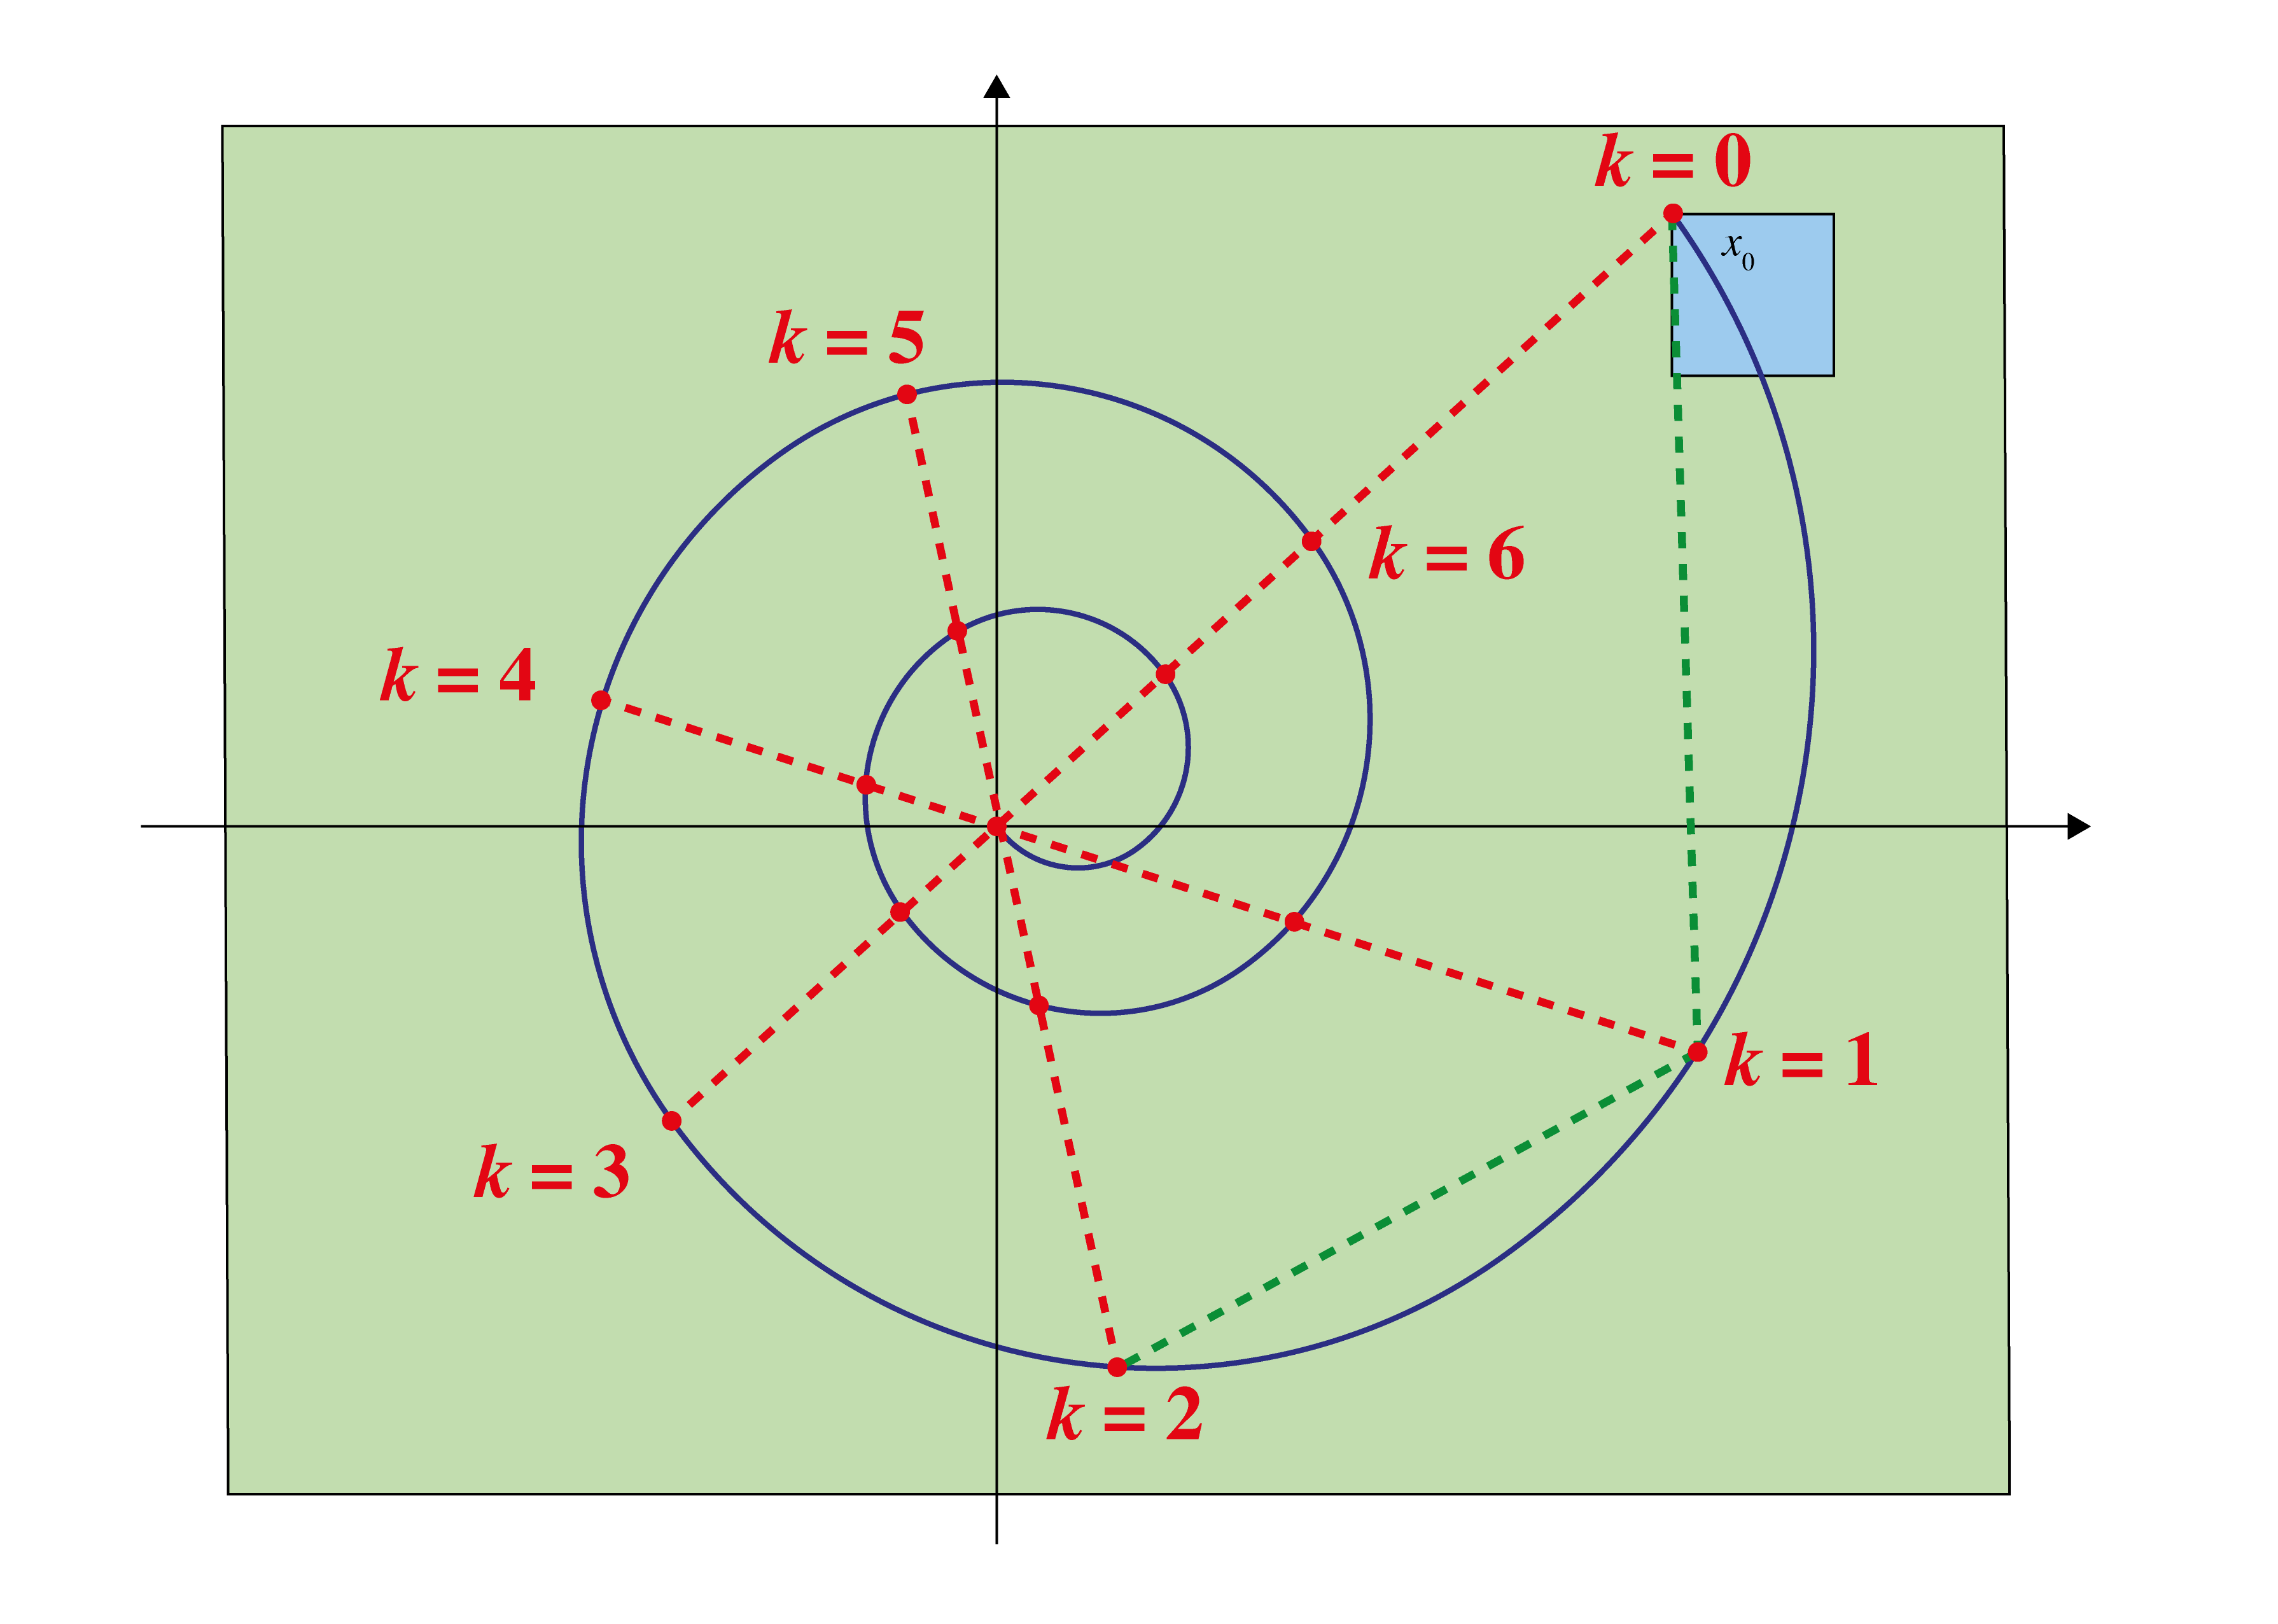
\includegraphics[width=.65\textwidth]{figures/spirals/Spirals-25.png}}
\end{overprint}
\end{center}

\end{frame}

%% \defverbatim[colored]\lstI{
%% \begin{lstlisting}[language=C++,basicstyle=\ttfamily,keywordstyle=\color{red}]
%% C=nondet;
%% [...]
%% \end{lstlisting}
%% }


\begin{frame}{Controller synthesis} 
\vspace{-.5cm}
 \centering 
 {\scriptsize
\resizebox{.65\textwidth}{!}
{
 \begin{tikzpicture}[scale=0.3,->,>=stealth',shorten >=.2pt,auto, semithick, initial text=, ampersand replacement=\&,]
  \matrix[nodes={draw, fill=none, shape=rectangle, minimum height=.2cm, minimum width=.2cm, align=center
},
          row sep=.6cm, column sep=.9cm] {
   \coordinate (aux1);
   \& \coordinate (aux2);
   \&;\\
   \coordinate (aux3);
   \& \coordinate (aux4);
   \&;\\
   \coordinate (aux5);
   \& \coordinate (aux6);
   \&;\\
   \node[minimum width=1.5cm, minimum height=0.6cm, fill=gray!20] (synth) {{\sc 1.Synthesize}};
   \only<2-7,9>{\node[minimum width=1.5cm, minimum height=0.6cm, fill=red!20] (synth) {{\sc 1.Synthesize}};}
   \&
   complexnode/.pic={ 
     \node[rectangle,draw,dotted,
	minimum width=6cm,
	minimum height=1cm,
        pattern=north west lines, pattern color=gray!20,
	label={\sc ~~~~~~~~~~~~Verify},] (verif) {};
     \node[minimum width=1cm, minimum height=0.6cm, fill=gray!20] (verif1) at ([xshift=-2cm]verif.center) {{\sc 2.Safety}};
     \only<8,10>{\node[minimum width=1cm, minimum height=0.6cm, fill=red!20] (verif1) at ([xshift=-2cm]verif.center) {{\sc 2.Safety}};}
     \node[minimum width=1cm, minimum height=0.6cm, fill=gray!20] (verif2) at ([xshift=0cm]verif.center) {{\sc 3.Precision}};
     \only<11>{\node[minimum width=1cm, minimum height=0.6cm, fill=red!20] (verif2) at ([xshift=0cm]verif.center) {{\sc 3.Precision}};}
     \node[minimum width=1cm, minimum height=0.6cm, fill=gray!20] (verif3) at ([xshift=2cm]verif.center) {{\sc 4.Complete}};
     \only<12>{\node[minimum width=1cm, minimum height=0.6cm, fill=red!20] (verif3) at ([xshift=2cm]verif.center) {{\sc 4.Complete}};}
   } 
   \& \node[ellipse, fill=gray!20] (done) {{\sc Done}};
   \only<13>{\node[ellipse, fill=red!20] (done) {{\sc Done}};}\\
   \& \\
   %% \node[minimum height=0cm] (gp) {\sf Program Search};
   %% \&
   %% complexnode/.pic={ 
   %%   \coordinate (aux);
   %% \node (bmc) at ([xshift=-2cm]aux.center) {\sf BMC-based \\ \sf Verifier};
   %% \node (fp)  at ([xshift=0cm]aux.center) {\sf Fixed-point \\ \sf Arithmetic\\ \sf Verifier};
   %% \node (sv)  at ([xshift=2cm]aux.center) {\sf Completeness\\ \sf Verifier};
   %% }   
   %%  \\
  };

   \path
    ([yshift=2em]synth.east) edge node[xshift=-0.5em,align=center] {$C$} ([yshift=2em]verif1.west)
    ([yshift=-2em]verif1.west) edge node {C-ex} ([yshift=-2em]synth.east)
%    ([xshift=-5em]fp.north) edge node[align=center]  {} ([xshift=-5em]verif2.south)
%    ([xshift=-5em]sv.north) edge node[align=center]  {} ([xshift=-5em]verif3.south)
%    ([xshift=5em]verif1.south) edge node[align=center] {} ([xshift=5em]bmc.north)
 %   ([xshift=5em]verif2.south) edge node[align=center] {} ([xshift=5em]fp.north)
%    ([xshift=5em]verif3.south) edge node[align=center] {} ([xshift=5em]sv.north)
%    ([xshift=-5em]bmc.north) edge node[align=center]  {} ([xshift=-5em]verif1.south)
    (verif) edge node {PASS} (done)
    %% ([xshift=5em]synth.south) edge node[align=center] {} ([xshift=5em]gp.north)
    %% ([xshift=-5em]gp.north) edge node[align=center] {} ([xshift=-5em]synth.south)
    (aux3) edge (synth.north);
   \path[-]
   (verif2.north) edge node[align=center] {} ([xshift=0cm]aux6)
   ([xshift=0cm]aux6) edge node[align=center] {Increase Precision} (aux5)
   (verif3.north) edge node[align=center] {} ([xshift=6.7cm]aux4)
   ([xshift=6.7cm]aux4) edge node[align=center] {Increase Unfolding Bound} (aux3);
 \end{tikzpicture}
}}

 \scriptsize
 %&
 \begin{tabular}{p{\dimexpr 0.5\linewidth-2\tabcolsep} 
     p{\dimexpr 0.5\linewidth-2\tabcolsep}}

   \only<2-7>{
     \begin{tabular}{l}
       {\bf Find a controller for given $\{x_0\}$ and $k{=}6$} \\
       {\bf such that the system is stable and safe} \\
     \\\\\\\\\\\\\\\\\\\\\\\\\\
  \end{tabular}
   }
   \only<8>{
     \begin{tabular}{l}
       {\bf Find an initial state for which the system}\\
       {\bf is unsafe} \\
     \\\\\\\\\\\\\\\\\\\\\\\\\\
  \end{tabular}
   }
   \only<9>{
     \begin{tabular}{l}
       {\bf Find a controller for $\{x_0, x_0'\}$ and $k{=}6$}\\
       {\bf such that the system is stable and safe} \\
     \\\\\\\\\\\\\\\\\\\\\\\\\\
  \end{tabular}
   }
   \only<10>{
     \begin{tabular}{l}
       {\bf Find an initial state for which the system}\\
       {\bf is unsafe} \\       
     \\\\\\\\\\\\\\\\\\\\\\\\\\     
  \end{tabular}
   }
   \only<11>{
     \begin{tabular}{l}
     {\bf Check that the plant precision is sufficient}\\
     \\\\\\\\\\\\\\\\\\\\\\\\\\\\     
  \end{tabular}
   }
   \only<12>{
     \begin{tabular}{l}
       {\bf Check that $k$ is sufficient} \\
     \\\\\\\\\\\\\\\\\\\\\\\\\\\\     
  \end{tabular}
   }
   \only<13>{
     \begin{tabular}{l}
       {\bf Controller found}\\
     \\\\\\\\\\\\\\\\\\\\\\\\\\\\     
  \end{tabular}
   }
 
   &
   \begin{overprint}
   \onslide<2,3,4,5,6>
       \scalebox{0.65}{
   \hspace{1cm}
     \begin{minipage}{0.6\linewidth}
      \begin{algorithm}[H]
\begin{algorithmic}[1]
  \only<3>{\STATE \colorbox{red!20}{\textbf{Input:} $x_0$, $k$.}
        \STATE \colorbox{red!20}{\textbf{Output:} {\color {red} $C$}.}}
  \only<2,4->{\STATE \textbf{Input:} $x_0$, $k$.
          \STATE \textbf{Output:} {\color {red} $C$}.}
  \only<2,3,5->{\STATE {\color {red} $C$}=nondet;
        \STATE \textbf{assume}({\color {black} \textbf{STABLE}}(A,B,{\color {red} $C$}));}
  \only<4>{\STATE \colorbox{red!20}{{\color {red} $C$}=nondet;}
  \STATE \colorbox{red!20}{\textbf{assume}(\textbf{STABLE}(A,B,{\color {red} $C$}));}}
  \only<1,2,3,4,6->{ \STATE \textbf{assume}(\textbf{SAFE}($x_{0}$));
    \STATE {$i=0$};
  \WHILE{$i<k$}
        \STATE $x_{i+1}=x_i(A-B{\color {red} C})$
        \STATE assume({\color {black} \textbf{SAFE}}($x_{i+1}$));
          \STATE $i=i+1$;}
  \only<5>{\STATE \colorbox{red!20}{\textbf{assume}(\textbf{SAFE}($x_{0}$));}
        \STATE \colorbox{red!20}{$i=0$};
  \WHILE{\colorbox{red!20}{$i<k$}}
        \STATE \colorbox{red!20}{$x_{i+1}=x_i(A-B{\color {red} C})$}
        \STATE \colorbox{red!20}{assume({\color {black} \textbf{SAFE}}($x_{i+1}$));}
          \STATE \colorbox{red!20}{$i=i+1$;}}
          \ENDWHILE
          \only<6>{\STATE \colorbox{red!20}{\textbf{assert}(false);}}
          \only<1,2,3,4,5>{\STATE \textbf{assert}(false);}
\end{algorithmic}
\caption*{\textsc{synthesize}}
\label{alg:seq}
\end{algorithm}
    \end{minipage}
    }
   

%% \begin{lstlisting}[mathescape,language=C++,basicstyle=\ttfamily,keywordstyle=\color{red},linewidth=5cm]
%%      function synthesise($x_0$,k)
%%        C=nondet;
%%        assume(Jury_criterion(C));
%%        x[0]=$x_0$
%%        k=1;
%%        while(k<6) {
%%          x[k+1]
%%      \end{lstlisting}

     \onslide<7>
     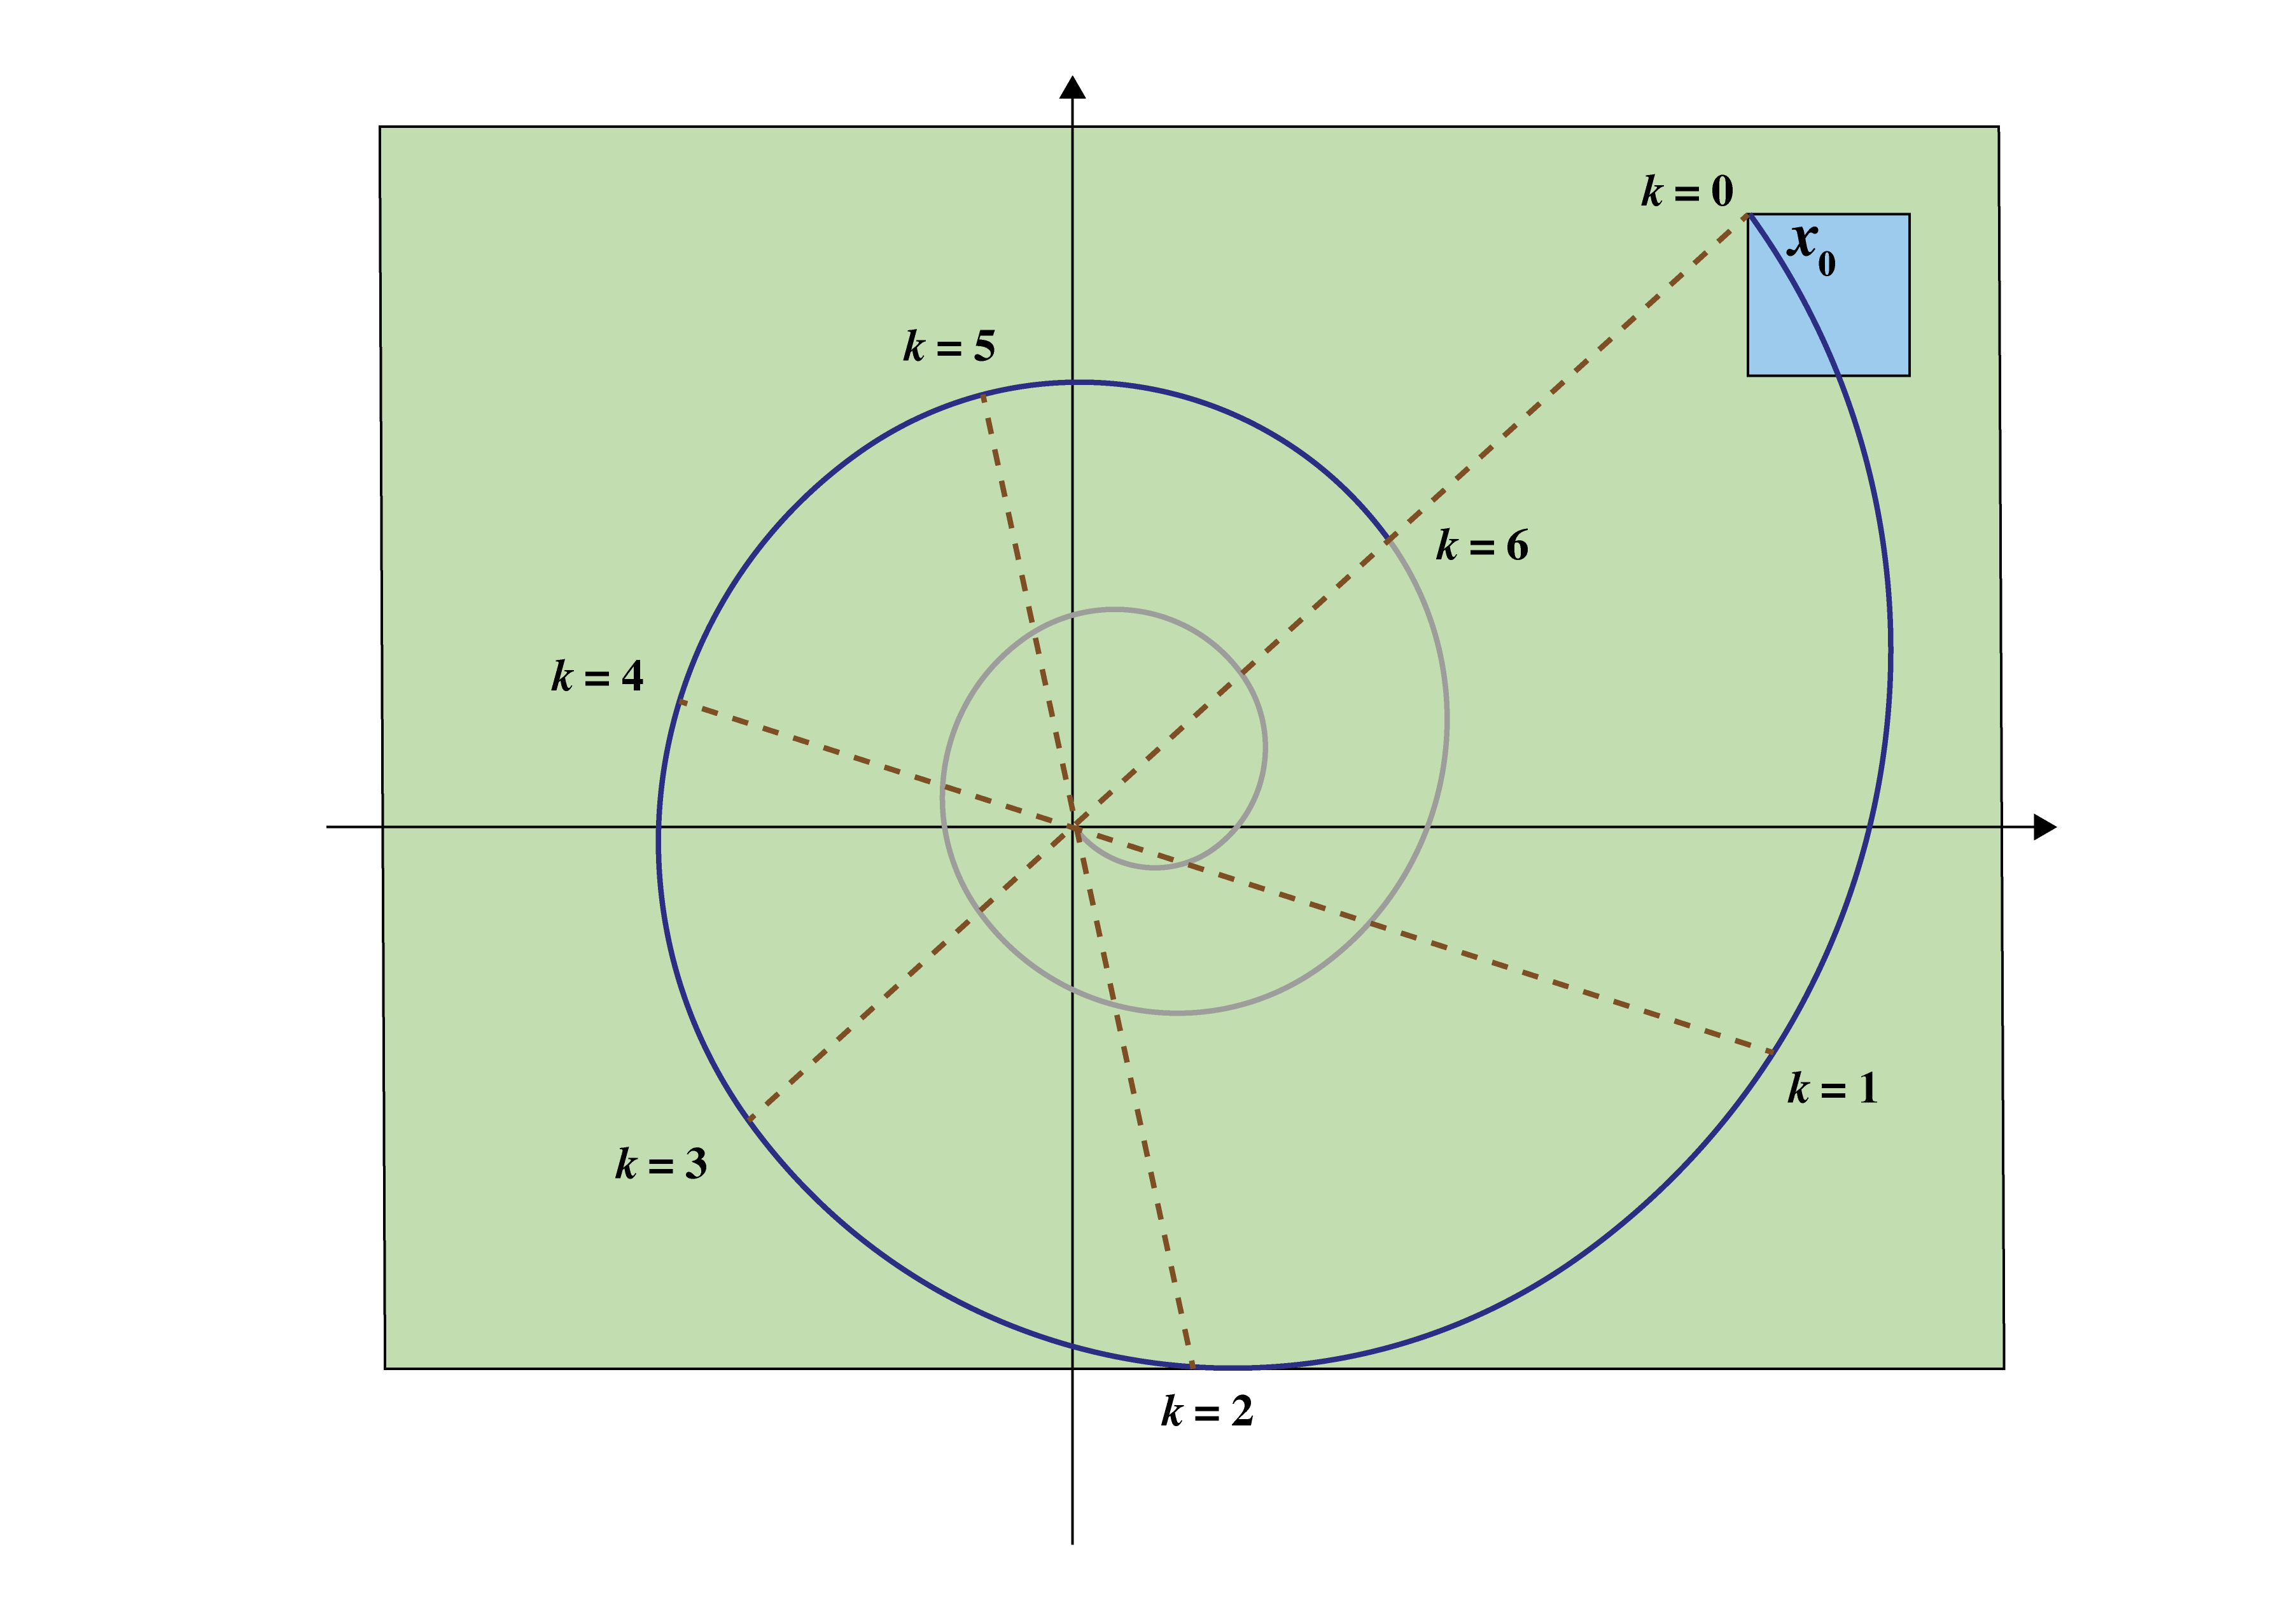
\includegraphics[width=.55\textwidth]{figures/spirals/Spirals-05.png}
     \onslide<8>
     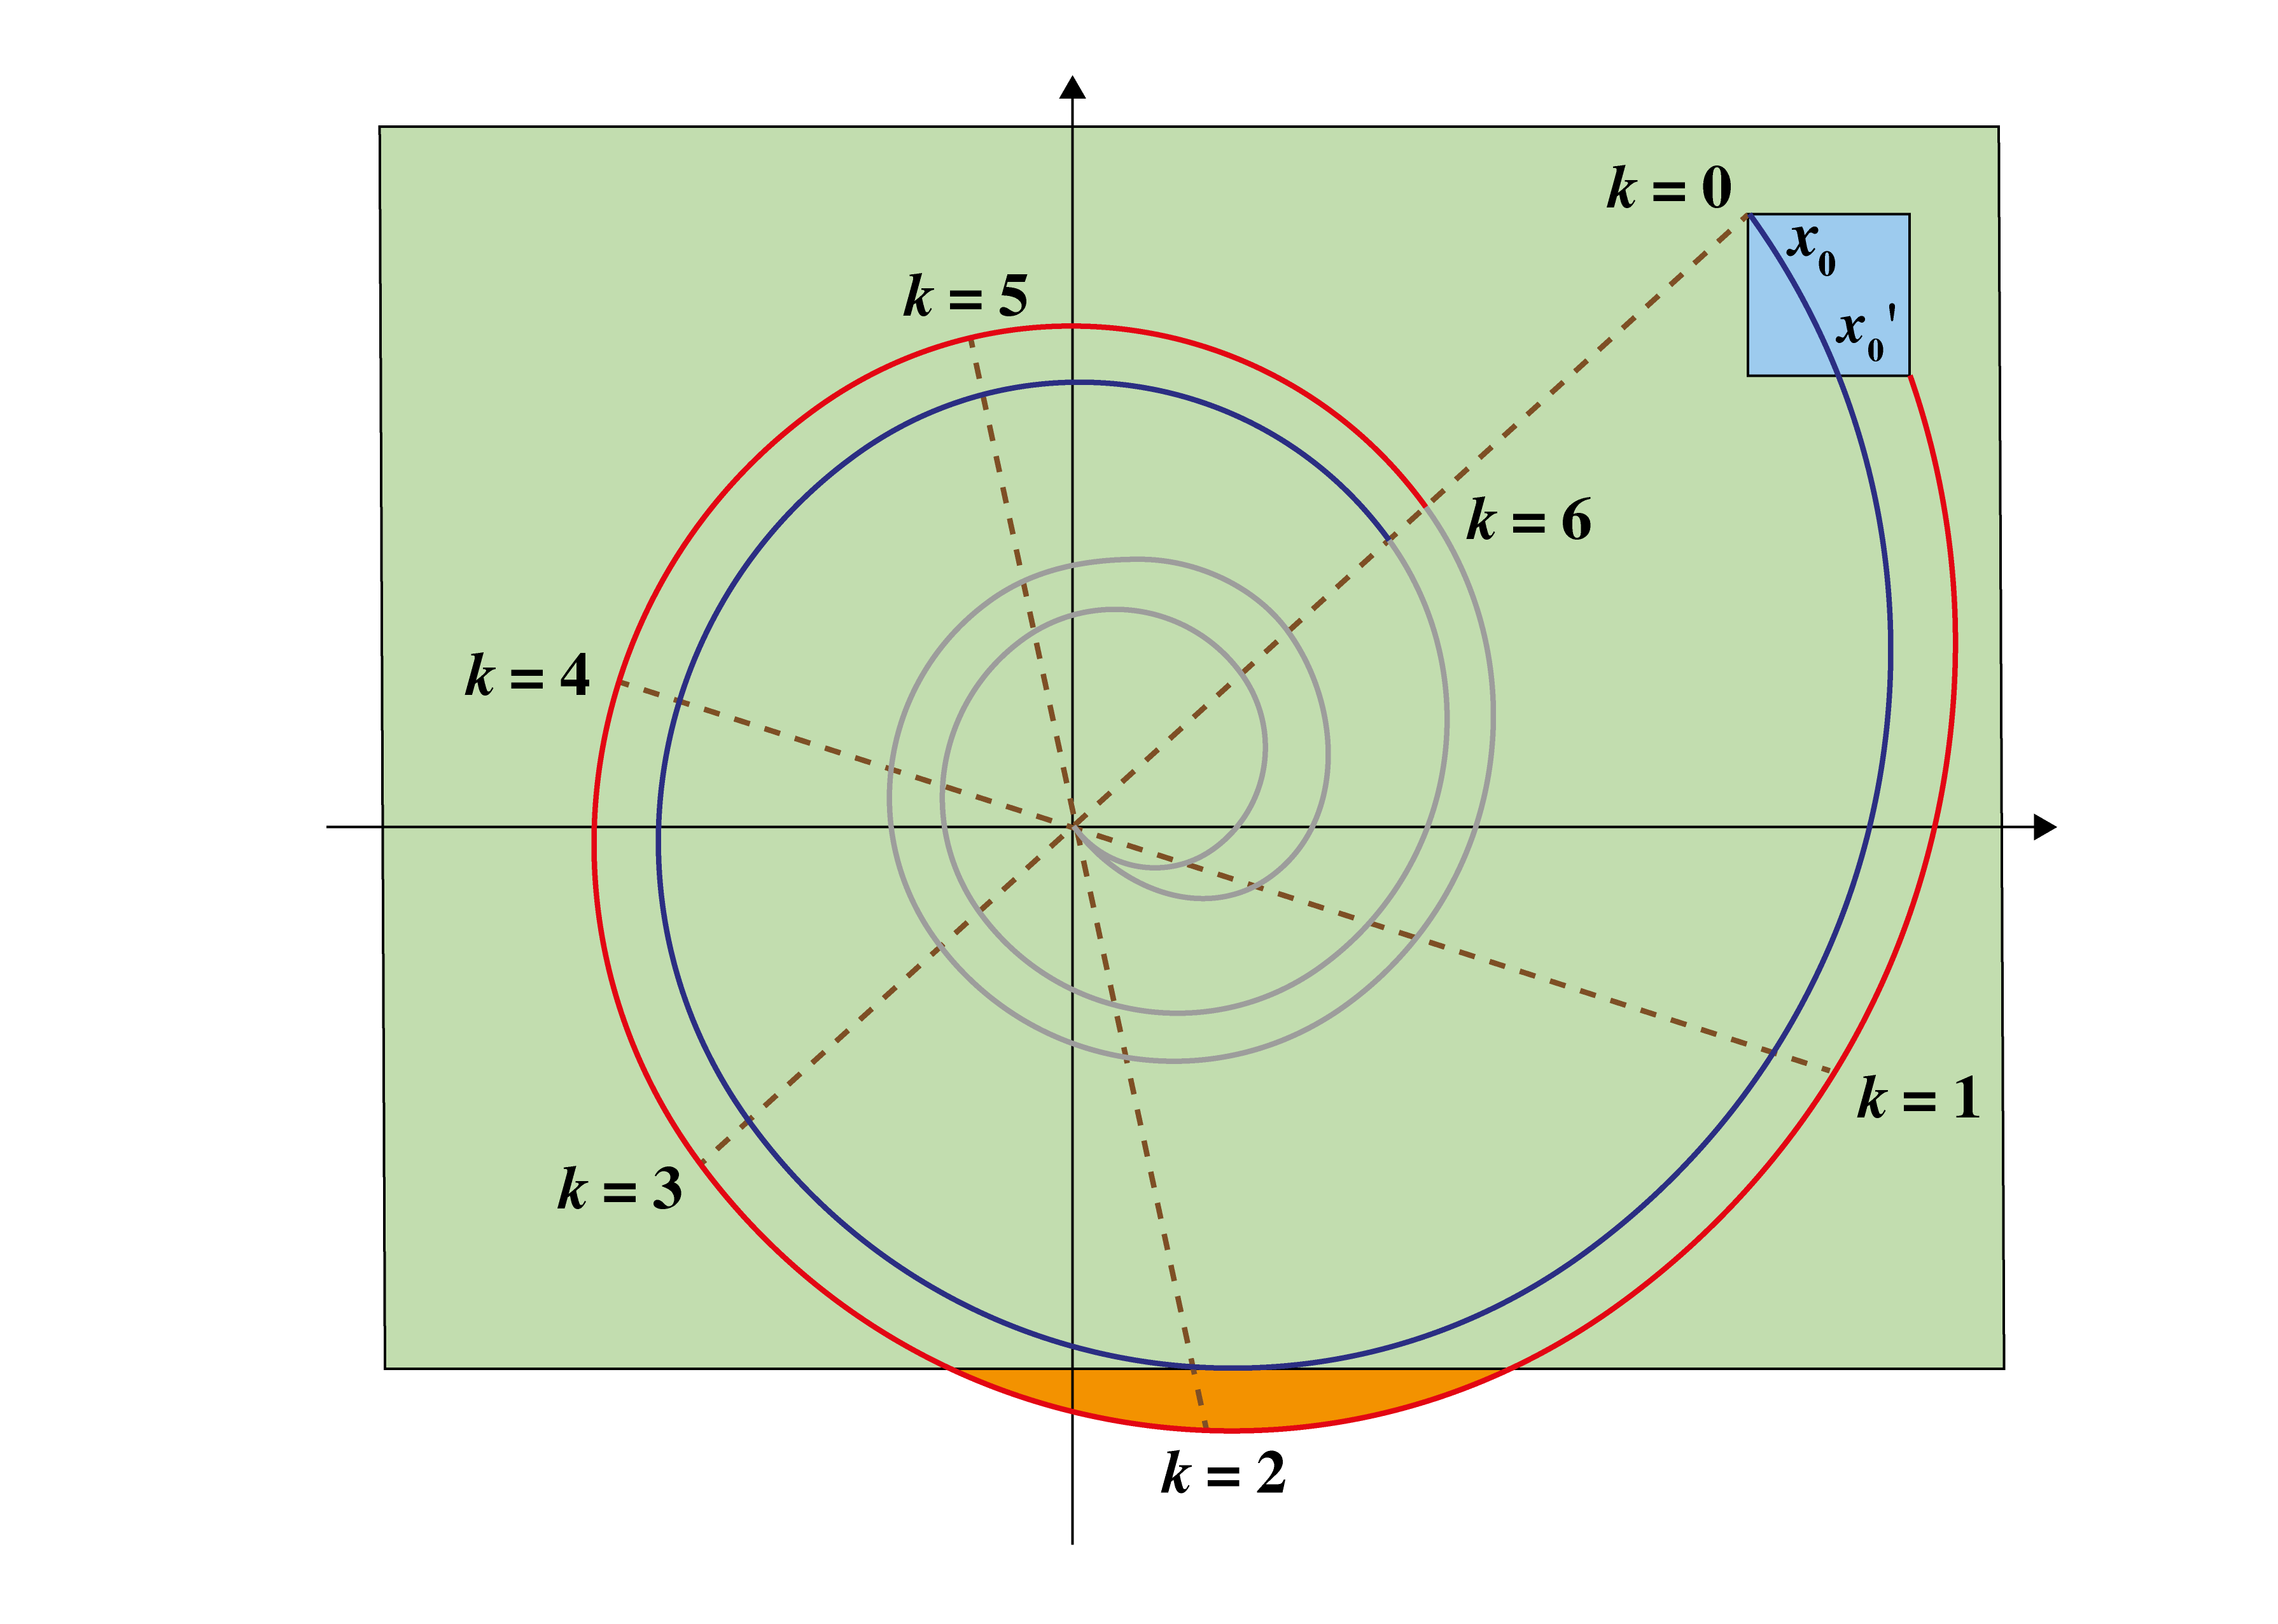
\includegraphics[width=.55\textwidth]{figures/spirals/Spirals-04.png}
     \onslide<9,10,11>
     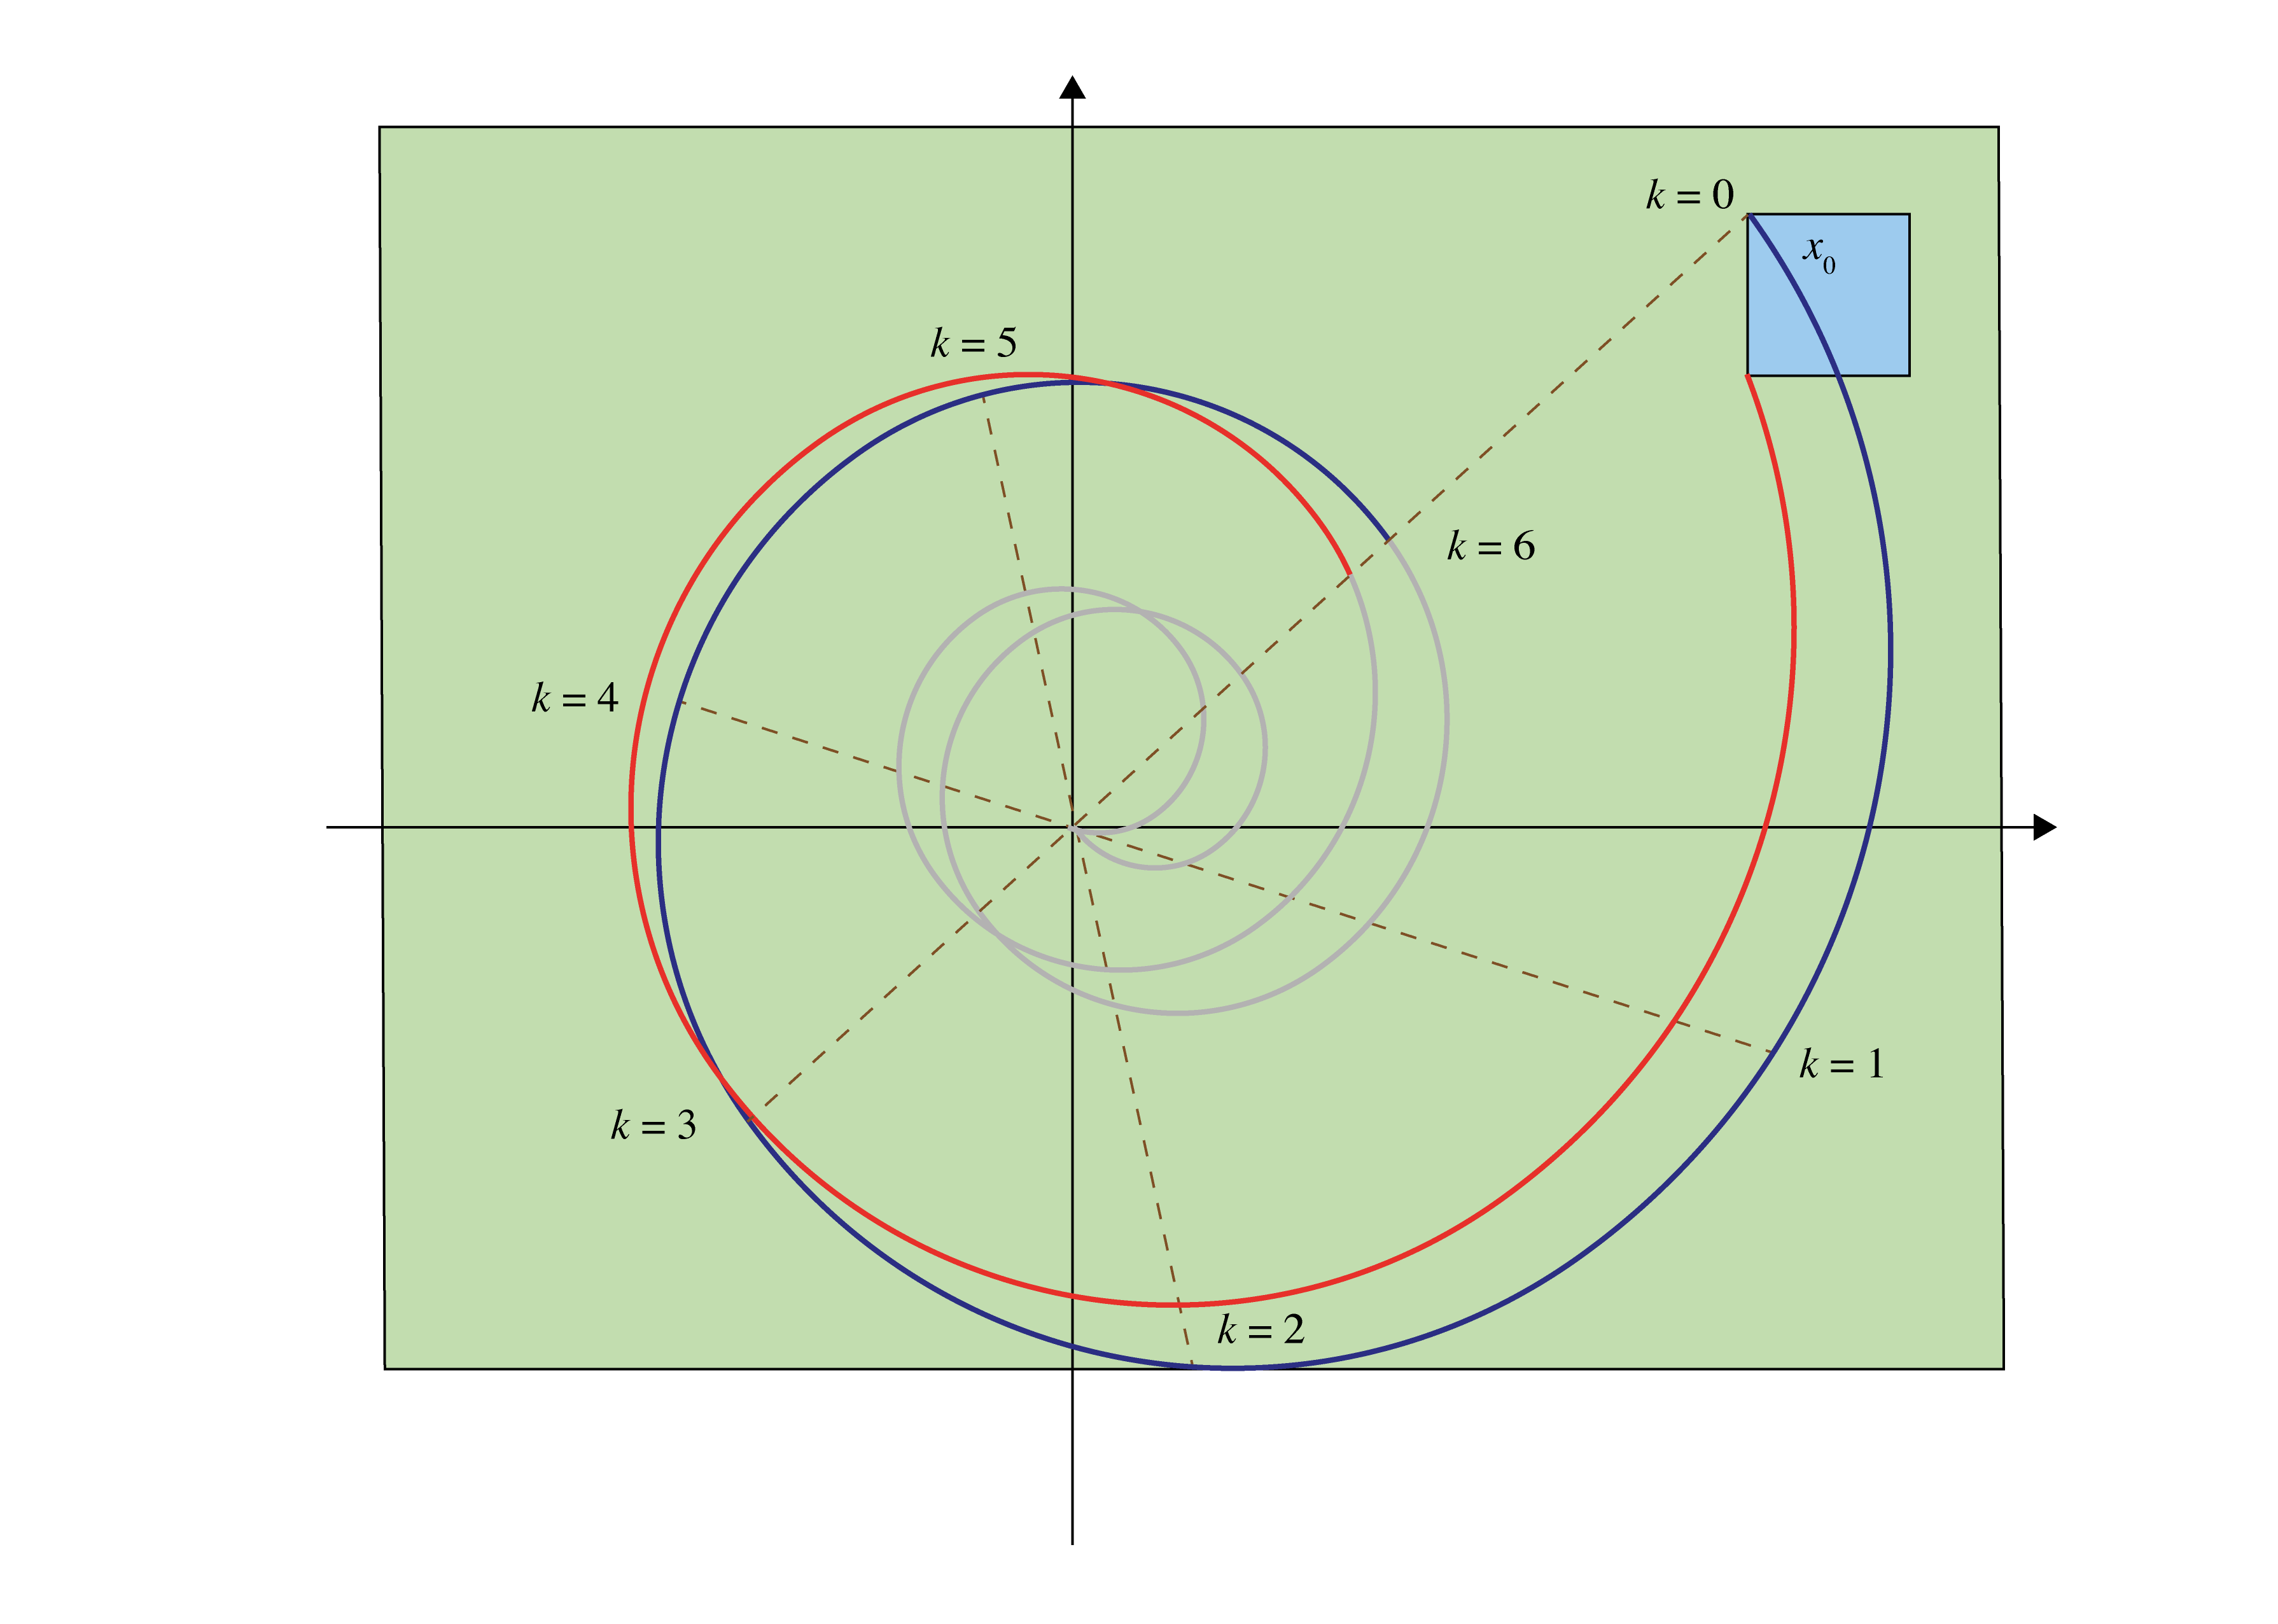
\includegraphics[width=.55\textwidth]{figures/spirals/Spirals-06.png}
     \onslide<12->
         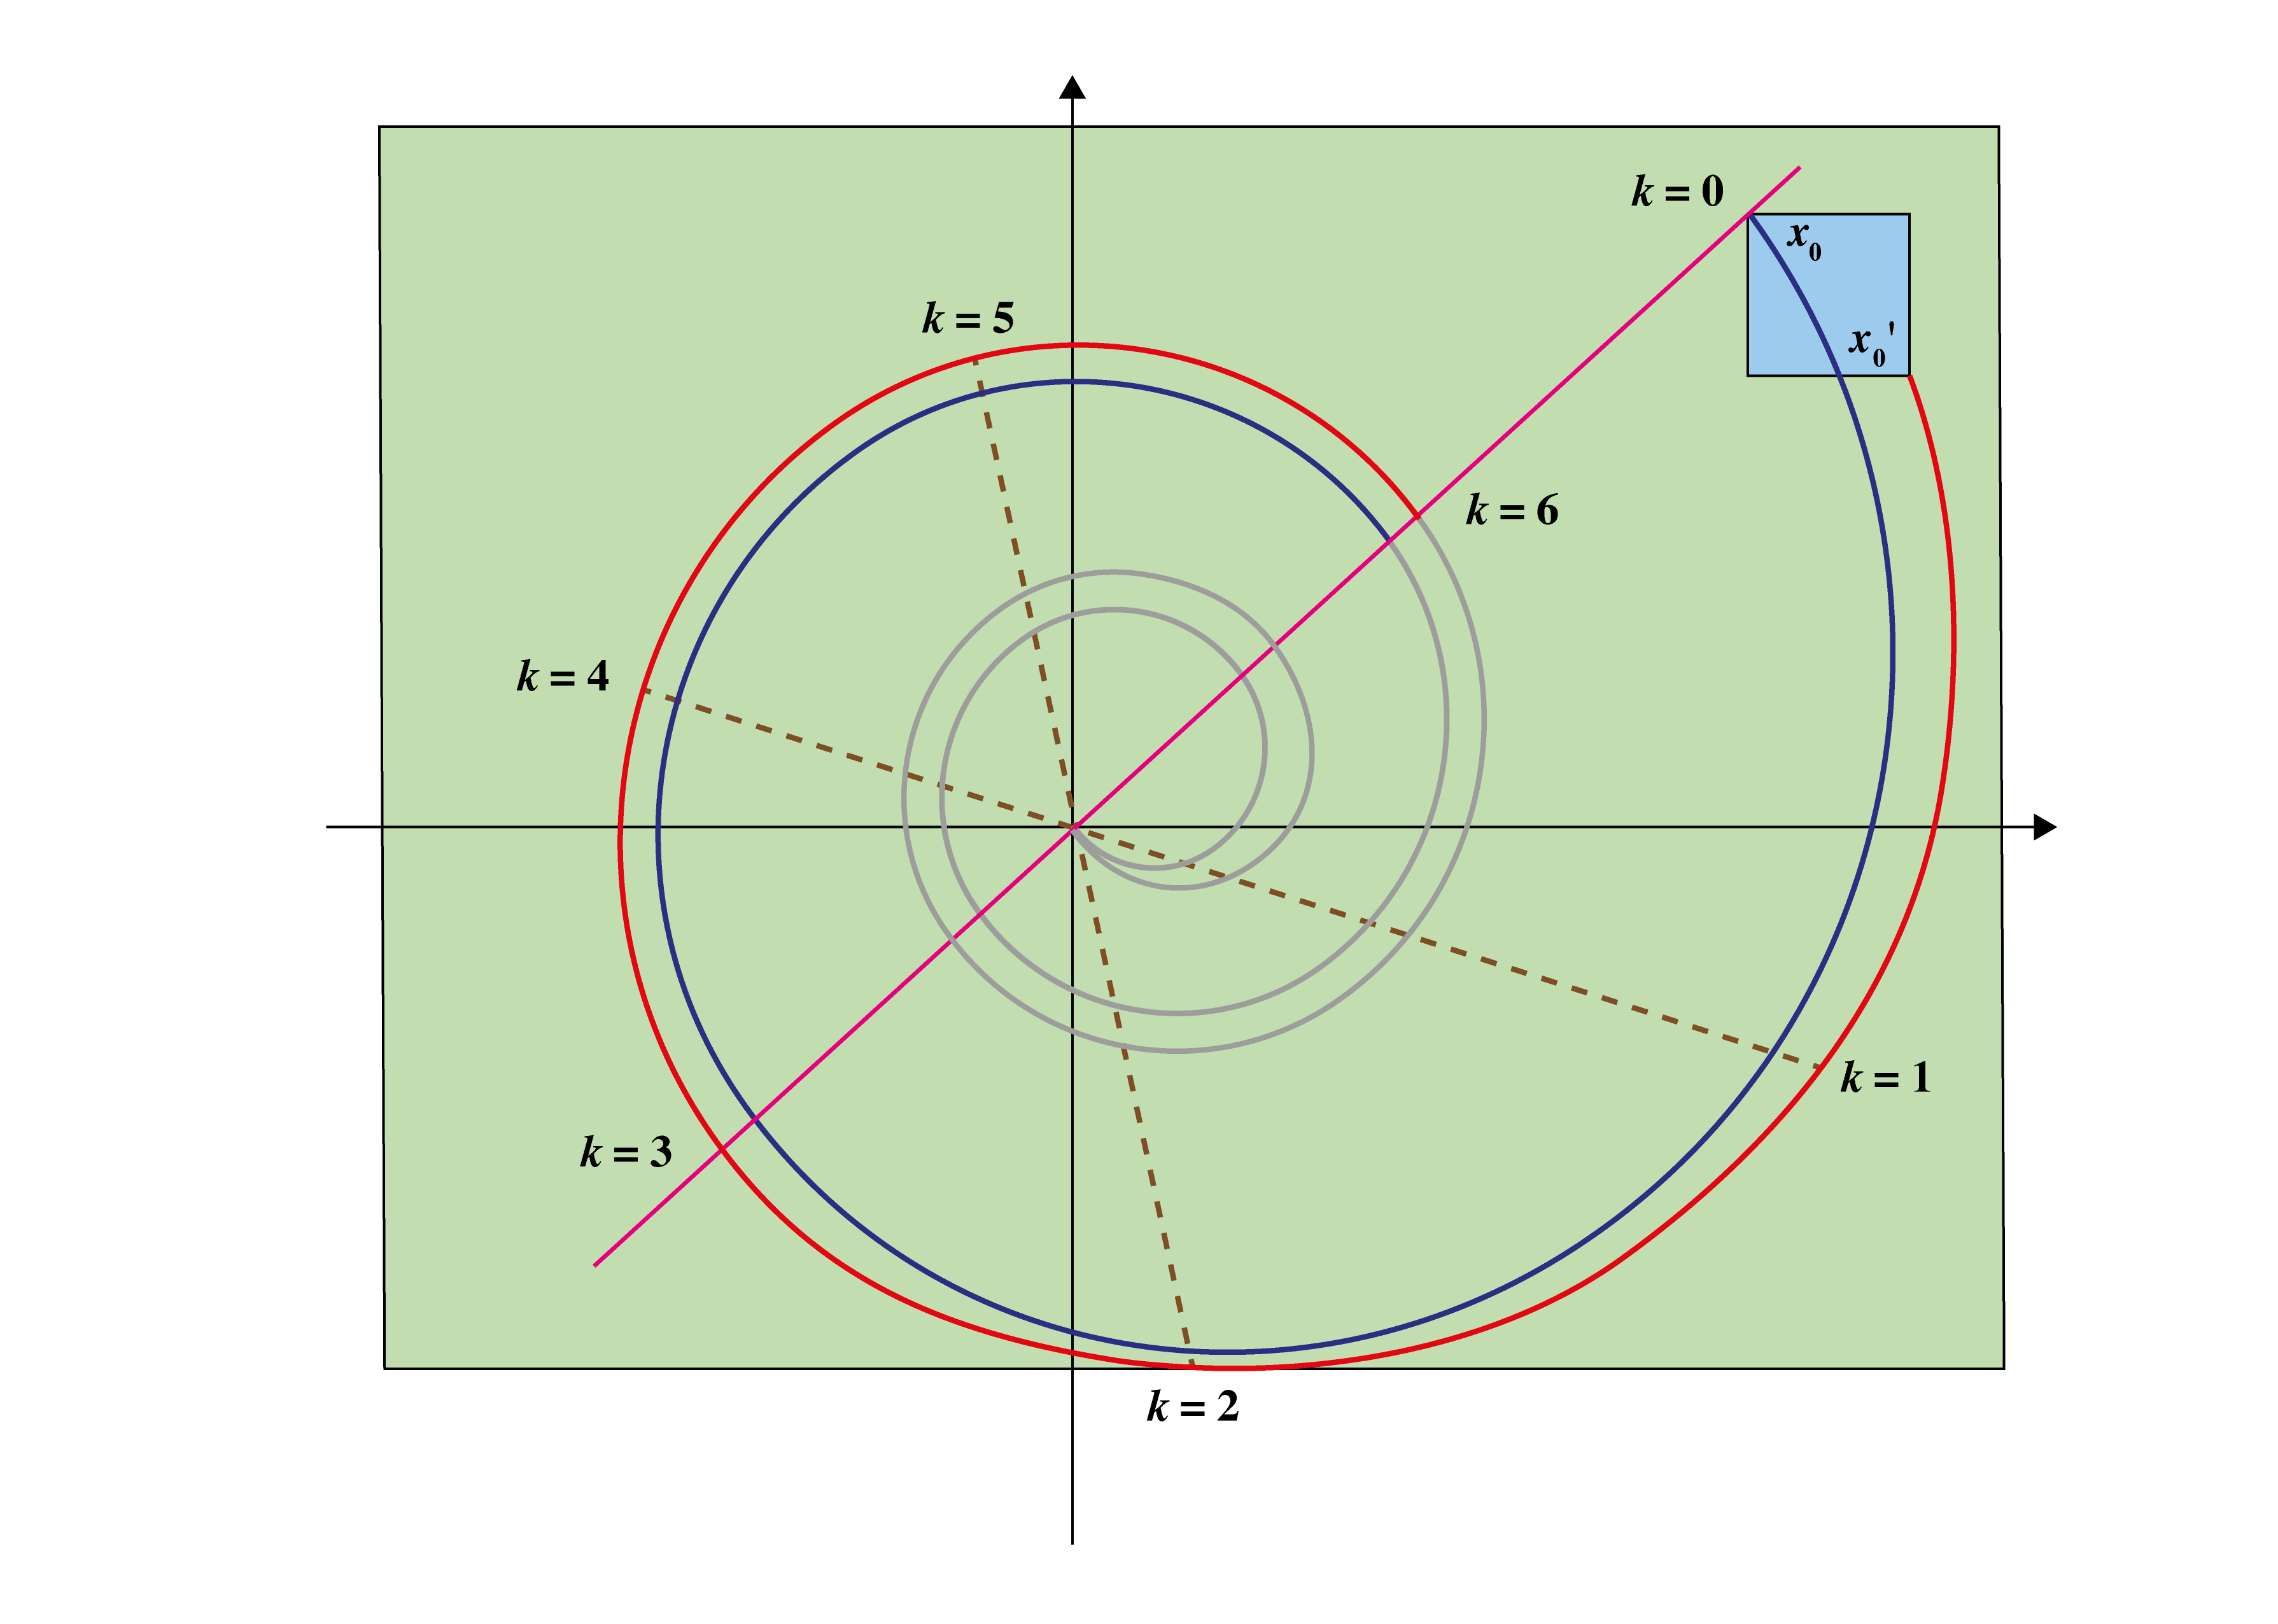
\includegraphics[width=.55\textwidth]{figures/spirals/Spirals-06-prime.png}
 \end{overprint}
%}
\end{tabular}

\end{frame}





\begin{frame}{Experimental results}
  
\begin{table}
\centering
\scriptsize
\begin{tabular}{| r | l | c | c | r |}
%
\hline
\# & \multicolumn{1}{|c|}{Benchmark} & \multicolumn{1}{|c|}{Order} & \multicolumn{2}{|c|}{Completeness threshold}                 \\
   &                                  & & \multicolumn{1}{|c|}{$\langle I_p,F_p \rangle$} & \multicolumn{1}{|c|}{Time} \\\hline
1  & {\bf Cruise Control}  & 1 & \cellcolor{green!40}8,16   & \cellcolor{green!40}7.44\,s \\
2  & {\bf DC Motor}          & 2 & \cellcolor{green!40}8,16   & \cellcolor{green!40}7.76\,s\\
3  & {\bf Helicopter}        & 3 & \cellcolor{green!40}8,16 &  \cellcolor{green!40}12.13\,s \\
4  & {\bf Inverted Pendulum} & 4 & \cellcolor{green!40}8,16   & \cellcolor{green!40}8.82\,s \\
5  & {\bf Magnetic Pointer}  & 2 & \cellcolor{green!40}8,16 &  \cellcolor{green!40}10.31\,s \\
6  & {\bf Magnetic Suspension} & 2 & \cellcolor{green!40}12,20  & \cellcolor{green!40}21.55\,s \\
7  & {\bf Pendulum}          & 2 & \cellcolor{green!40}8,16   & \cellcolor{green!40}9.08\,s \\
8  & {\bf Suspension}        & 2 & \cellcolor{green!40}8,16  & \cellcolor{green!40}17.18\,s \\
9  & {\bf Tape Driver}       & 3 & \cellcolor{green!40}8,16   & \cellcolor{green!40}8.05\,s \\
10 & {\bf Satellite}          & 2 & \cellcolor{green!40}8,16   & \cellcolor{green!40}8.76\,s \\\hline
%
\end{tabular}
\end{table}

\uncover<2->{
\small
\begin{tabular}{p{\dimexpr 0.5\linewidth-2\tabcolsep} 
    p{\dimexpr 0.5\linewidth-2\tabcolsep}}

  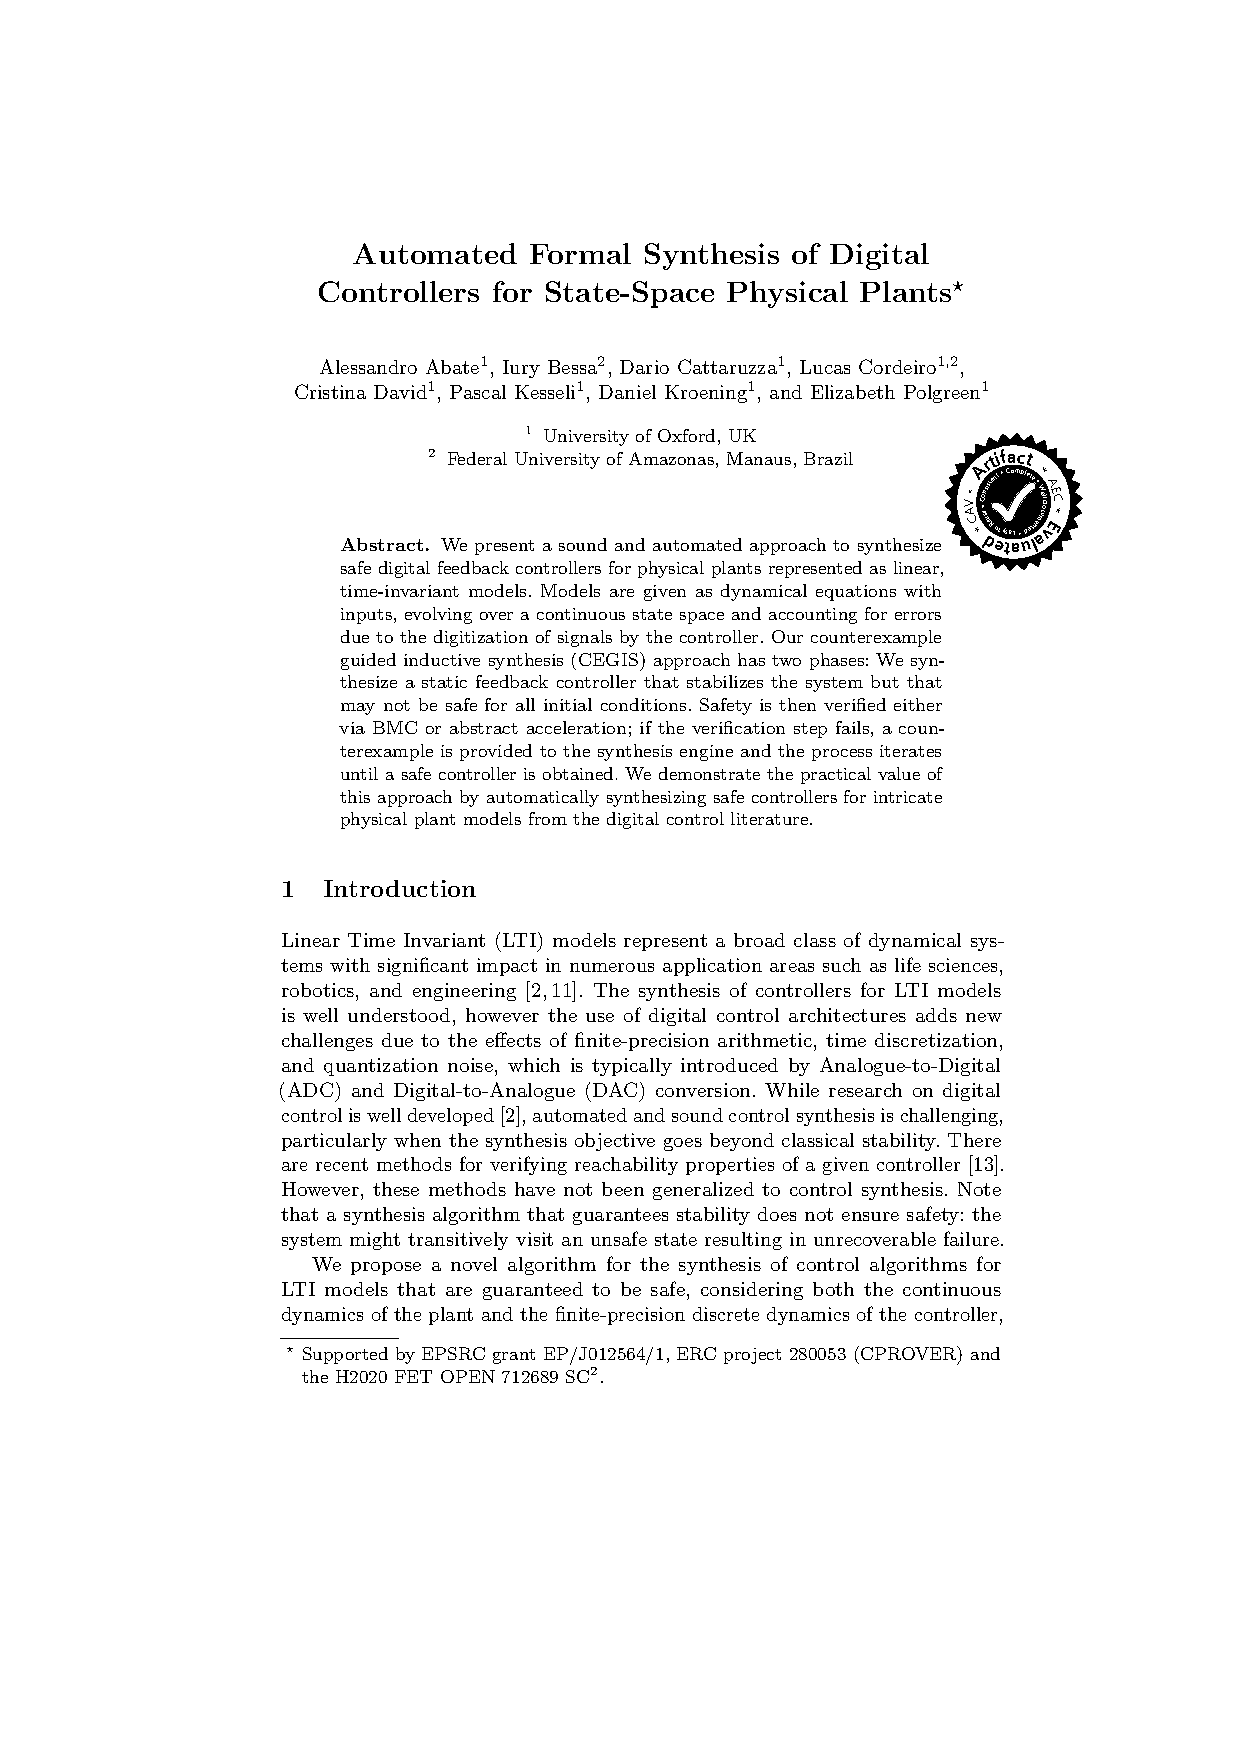
\includegraphics[width=.18\textwidth]{figures/cav2017frontpage.pdf} &
\begin{tabular}{l}  
\hspace{-4cm}
Check abstract acceleration based approach in the paper!\\\\\\\\\\\\
\end{tabular}
\end{tabular}
}
\end{frame}


\begin{frame}{Conclusions}

We built an {\bf automated synthesizer for digital state-feedback
controllers} that ensures both {\bf stability} and {\bf safety}

\vspace{.5cm}

We considered the errors caused by the implementation of the digital control
algorithm and the modeling of plant dynamics

\only<2->{
\vspace{.5cm}
\begin{tabular}{cc}
  \scriptsize
  \begin{tabular}{l}
  {\bf DSSynth Matlab toolbox:}\\
  http://dsverifier.org/dsverifier/dssynth-toolbox/
  \\\\\\\\\\\\
  \end{tabular}
  &
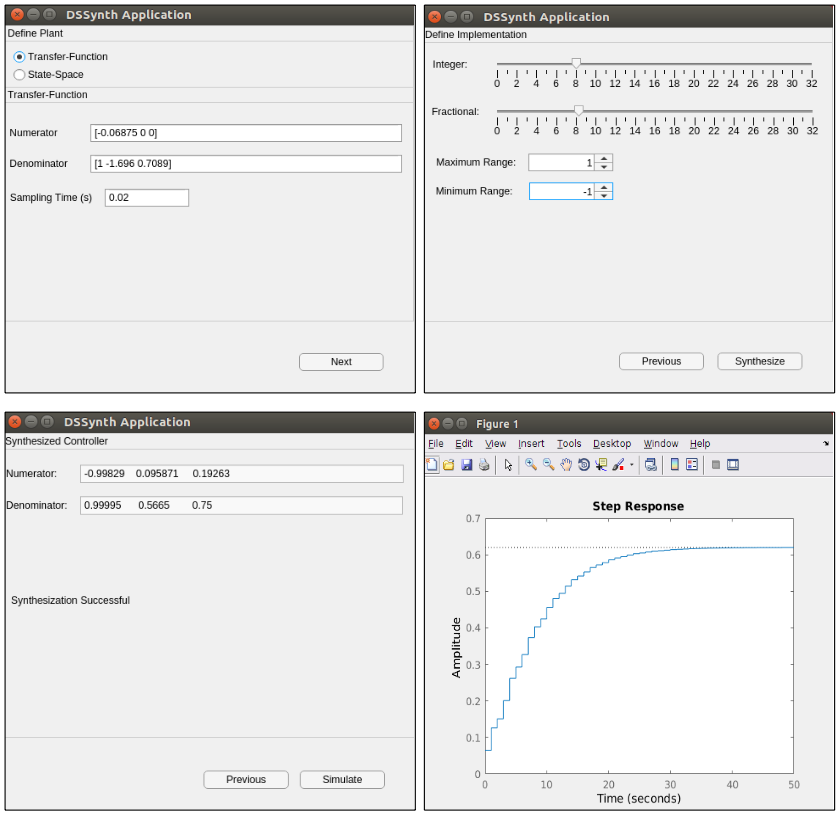
\includegraphics[width=.35\textwidth]{figures/screens_dssynth.png}
\end{tabular}
}
\end{frame}  


\begin{frame}{Abstraction-based controller synthesis}
\vspace{-1cm}
\resizebox{.9\textwidth}{!}
{
\centering
{\scriptsize
  \begin{tikzpicture}[scale=0.3,->,>=stealth',shorten >=.2pt,auto, semithick, ampersand replacement=\&,]
  \matrix[nodes={draw, fill=none, shape=rectangle, minimum height=.2cm, minimum width=.2cm, align=center},row sep=1.5cm, column sep=2cm] {
   \coordinate (aux1);
   \& \coordinate (aux2);
   \& ;\\
   %\& \node[fill=gray!20,align=center] (abstract) {\sc 4. abstract};
   %\& \coordinate (aux); \\ 
   \& \node[fill=gray!20,align=center] (synth) {\sc 2. synthesize};
    \only<2,7>{\node[fill=red!20,align=center] (synth) {\sc 2. synthesize};}   
   \& \node[fill=gray!20,align=center, minimum width=3.5cm] (verify) {\sc 3. verify };
   \only<3,6,8,10>{\node[fill=red!20,align=center, minimum width=3.5cm] (verify) {\sc 3. verify ($\phi$)};}
   \& \node[ellipse, fill=gray!20] (done) {{\sc Done}};
   \only<10>{\node[ellipse, fill=red!20] (done) {{\sc Done}};}\\   
   \& \node[draw,rectangle,align=center] (KSAT) {Program \\ Search};
   \& complexnode/.pic={
     \coordinate (AA);
     \node[draw,rectangle,align=center] (AAV) at ([xshift=-1.5cm]AA.center) {Abstract\\Acceleration};
     \only<3,5,8>{\node[draw,fill=red!20,rectangle,align=center] (AAV) at ([xshift=-1.5cm]AA.center) {Abstract\\Acceleration};}
     \node[draw,rectangle,align=center] (AAC) at ([xshift=1.5cm]AA.center) {Abstraction \\ Verifier};
     \only<4,6,9>{\node[draw,fill=red!20,rectangle,align=center] (AAC) at ([xshift=1.5cm]AA.center) {Abstraction \\ Verifier};}
   }
   \& \\   
  };
  %\path (abstract.south) edge node{$\textcolor{blue}{\begin{array}{c}\phi_{init}^K\\P_a(z)\\k=0\end{array}}$} (synth.north);
    \path ([yshift=1em]synth.east) edge node {$C$} ([yshift=1em]verify.west);
    \path ([yshift=-1em]verify.west) edge node{$(k, x_0)$} ([yshift=-1em]synth.east);
    %\path (aux) edge (abstract.east);
    \path(verify.east) edge (done.west);

  \path ([xshift=+.6cm]KSAT.north) edge[left] node[xshift=-.3cm] {} ([xshift=0.6cm]synth.south);
   \path ([xshift=-.6cm]synth.south) edge node[align=center,xshift=.3cm] {} ([xshift=-.6cm]KSAT.north);
    \path ([yshift=.5cm]AAV.east) edge node{\sl $\hat{X}$} ([yshift=.5cm]AAC.west);
    \path ([yshift=-.5cm]AAC.west) edge node{} ([yshift=-.5cm]AAV.east);
    \path (AAC.north) edge node{} ([xshift=4.9cm]verify.south);
    \path ([xshift=-5cm]verify.south) edge node{$C$} (AAV.north);

\end{tikzpicture}
}}


 \scriptsize
 %&
 \begin{tabular}{p{\dimexpr 0.5\linewidth-2\tabcolsep} 
     p{\dimexpr 0.5\linewidth-2\tabcolsep}}

   \only<2>{
     \begin{tabular}{l}
       {\bf Find controller for given $\{x_0\}$ and $\{k\}$}\\
       {\bf such that the system is stable and safe}
     \\\\\\\\\\\\\\\\\\\\\\\\\\\\\\
  \end{tabular}
   }
   \only<3>{
     \begin{tabular}{l}
     {\bf Use abstract acceleration to compute an} \\
     {\bf overapproximation the set of all reachable}\\
     {\bf states at all times}\\
     \\\\\\\\\\\\\\\\\\\\\\\\\\
  \end{tabular}
   }
   \only<4>{
     \begin{tabular}{l}
       {\bf Find an initial state and a number of}\\
       {\bf iterations for for which the system is unsafe} \\
     \\\\\\\\\\\\\\\\\\\\\\\\\\\\ 
  \end{tabular}
   }
   \only<5>{
     \begin{tabular}{l}
     {\bf Refine abstraction} \\
     \\\\\\\\\\\\\\\\\\\\\\\\\\\\\\     
  \end{tabular}
   }
   \only<6>{
     \begin{tabular}{l}
     {\bf Real counterexample $(x_0', k')$ found} \\
     \\\\\\\\\\\\\\\\\\\\\\\\\\\\\\   
  \end{tabular}
   }
   \only<7>{
     \begin{tabular}{l}
       {\bf Find controller for given $\{x_0, x_0'\}$ and $\{k, k'\}$}\\
       {\bf such that the system is stable and safe}
     \\\\\\\\\\\\\\\\\\\\\\\\\\\\\\
  \end{tabular}
   }
   \only<8>{
     \begin{tabular}{l}
     {\bf Use abstract acceleration to compute an} \\
     {\bf overapproximation the set of all reachable}\\
     {\bf states at all times}\\
     \\\\\\\\\\\\\\\\\\\\\\\\\\
  \end{tabular}
   }
   \only<9>{
     \begin{tabular}{l}
       {\bf Find an initial state and a number of iterations}\\
       {\bf for which the system is unsafe} \\
     \\\\\\\\\\\\\\\\\\\\\\\\\\\\
  \end{tabular}
   }
   \only<10>{
     \begin{tabular}{l}
     {\bf Controller found} \\
     \\\\\\\\\\\\\\\\\\\\\\\\\\\\\\        
  \end{tabular}
   }

   &
 \only<2>{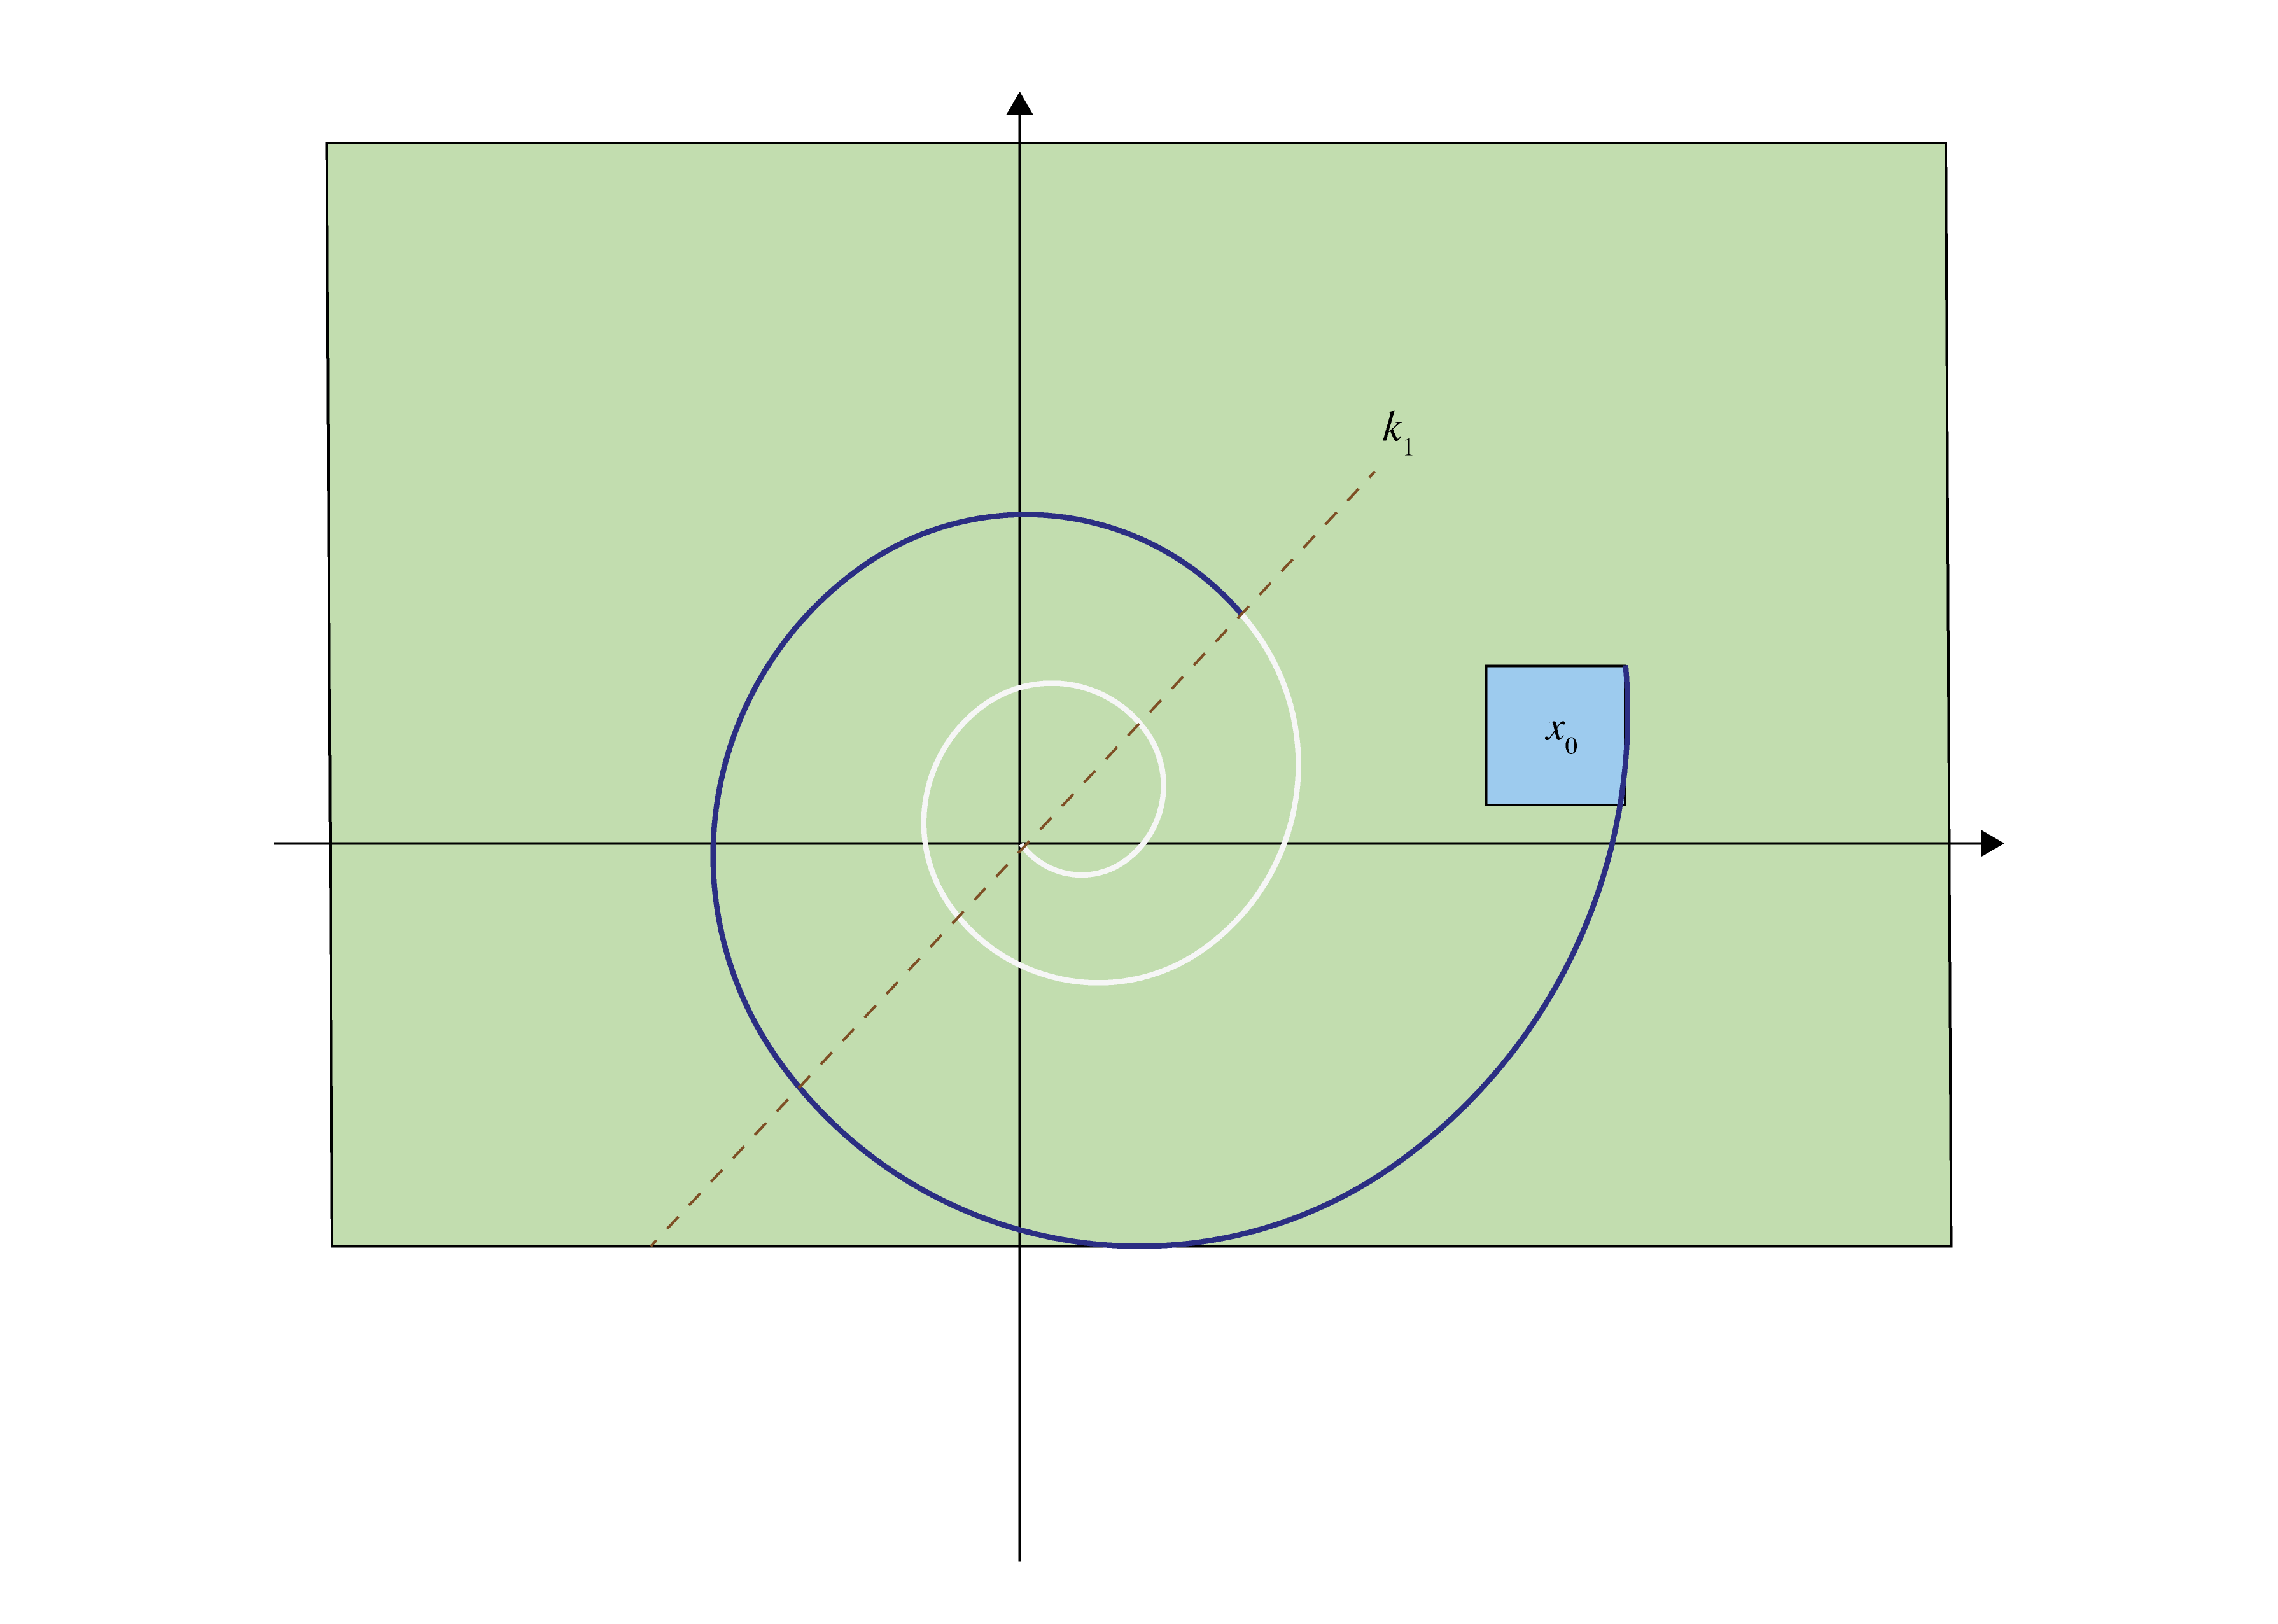
\includegraphics[width=.6\textwidth]{figures/spirals/Spirals-11.png}}
 \only<3>{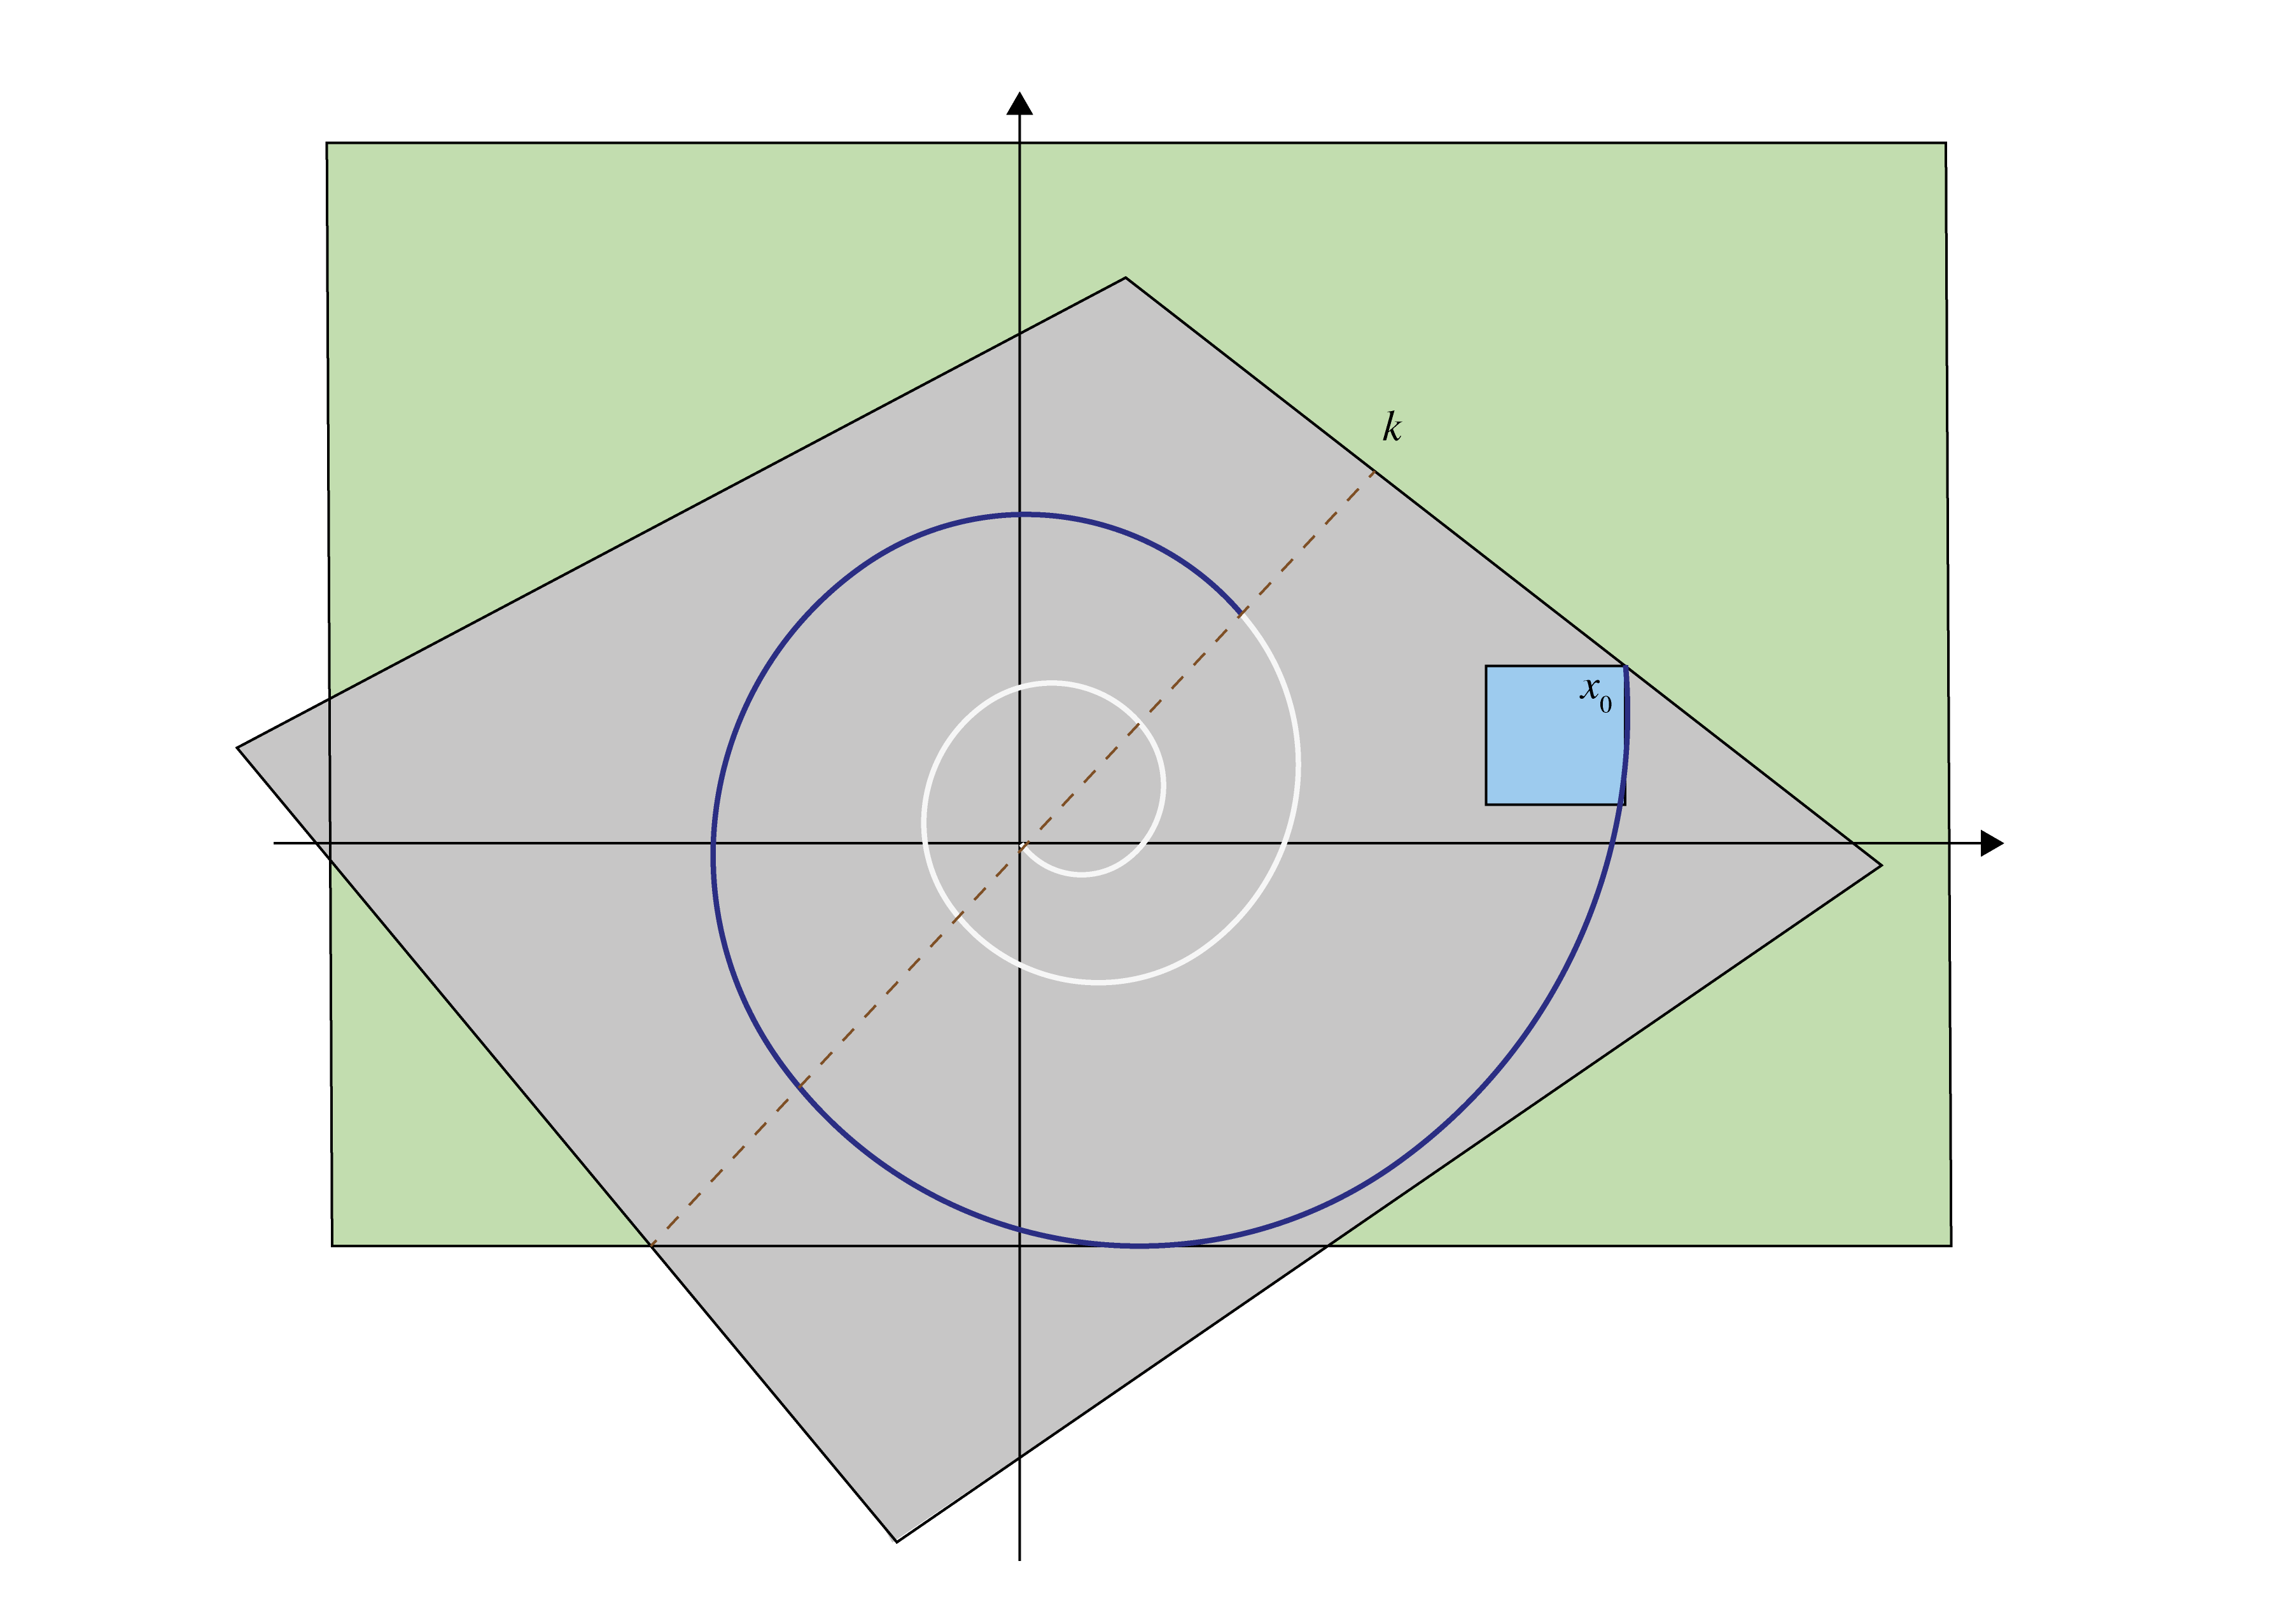
\includegraphics[width=.6\textwidth]{figures/spirals/Spirals-07.png}}
 \only<4>{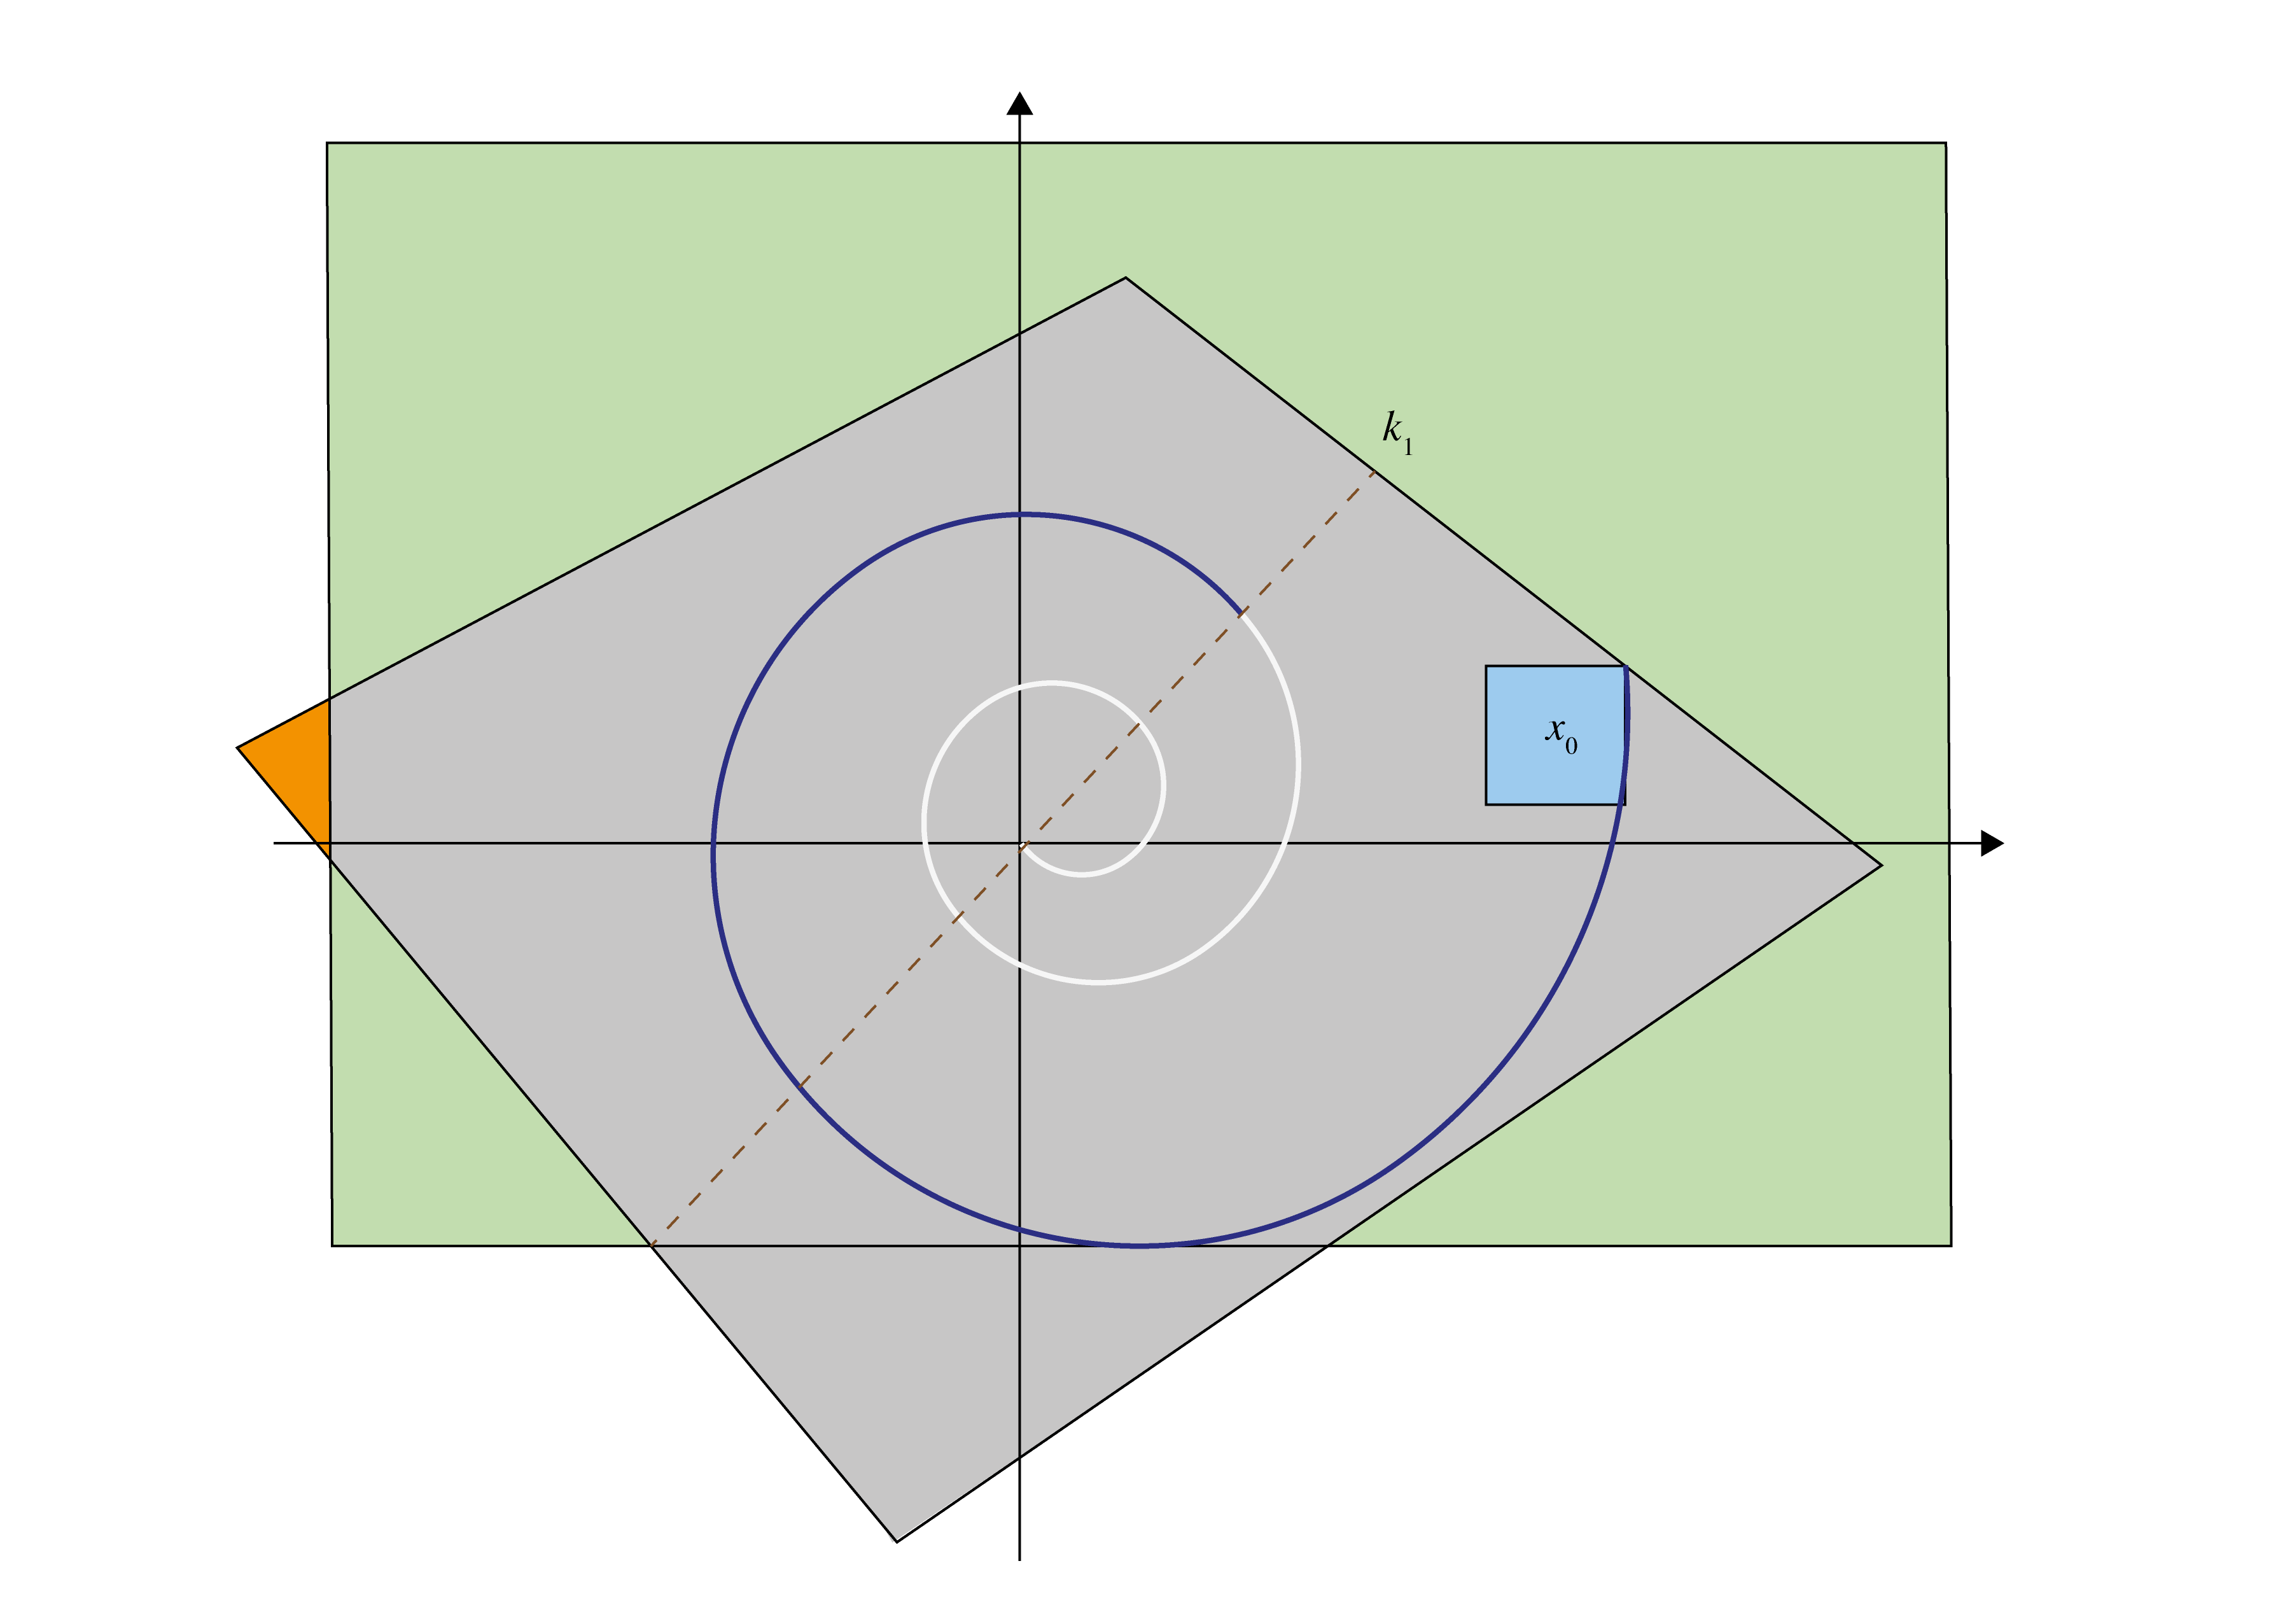
\includegraphics[width=.6\textwidth]{figures/spirals/Spirals-08.png}}
 \only<5>{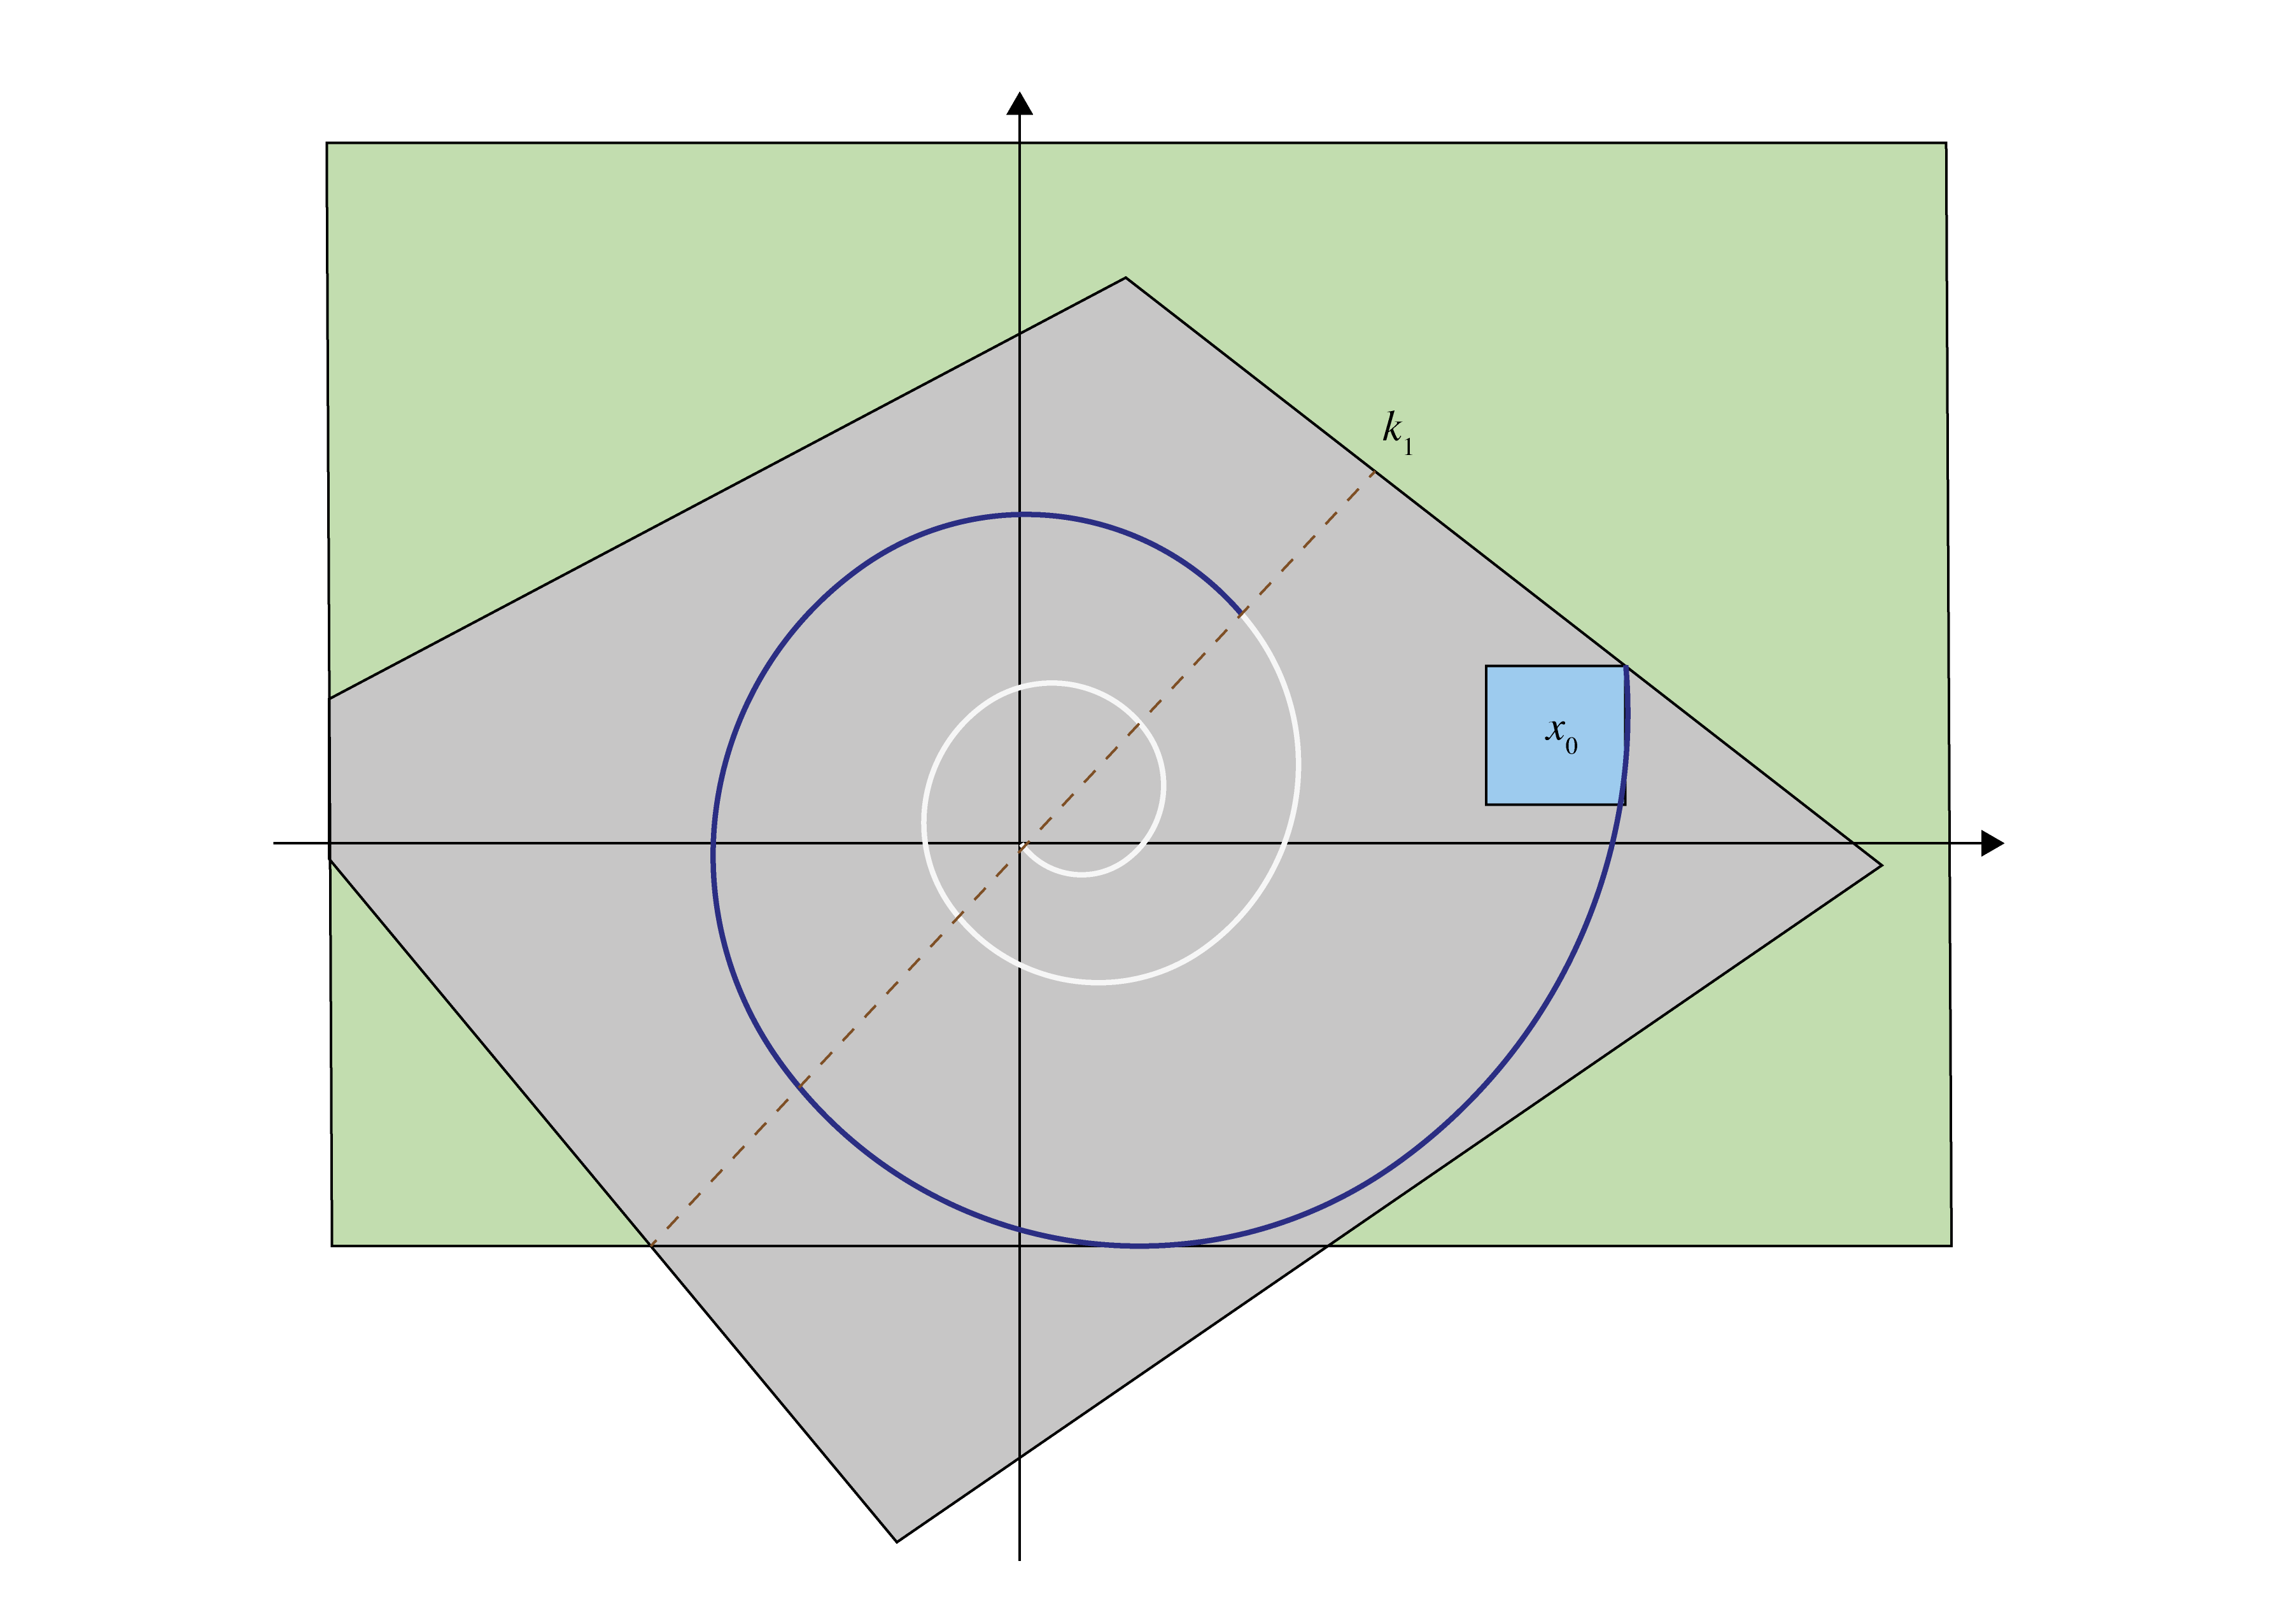
\includegraphics[width=.6\textwidth]{figures/spirals/Spirals-09.png}}    
 \only<6>{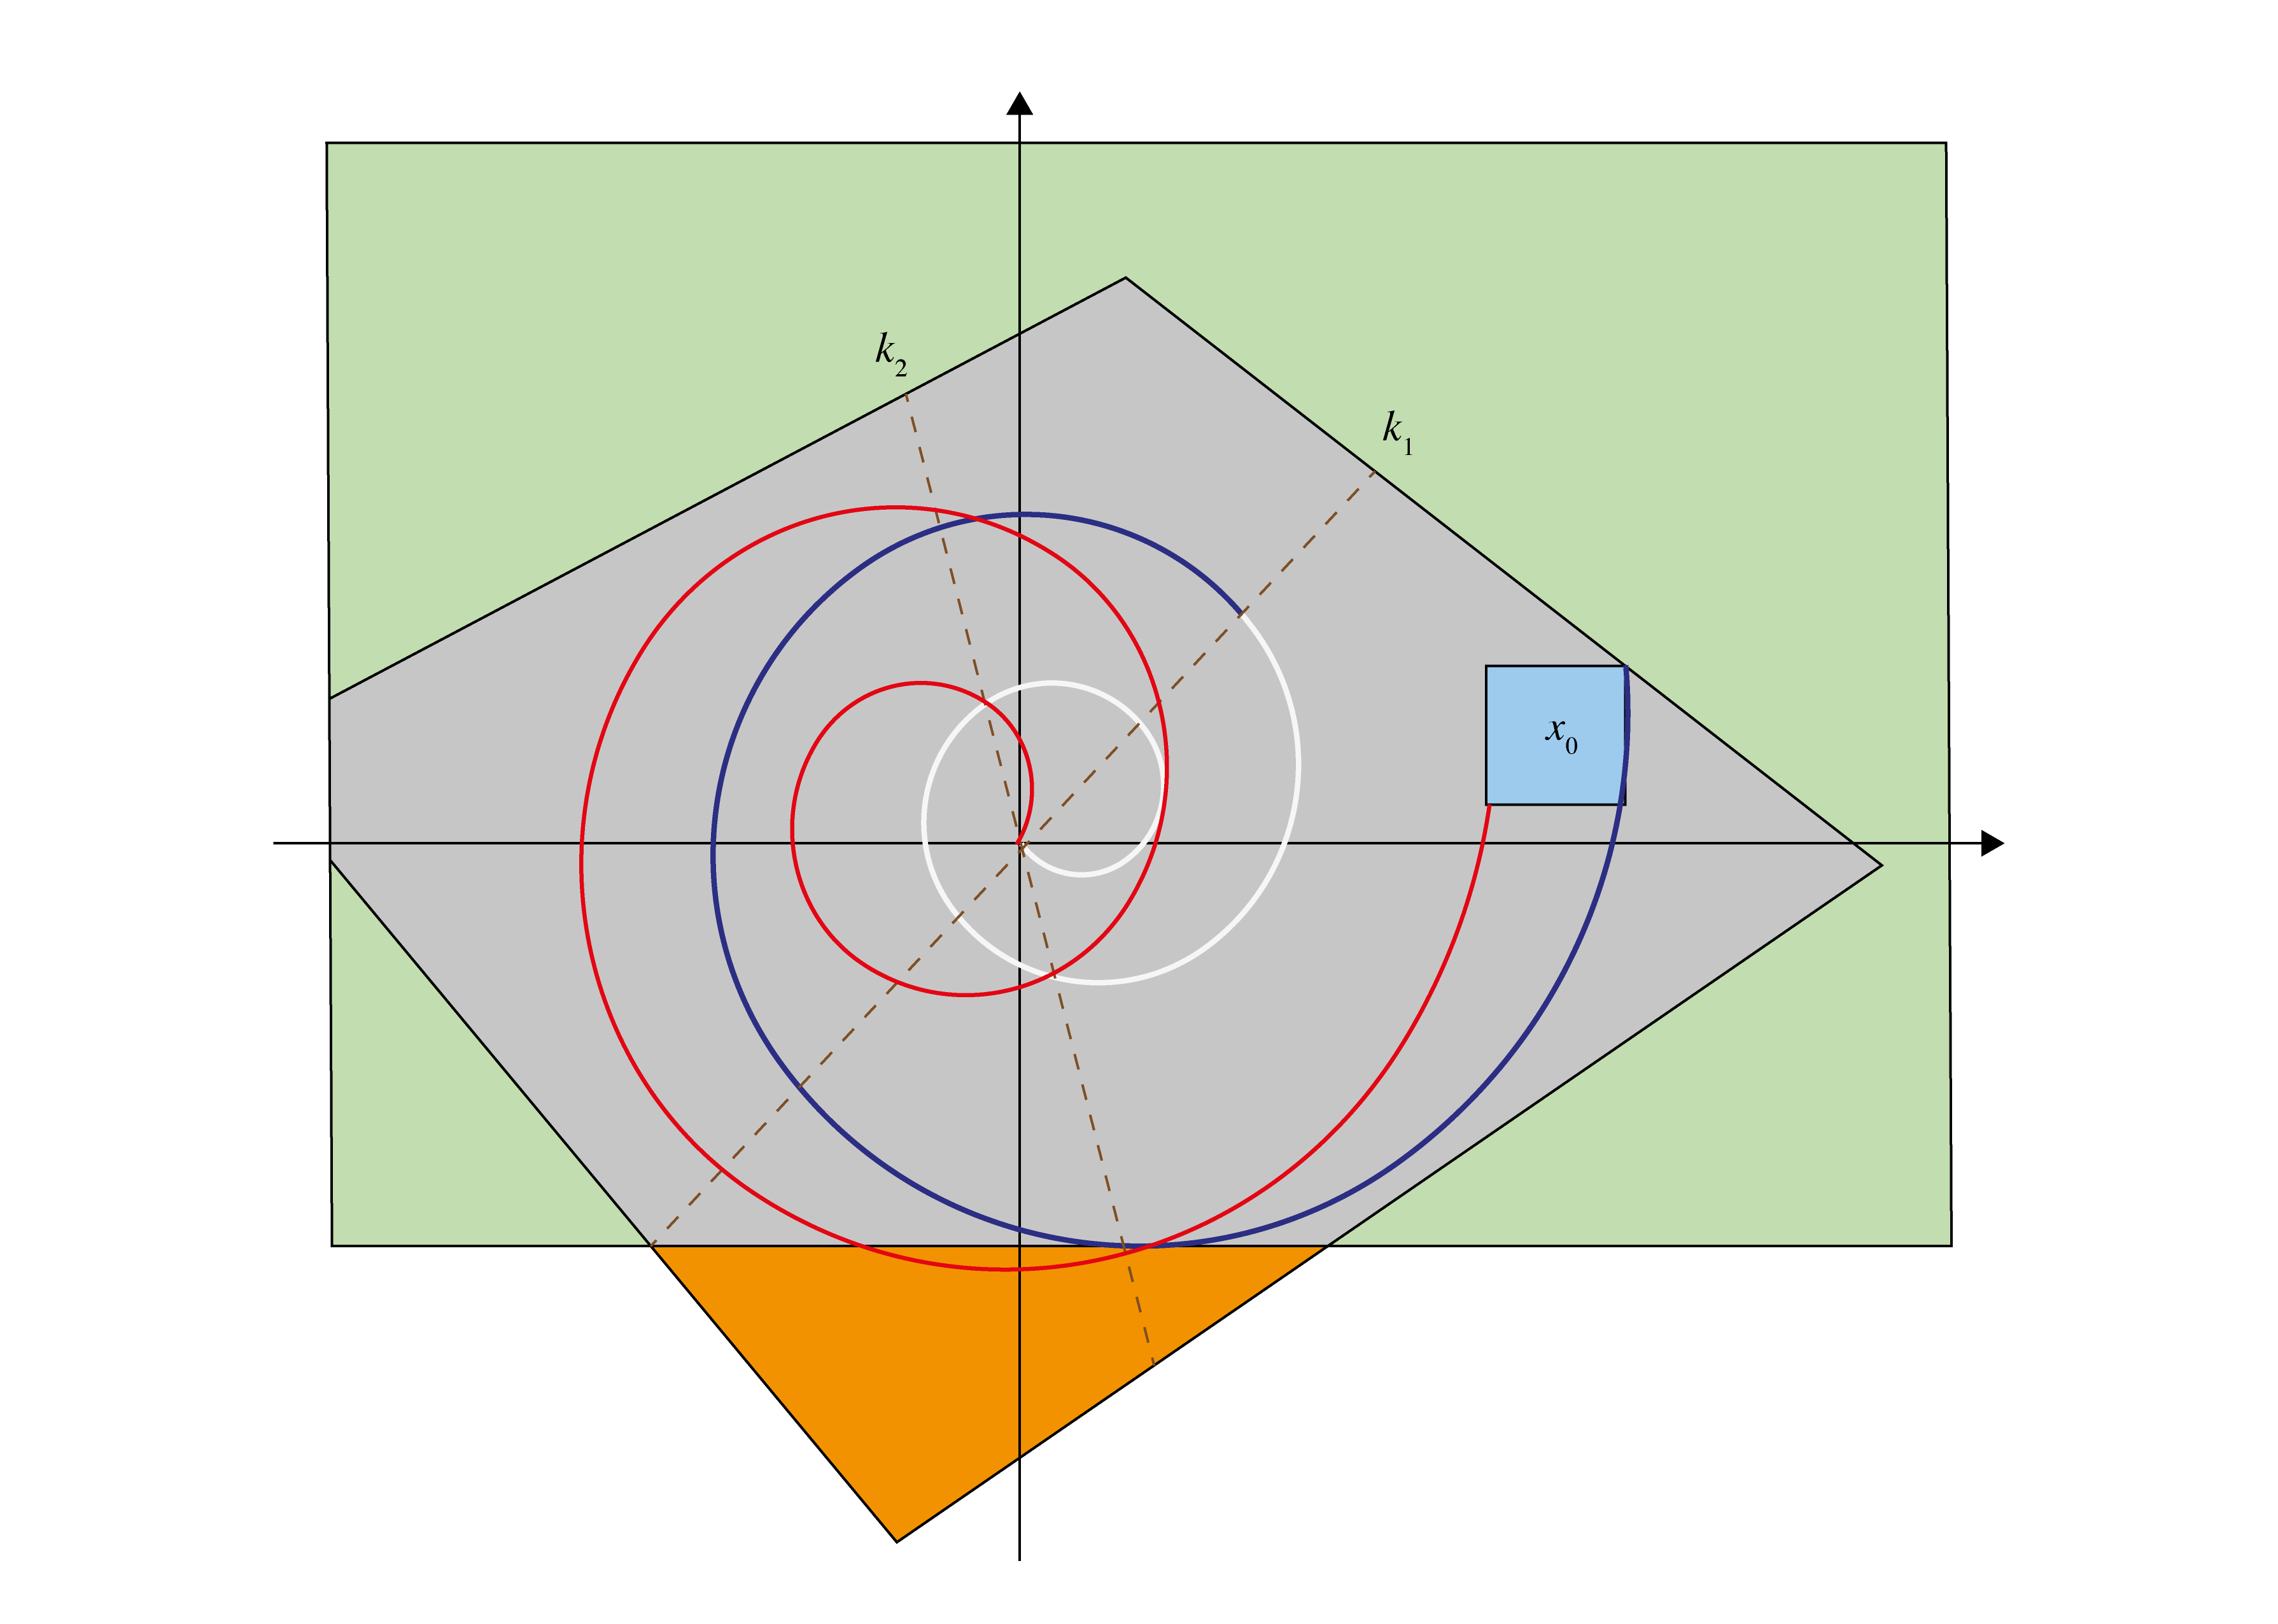
\includegraphics[width=.6\textwidth]{figures/spirals/Spirals-10.png}}
 \only<7>{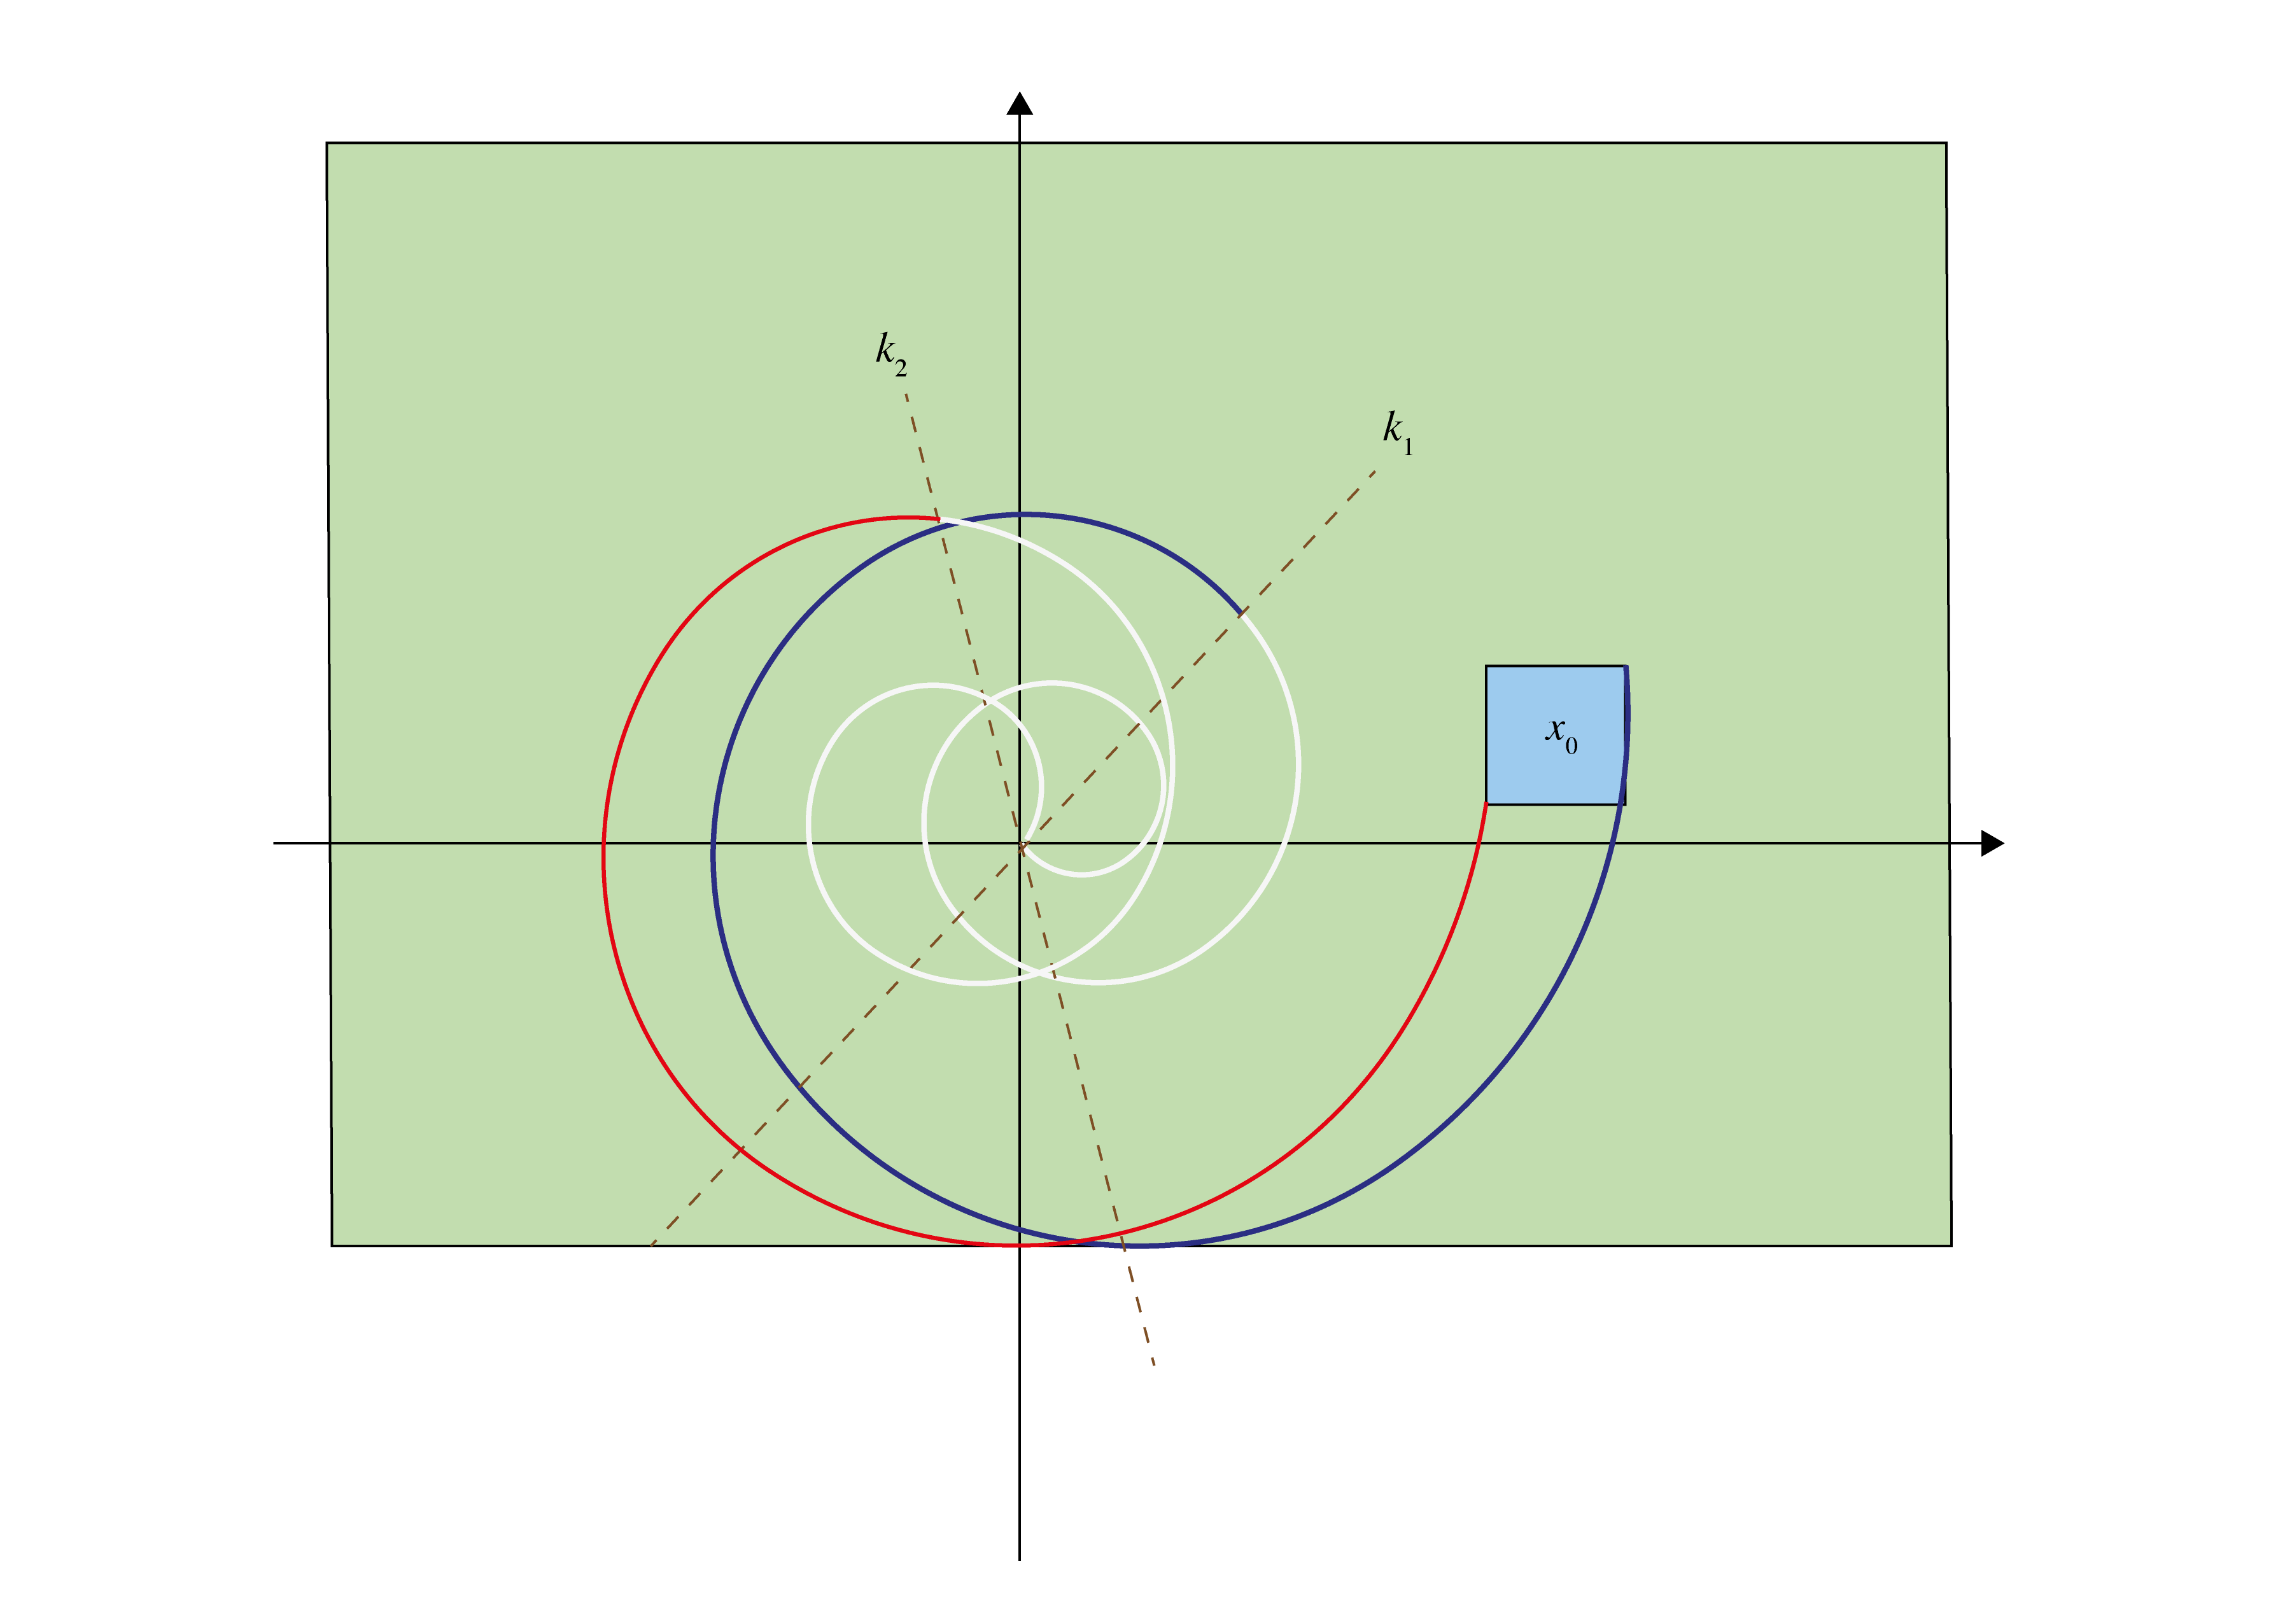
\includegraphics[width=.6\textwidth]{figures/spirals/Spirals-12.png}}
 \only<8->{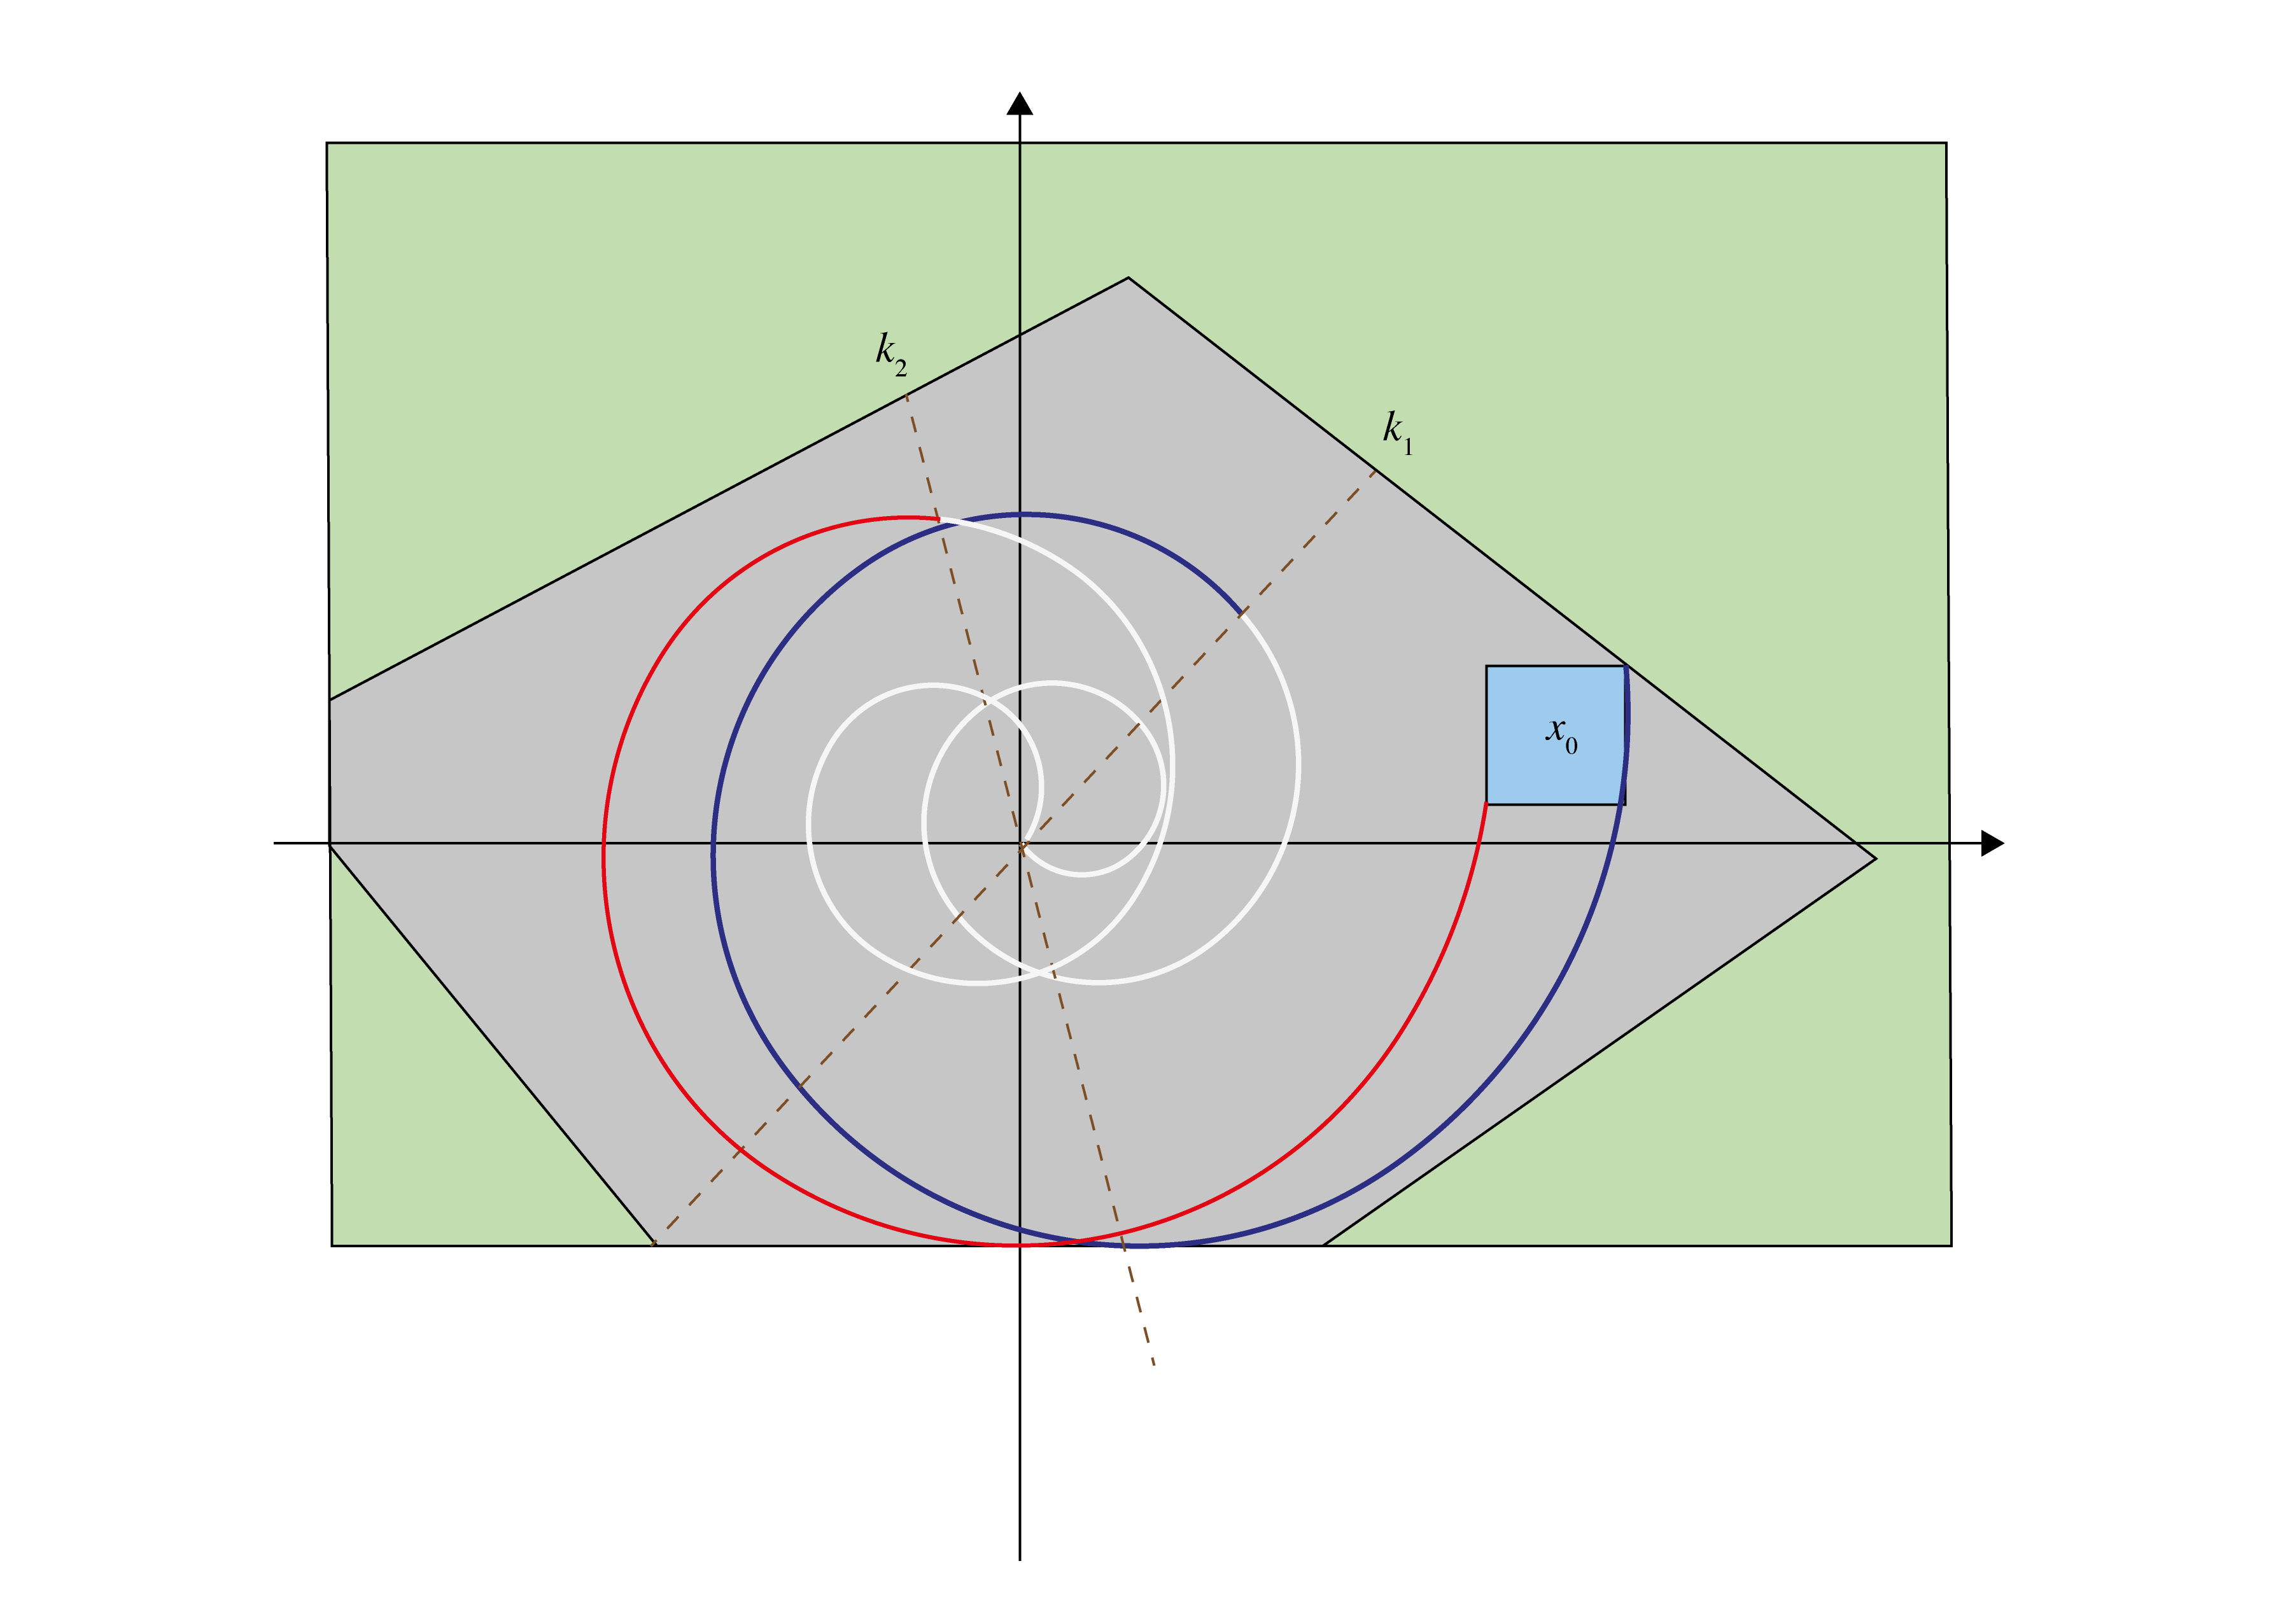
\includegraphics[width=.6\textwidth]{figures/spirals/Spirals-13.png}} 

\end{tabular} 

%[figure]: one spiral with abstract acceleration but no red area, just gray.
 %[figure]: refine abstraction: spiral with two red areas, one spurious and one with a
 % real c-ex.
 %[figure]: two spirals within green area; add grey polygon (inside green area). 
\end{frame}  


\end{document}
